\documentclass[11pt]{beamer}
\usepackage{graphicx}
\usepackage[export]{adjustbox}  % max width/height in includegraphics
\usepackage[framemethod=TikZ]{mdframed}
\usepackage[document]{ragged2e}
\usepackage{soul}
\usepackage{xcolor}
\usepackage{ifthen}
\usepackage{fontspec}
\usepackage{textcomp}
%\usepackage[T5,T1]{fontenc}
\usepackage{caption}

\usetheme[hideothersubsections]{Goettingen}
\usecolortheme{seahorse}
%%% \usetheme{Montpellier}
%%% \usecolortheme{dolphin}
\setbeamercovered{invisible}
\setbeamertemplate{navigation symbols}{\insertslidenavigationsymbol}
\setbeamertemplate{page number in head/foot}{}
\setbeamertemplate{blocks}[rounded][shadow=false]
% \setbeamerfont{section in sidebar}{size=\fontsize{4}{3}\selectfont}
% \setbeamerfont{subsection in sidebar}{size=\fontsize{4}{3}\selectfont}
% \setbeamerfont{subsubsection in sidebar}{size=\fontsize{4}{2}\selectfont}


\usepackage{microtype}
% \DisableLigatures[f]{encoding = *, family = *}

% \usefonttheme{professionalfonts} % using non standard fonts for beamer
\usepackage{tgheros}
\usefonttheme{serif}
\usepackage{XCharter}

\AtBeginSection[]{
  \begin{frame}
    \vfill
    \centering
    \begin{beamercolorbox}[sep=8pt,center,shadow=true,rounded=true]{title}
    \usebeamerfont{title}\insertsectionhead\par%
    \ifthenelse{\equal{\thisSectionName}{Bonus}}{}{
        \usebeamerfont{subtitle}\thisSectionName\par%
    }
    \end{beamercolorbox}
    \begin{center}
    \ifthenelse{\equal{\thisSectionName}{Colleges and Universities}}{
        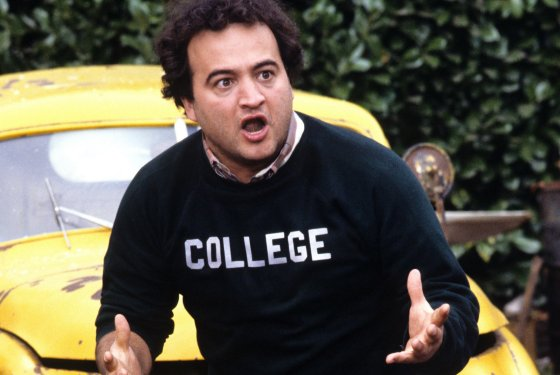
\includegraphics[max height = 0.3\textheight]{Images/belushicollege.jpg}
    }{}

    Please mute yourselves!
    \end{center}

    \ifthenelse{\equal{\thisSectionName}{Bonus}}
    {
        Get ready for some \emph{devilishly} hard questions!

        \vspace*{1em}
        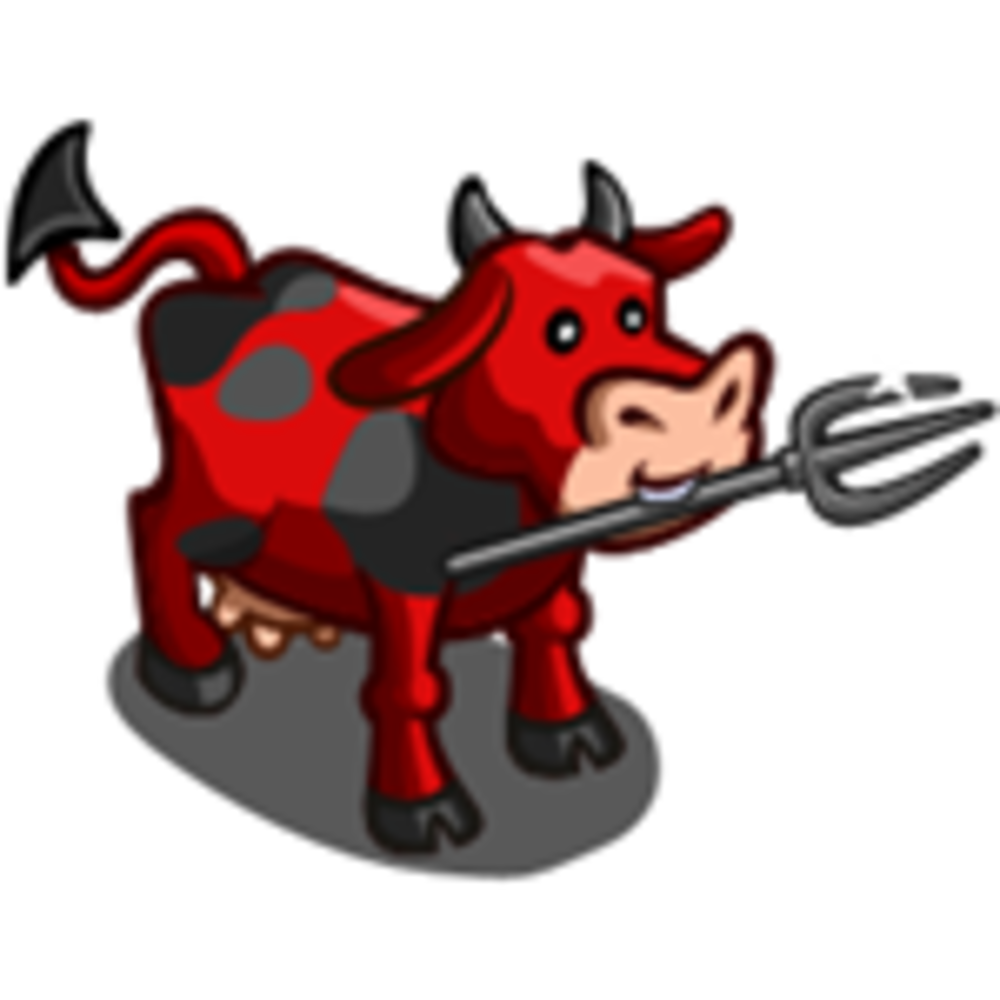
\includegraphics[max width=0.5\textwidth,
           max height=0.4\textheight]{Images/devil.png}
    }{}

    \vfill
  \end{frame}
}

\AtBeginSubsection[]{
  \begin{frame}
    \vfill
    \centering
    \begin{beamercolorbox}[sep=8pt,center,shadow=true,rounded=true]{title}
    \usebeamerfont{title}\insertsectionhead\par%
    \usebeamerfont{subtitle}\insertsubsectionhead\par%
    \end{beamercolorbox}
    \ifthenelse{\equal{\subsecname}{Answers}} {
        \begin{center}
        Unmute yourselves!
        \end{center}
    }
    \vfill
  \end{frame}
}
\begin{document}

\title{Welcome to Quarantine Trivia XI!}
\date{}

\begin{frame}
\titlepage{}
\begin{center}

\includegraphics[max width=0.9\textwidth,
    max height=0.4\textheight]{Images/triviatitleframelogo.png}
\end{center}
\end{frame}
\begin{frame}
Each week it seems as though there is a discussion about a particular question. Last
week, the discussion was about the principal shopping street in Rome. The answer we gave
was Via del Corso, but many players suggested other streets. So we checked with an
expert, our cousin Luciana, a native of Rome.

\begin{center}
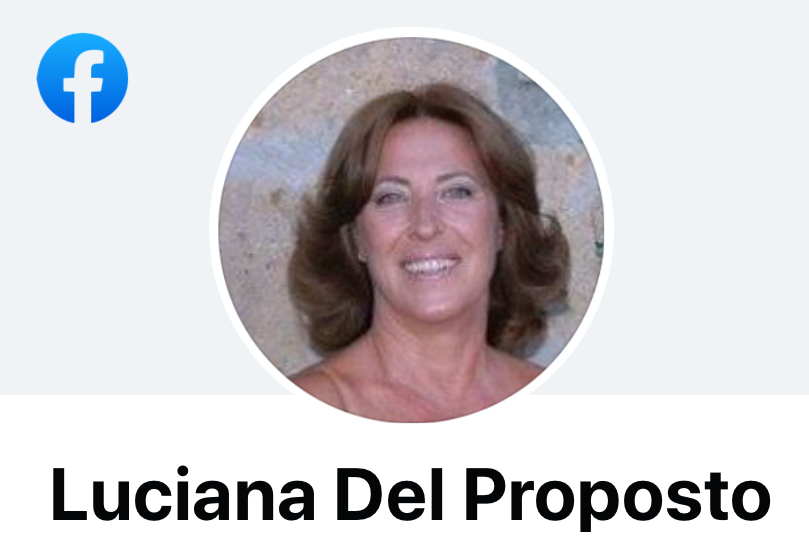
\includegraphics[max width=.9\textwidth,max height=.4\textheight
]{Images/luciana.jpg}
\end{center}
\end{frame}

\begingroup{}
\begin{frame}{}
\hfill{}\begin{minipage}{0.9\textwidth}
\begin{mdframed}[
    roundcorner=7pt,
    backgroundcolor=blue!80!white,
    linecolor=blue!80!white,
    fontcolor=white,
    ignorelastdescenders]
\begin{flushleft}
{\small{}\fontfamily{qhv}\selectfont{}
Luciana,

Una richiesta: Puoi risolvere una discussione fra qualche amico (incluso me) quanto a
Roma? La domanda: Come romana, come nativa di Roma, secondo te, quale via e
\ul{\textbf{la via principale a Roma per lo shopping}}?
Non ti dico la mia opinione perché non voglio influenzare la tua riposta.

Grazie mille. Ciao a Guiseppe.

Terry
}
\end{flushleft}
\end{mdframed}
\end{minipage}

\begin{minipage}{0.9\textwidth}
\begin{mdframed}[
    roundcorner=7pt,
    backgroundcolor=black!5,
    linecolor=black!5,
    fontcolor=black,
    ignorelastdescenders]
\begin{flushleft}
{\small{}\fontfamily{qhv}\selectfont{}
La zona più amata da tutti noi è da piazza di Spagna a piazza del Popolo. Tutte quelle
strade sono le più frequentate per lo shopping.
\ul{\textbf{Via del Corso}},
via della Vite, viadelle Carrozze, via del Babuino, via dei Condotti, via
Frattina, via del Gambero etc etc. Poi ci sono romani, come me, che non amano le strade
affollate e scelgono strade più tranquille come via Cola di Rienzo o via Ottaviano e i
dintorni della zona del Vaticano.
}
\end{flushleft}
\end{mdframed}
\end{minipage}
\end{frame}


\begingroup{}
\begin{frame}[t]{Categories}
This week, you'll be answering questions in the following categories:
\begin{enumerate}
\item Flowers
\item Abraham Lincoln
\item Civil Rights Movements
\item How Now Brown Cow?
\item American Literature
\item Africa
\item World War II
\item Competitions
\item Name the Film from the Cast
\item World Leaders
\item And a special bonus round
\end{enumerate}
\end{frame}
\endgroup{}

\begingroup{}
\begin{frame}
\vfill{}
\begin{beamercolorbox}[sep=8pt,center,shadow=true,rounded=true]{title}
\usebeamerfont{title}Good luck everyone! And have fun!
\end{beamercolorbox}
\vfill{}
\end{frame}
\endgroup{}
\def\thisSectionName{Flowers}
\section{Round 1}
\subsection*{Q1}
\begin{frame}[t]{Round 1 --- Flowers --- \mbox{Question 1}}
\vspace{-0.5em}
\begin{columns}[T,totalwidth=\linewidth]
\begin{column}{0.32\linewidth}
\begin{block}{Question}
What kind of flower is pictured here?
\end{block}
\end{column}
\begin{column}{0.65\linewidth}
\begin{center}
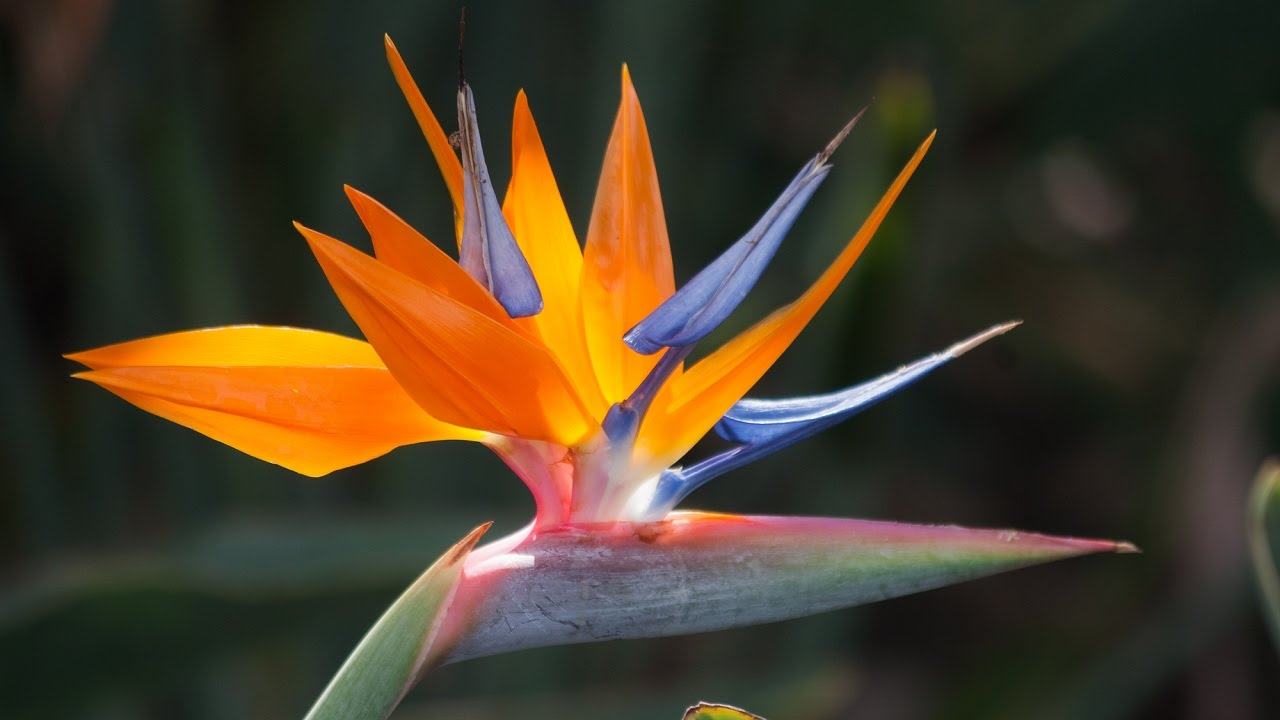
\includegraphics[max width=0.95\textwidth,max height=0.7\textheight]{{Images/bop}.jpg}
\end{center}
\end{column}
\end{columns}
\end{frame}
\subsection*{Q2}
\begin{frame}[t]{Round 1 --- Flowers --- \mbox{Question 2}}
\vspace{-0.5em}
\begin{block}{Question}
``Tulip mania'' was the name given to which country's craze --- that ended in a spectacular crash in 1637 --- for tulip bulbs?
\end{block}
\end{frame}
\subsection*{Q3}
\begin{frame}[t]{Round 1 --- Flowers --- \mbox{Question 3}}
\vspace{-0.5em}
\begin{block}{Question}
Flowers are the reproductive body of flowering plants. Once  fertilized, what do flowering plants begin to produce?
\end{block}
\end{frame}
\subsection*{Q4}
\begin{frame}[t]{Round 1 --- Flowers --- \mbox{Question 4}}
\vspace{-0.5em}
\begin{block}{Question}
After the Chernobyl disaster, what kind of flower was planted in large numbers in the surrounding area to soak up radioactive metals, thereby becoming an international symbol of denuclearization?
\end{block}
\end{frame}
\subsection*{Q5}
\begin{frame}[t]{Round 1 --- Flowers --- \mbox{Question 5}}
\vspace{-0.5em}
\begin{columns}[T,totalwidth=\linewidth]
\begin{column}{0.32\linewidth}
\begin{block}{Question}
In order to attract flies to pollinate it, the titan arum flower --- pictured here --- emits a smell similar to rotting flesh. What more colloquial name is this flower also known by?
\end{block}
\end{column}
\begin{column}{0.65\linewidth}
\begin{center}
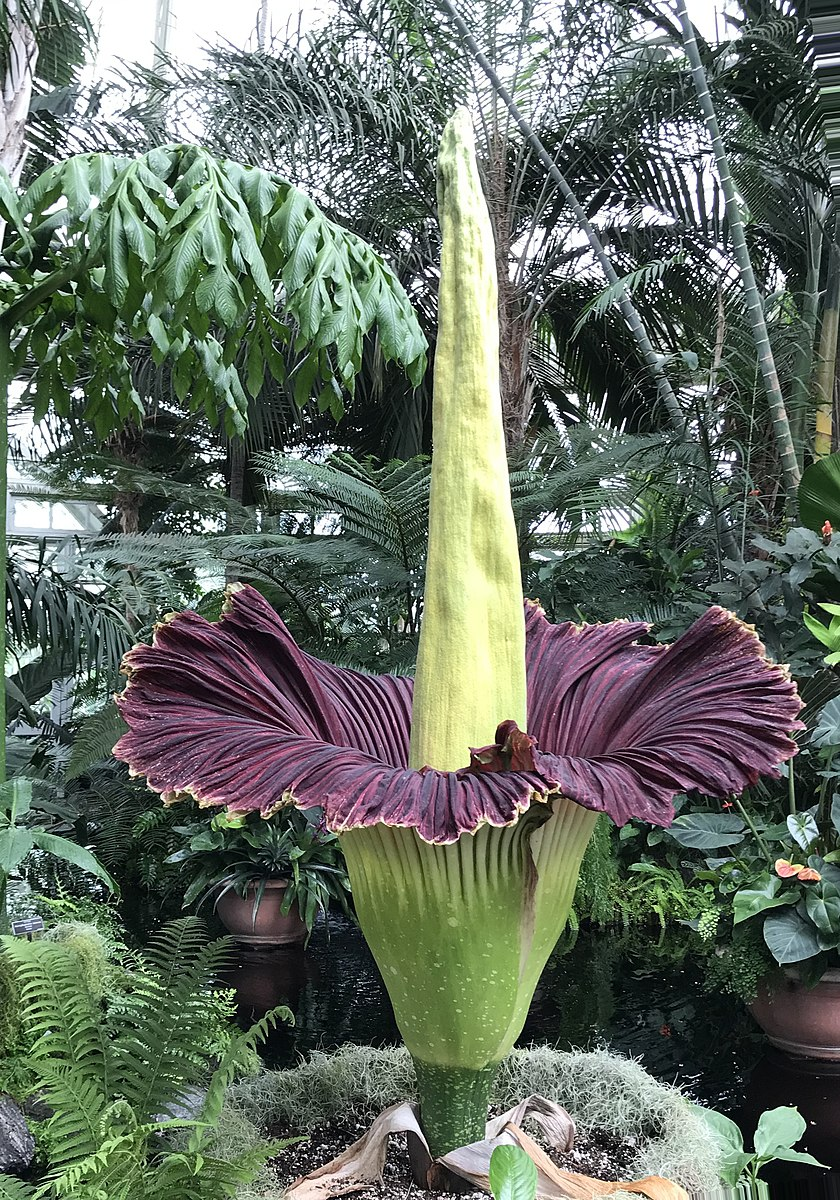
\includegraphics[max width=0.95\textwidth,max height=0.7\textheight]{{Images/corpse}.jpg}
\end{center}
\end{column}
\end{columns}
\end{frame}
\subsection*{Q6}
\begin{frame}[t]{Round 1 --- Flowers --- \mbox{Question 6}}
\vspace{-0.5em}
\begin{block}{Question}
What kind of flower is saffron produced from?
\end{block}
\end{frame}
\subsection*{Q7}
\begin{frame}[t]{Round 1 --- Flowers --- \mbox{Question 7}}
\vspace{-0.5em}
\begin{columns}[T,totalwidth=\linewidth]
\begin{column}{0.32\linewidth}
\begin{block}{Question}
What is the name of the orange flower parts pictured here, which contain the flower's pollen?
\end{block}
\end{column}
\begin{column}{0.65\linewidth}
\begin{center}
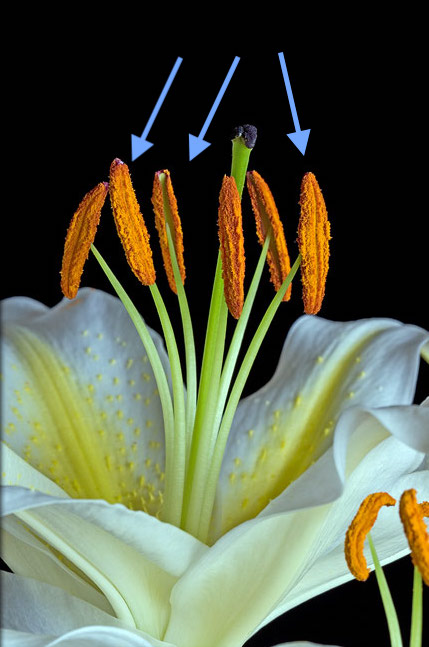
\includegraphics[max width=0.95\textwidth,max height=0.7\textheight]{{Images/anther}.jpg}
\end{center}
\end{column}
\end{columns}
\end{frame}
\subsection*{Q8}
\begin{frame}[t]{Round 1 --- Flowers --- \mbox{Question 8}}
\vspace{-0.5em}
\begin{block}{Question}
What kind of flower is an important symbol in Hinduism and Buddhism and is the national flower of India and Nepal?
\end{block}
\end{frame}
\subsection*{Q9}
\begin{frame}[t]{Round 1 --- Flowers --- \mbox{Question 9}}
\vspace{-0.5em}
\begin{block}{Question}
What kind of plant, which blooms only once or twice per century, exhibits ``mass flowering'' --- a phenomenon in which all plants bloom at the same time --- and holds the record for the most time between blooms at 130 years?
\end{block}
\end{frame}
\subsection*{Q10}
\begin{frame}[t]{Round 1 --- Flowers --- \mbox{Question 10}}
\vspace{-0.5em}
\begin{block}{Question}
What is the national flower (or, more precisely, the national floral emblem) of the U.S.?
\end{block}
\end{frame}
\subsection{Answers}
\begin{frame}[t]{Round 1 --- Flowers --- \mbox{Answer 1}}
\vspace{-0.5em}
\begin{columns}[T,totalwidth=\linewidth]
\begin{column}{0.32\linewidth}
\begin{block}{Question}
What kind of flower is pictured here?
\end{block}
\visible<2->{
    \begin{block}{Answer}
    A bird of paradise
    \end{block}
}
\end{column}
\begin{column}{0.65\linewidth}
\begin{center}
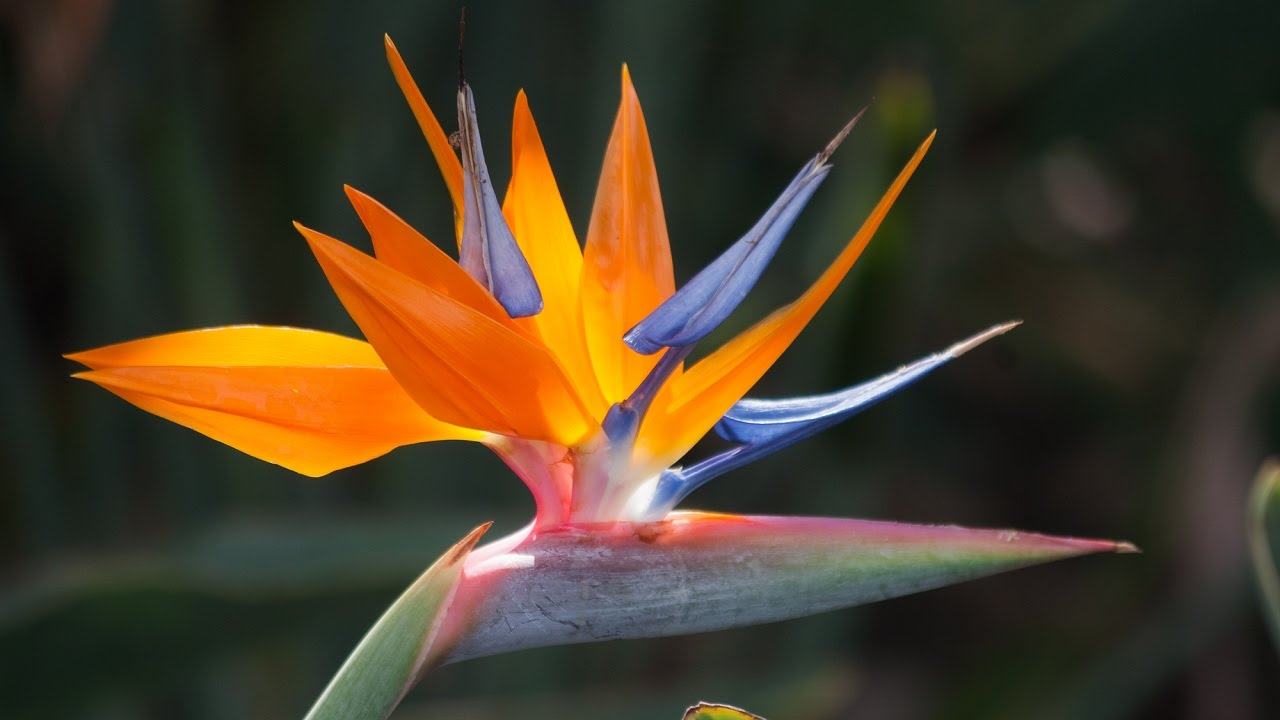
\includegraphics[max width=0.95\textwidth,max height=0.7\textheight]{{Images/bop}.jpg}
\end{center}
\end{column}
\end{columns}
\end{frame}
\begin{frame}[t]{Round 1 --- Flowers --- \mbox{Answer 2}}
\vspace{-0.5em}
\begin{block}{Question}
``Tulip mania'' was the name given to which country's craze --- that ended in a spectacular crash in 1637 --- for tulip bulbs?
\end{block}

\visible<2->{
    \begin{columns}[T,totalwidth=\linewidth]
    \begin{column}{0.32\linewidth}
    \begin{block}{Answer}
    Holland / the Netherlands
    \end{block}
    \end{column}
    \begin{column}{0.65\linewidth}
    \begin{center}
    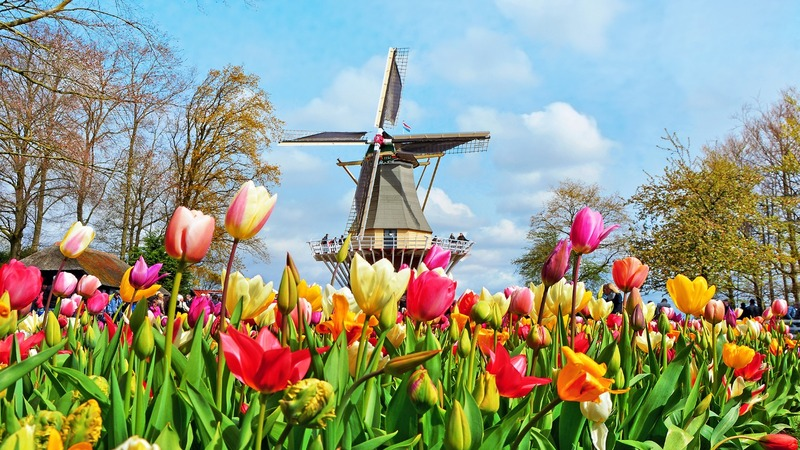
\includegraphics[max width=0.95\textwidth,
        max height=0.50000\textheight]{{Images/tulip}.jpg}
    \end{center}
    \end{column}
    \end{columns}
}
\end{frame}
\begin{frame}[t]{Round 1 --- Flowers --- \mbox{Answer 3}}
\vspace{-0.5em}
\begin{block}{Question}
Flowers are the reproductive body of flowering plants. Once  fertilized, what do flowering plants begin to produce?
\end{block}

\visible<2->{
    \begin{columns}[T,totalwidth=\linewidth]
    \begin{column}{0.32\linewidth}
    \begin{block}{Answer}
    Fruit
    \end{block}
    \end{column}
    \begin{column}{0.65\linewidth}
    \begin{center}
    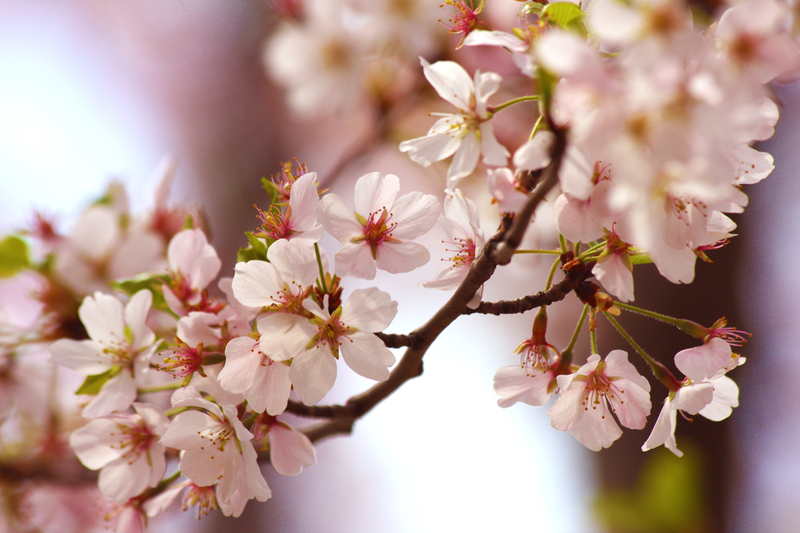
\includegraphics[max width=0.95\textwidth,
        max height=0.50000\textheight]{{Images/cherryblossom}.jpg}
    \end{center}
    \end{column}
    \end{columns}
}
\end{frame}
\begin{frame}[t]{Round 1 --- Flowers --- \mbox{Answer 4}}
\vspace{-0.5em}
\begin{block}{Question}
After the Chernobyl disaster, what kind of flower was planted in large numbers in the surrounding area to soak up radioactive metals, thereby becoming an international symbol of denuclearization?
\end{block}

\visible<2->{
    \begin{columns}[T,totalwidth=\linewidth]
    \begin{column}{0.32\linewidth}
    \begin{block}{Answer}
    Sunflowers
    \end{block}
    \end{column}
    \begin{column}{0.65\linewidth}
    \begin{center}
    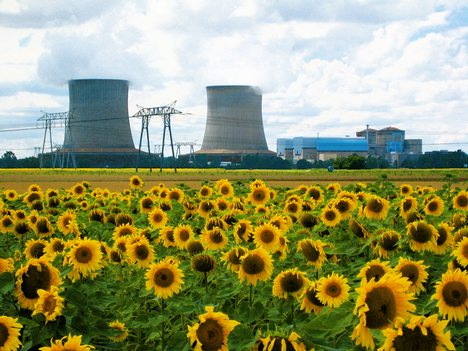
\includegraphics[max width=0.95\textwidth,
        max height=0.46000\textheight]{{Images/sunflower}.jpg}
    \end{center}
    \end{column}
    \end{columns}
}
\end{frame}
\begin{frame}[t]{Round 1 --- Flowers --- \mbox{Answer 5}}
\vspace{-0.5em}
\begin{columns}[T,totalwidth=\linewidth]
\begin{column}{0.32\linewidth}
\begin{block}{Question}
In order to attract flies to pollinate it, the titan arum flower --- pictured here --- emits a smell similar to rotting flesh. What more colloquial name is this flower also known by?
\end{block}
\visible<2->{
    \begin{block}{Answer}
    The corpse flower
    \end{block}
}
\end{column}
\begin{column}{0.65\linewidth}
\begin{center}
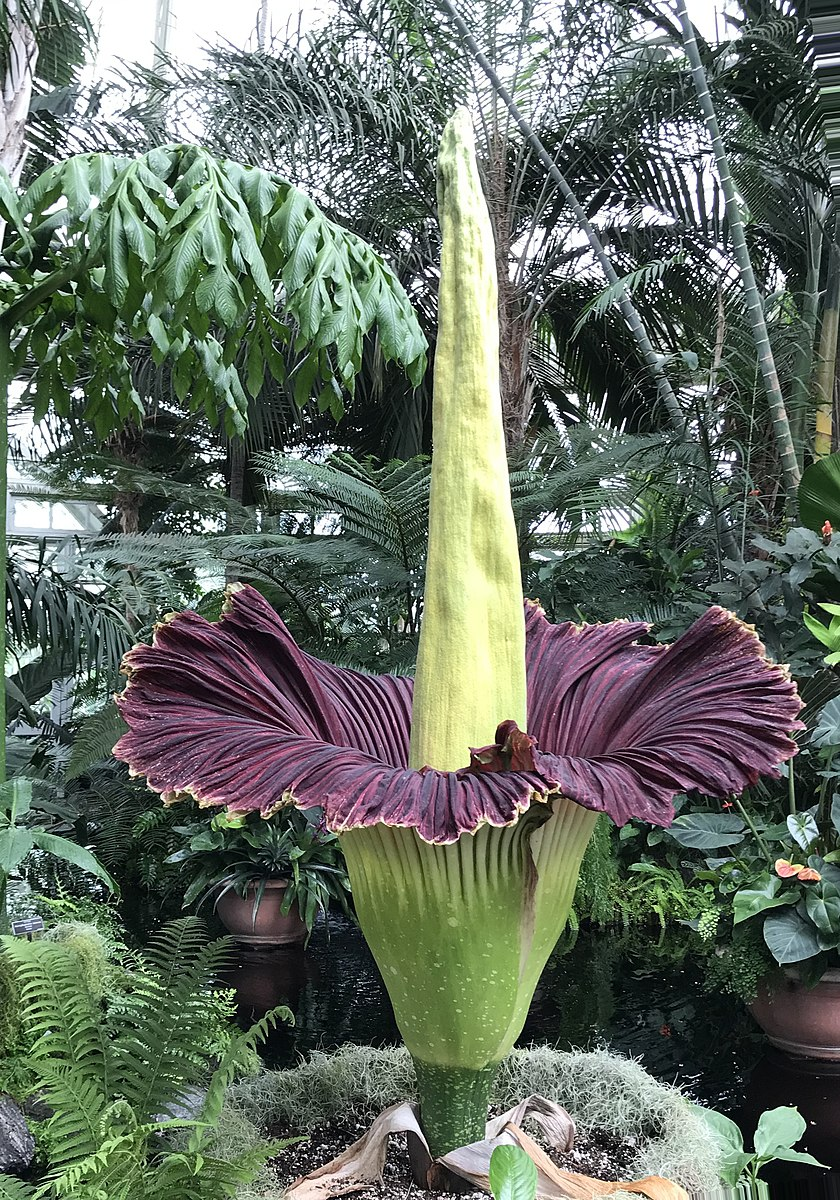
\includegraphics[max width=0.95\textwidth,max height=0.7\textheight]{{Images/corpse}.jpg}
\end{center}
\end{column}
\end{columns}
\end{frame}
\begin{frame}[t]{Round 1 --- Flowers --- \mbox{Answer 6}}
\vspace{-0.5em}
\begin{block}{Question}
What kind of flower is saffron produced from?
\end{block}

\visible<2->{
    \begin{columns}[T,totalwidth=\linewidth]
    \begin{column}{0.32\linewidth}
    \begin{block}{Answer}
    Crocus / autumn crocus / saffron crocus
    \end{block}
    \end{column}
    \begin{column}{0.65\linewidth}
    \begin{center}
    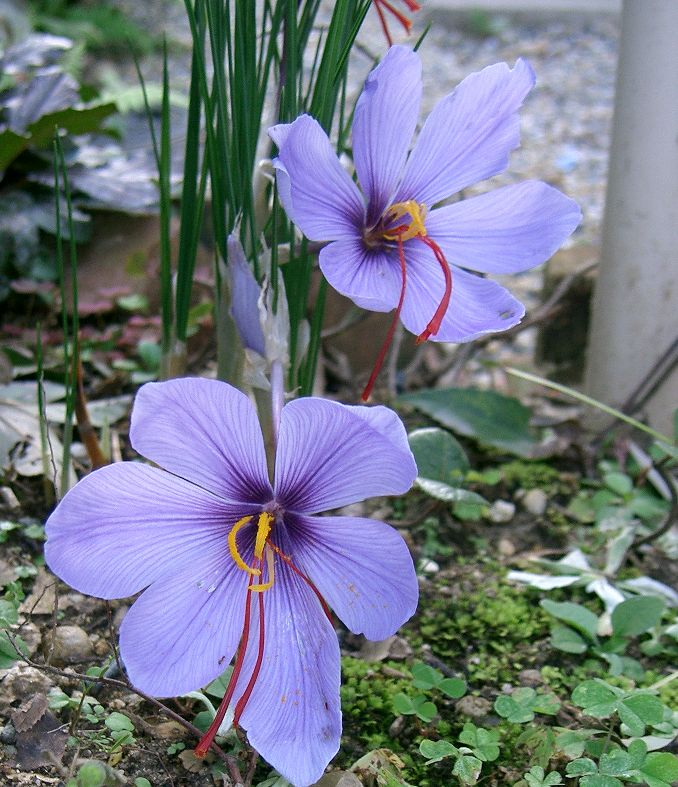
\includegraphics[max width=0.95\textwidth,
        max height=0.58000\textheight]{{Images/crocus}.jpg}
    \end{center}
    \end{column}
    \end{columns}
}
\end{frame}
\begin{frame}[t]{Round 1 --- Flowers --- \mbox{Answer 7}}
\vspace{-0.5em}
\begin{columns}[T,totalwidth=\linewidth]
\begin{column}{0.32\linewidth}
\begin{block}{Question}
What is the name of the orange flower parts pictured here, which contain the flower's pollen?
\end{block}
\visible<2->{
    \begin{block}{Answer}
    Anthers
    \end{block}
}
\end{column}
\begin{column}{0.65\linewidth}
\begin{center}
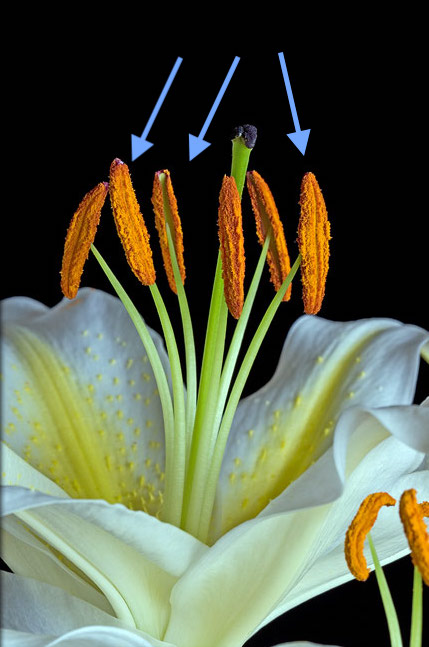
\includegraphics[max width=0.95\textwidth,max height=0.7\textheight]{{Images/anther}.jpg}
\end{center}
\end{column}
\end{columns}
\end{frame}
\begin{frame}[t]{Round 1 --- Flowers --- \mbox{Answer 8}}
\vspace{-0.5em}
\begin{block}{Question}
What kind of flower is an important symbol in Hinduism and Buddhism and is the national flower of India and Nepal?
\end{block}

\visible<2->{
    \begin{columns}[T,totalwidth=\linewidth]
    \begin{column}{0.32\linewidth}
    \begin{block}{Answer}
    The lotus
    \end{block}
    \end{column}
    \begin{column}{0.65\linewidth}
    \begin{center}
    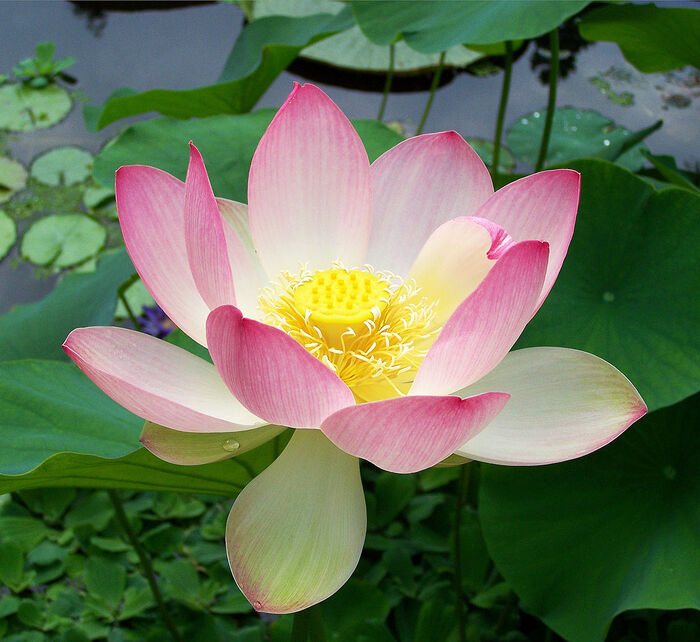
\includegraphics[max width=0.95\textwidth,
        max height=0.50000\textheight]{{Images/lotus}.jpg}
    \end{center}
    \end{column}
    \end{columns}
}
\end{frame}
\begin{frame}[t]{Round 1 --- Flowers --- \mbox{Answer 9}}
\vspace{-0.5em}
\begin{block}{Question}
What kind of plant, which blooms only once or twice per century, exhibits ``mass flowering'' --- a phenomenon in which all plants bloom at the same time --- and holds the record for the most time between blooms at 130 years?
\end{block}

\visible<2->{
    \begin{columns}[T,totalwidth=\linewidth]
    \begin{column}{0.32\linewidth}
    \begin{block}{Answer}
    Bamboo
    \end{block}
    \end{column}
    \begin{column}{0.65\linewidth}
    \begin{center}
    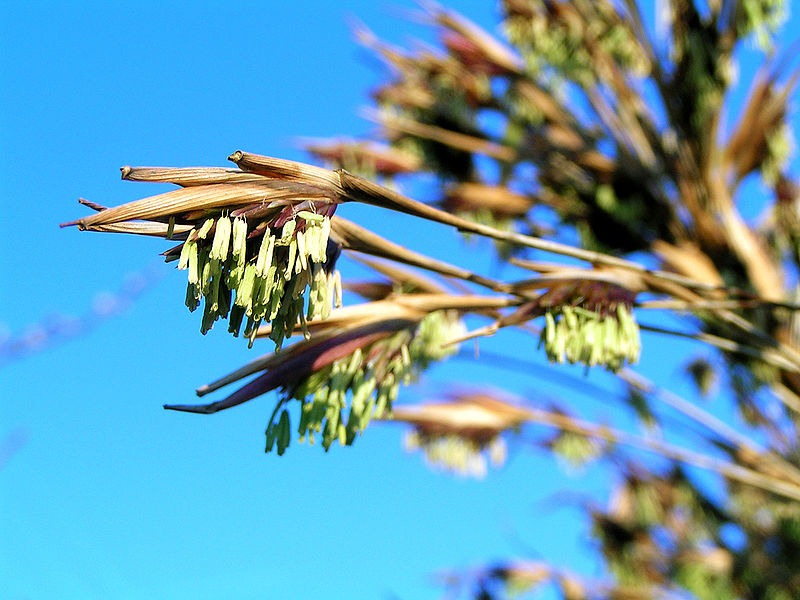
\includegraphics[max width=0.95\textwidth,
        max height=0.42000\textheight]{{Images/bamboo}.jpg}
    \end{center}
    \end{column}
    \end{columns}
}
\end{frame}
\begin{frame}[t]{Round 1 --- Flowers --- \mbox{Answer 10}}
\vspace{-0.5em}
\begin{block}{Question}
What is the national flower (or, more precisely, the national floral emblem) of the U.S.?
\end{block}

\visible<2->{
    \begin{columns}[T,totalwidth=\linewidth]
    \begin{column}{0.32\linewidth}
    \begin{block}{Answer}
    The rose
    \end{block}
    \end{column}
    \begin{column}{0.65\linewidth}
    \begin{center}
    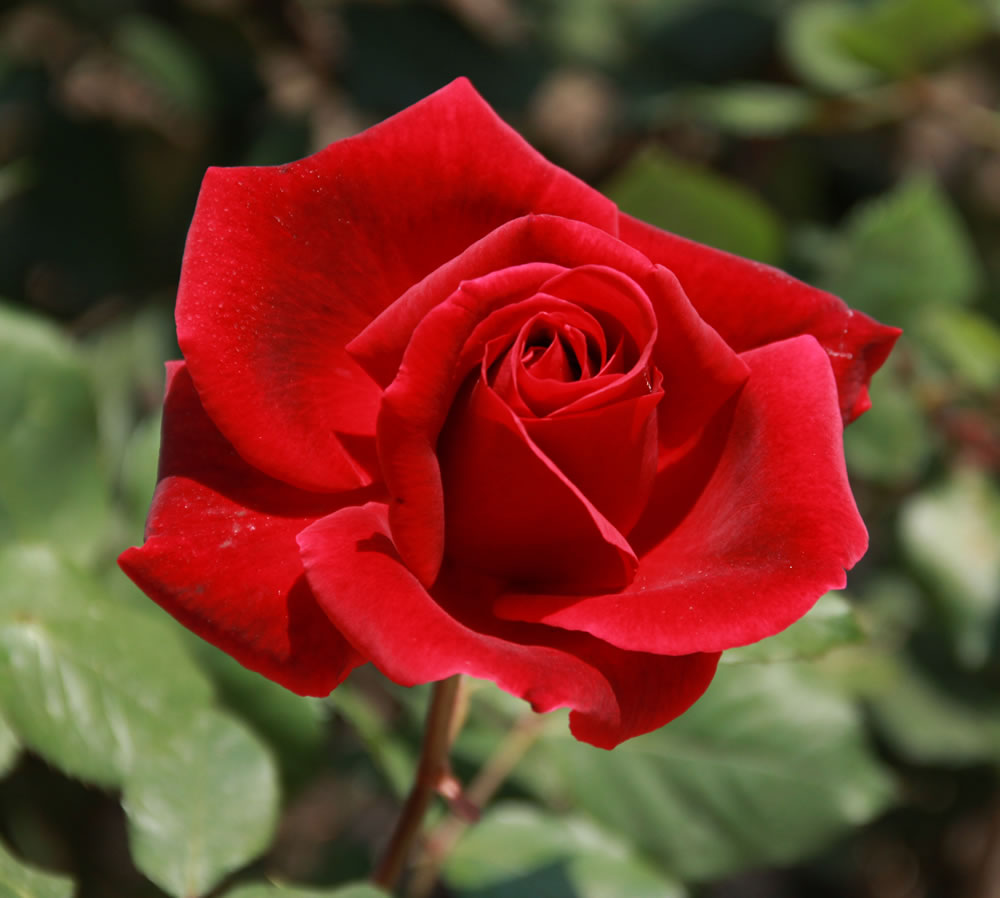
\includegraphics[max width=0.95\textwidth,
        max height=0.54000\textheight]{{Images/rose}.jpg}
    \end{center}
    \end{column}
    \end{columns}
}
\end{frame}
\def\thisSectionName{Abraham Lincoln}
\section{Round 2}
\subsection*{Q1}
\begin{frame}[t]{Round 2 --- Abraham Lincoln --- \mbox{Question 1}}
\vspace{-0.5em}
\begin{block}{Question}
In which state was Lincoln born?
\end{block}
\end{frame}
\subsection*{Q2}
\begin{frame}[t]{Round 2 --- Abraham Lincoln --- \mbox{Question 2}}
\vspace{-0.5em}
\begin{block}{Question}
How many children did Lincoln have?
\end{block}
\end{frame}
\subsection*{Q3}
\begin{frame}[t]{Round 2 --- Abraham Lincoln --- \mbox{Question 3}}
\vspace{-0.5em}
\begin{block}{Question}
In 1849, Lincoln was awarded U.S. patent no.\ 6,469.  What was the patent for?
\end{block}
\end{frame}
\subsection*{Q4}
\begin{frame}[t]{Round 2 --- Abraham Lincoln --- \mbox{Question 4}}
\vspace{-0.5em}
\begin{block}{Question}
Which book by John Bunyan was one of Lincoln's favorites?
\end{block}
\end{frame}
\subsection*{Q5}
\begin{frame}[t]{Round 2 --- Abraham Lincoln --- \mbox{Question 5}}
\vspace{-0.5em}
\begin{block}{Question}
What elected offices did Lincoln hold before he became president? (We need all of them.)
\end{block}
\end{frame}
\subsection*{Q6}
\begin{frame}[t]{Round 2 --- Abraham Lincoln --- \mbox{Question 6}}
\vspace{-0.5em}
\begin{block}{Question}
What was the name of the 11 year-old girl whose letter to Lincoln encouraging him to grow a beard was acted on by Lincoln?
\end{block}
\end{frame}
\subsection*{Q7}
\begin{frame}[t]{Round 2 --- Abraham Lincoln --- \mbox{Question 7}}
\vspace{-0.5em}
\begin{block}{Question}
What was the maiden name of Lincoln's wife, Mary?
\end{block}
\end{frame}
\subsection*{Q8}
\begin{frame}[t]{Round 2 --- Abraham Lincoln --- \mbox{Question 8}}
\vspace{-0.5em}
\begin{block}{Question}
Who was Lincoln's Vice President in his first term? 
\end{block}
\end{frame}
\subsection*{Q9}
\begin{frame}[t]{Round 2 --- Abraham Lincoln --- \mbox{Question 9}}
\vspace{-0.5em}
\begin{block}{Question}
On what date (month, day and year) was Lincoln assassinated, and on what date did he die? (We need both dates.)
\end{block}
\end{frame}
\subsection*{Q10}
\begin{frame}[t]{Round 2 --- Abraham Lincoln --- \mbox{Question 10}}
\vspace{-0.5em}
\begin{block}{Question}
Lincoln's Secretary of War, Edwin Stanton, was present at Lincoln's deathbed when Lincoln died.  What are the  famous words that Secretary Stanton was reported to have said in the moment after the doctor declared Lincoln dead?
\end{block}
\end{frame}
\subsection{Answers}
\begin{frame}[t]{Round 2 --- Abraham Lincoln --- \mbox{Answer 1}}
\vspace{-0.5em}
\begin{block}{Question}
In which state was Lincoln born?
\end{block}

\visible<2->{
    \begin{columns}[T,totalwidth=\linewidth]
    \begin{column}{0.32\linewidth}
    \begin{block}{Answer}
    Kentucky
    \end{block}
    \end{column}
    \begin{column}{0.65\linewidth}
    \begin{center}
    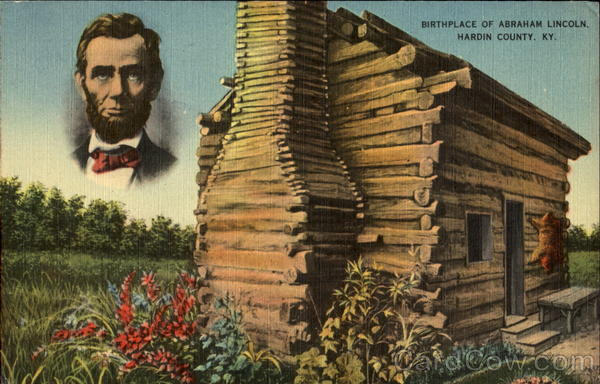
\includegraphics[max width=0.95\textwidth,
        max height=0.58000\textheight]{{Images/kentucky}.jpg}
    \end{center}
    \end{column}
    \end{columns}
}
\end{frame}
\begin{frame}[t]{Round 2 --- Abraham Lincoln --- \mbox{Answer 2}}
\vspace{-0.5em}
\begin{block}{Question}
How many children did Lincoln have?
\end{block}

\visible<2->{
    \begin{columns}[T,totalwidth=\linewidth]
    \begin{column}{0.32\linewidth}
    \begin{block}{Answer}
    Four (all sons)
    \end{block}
    \end{column}
    \begin{column}{0.65\linewidth}
    \begin{center}
    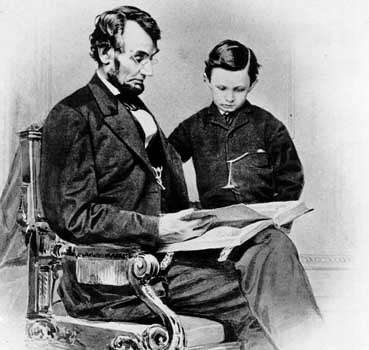
\includegraphics[max width=0.95\textwidth,
        max height=0.58000\textheight]{{Images/lincolnson}.jpg}
    \end{center}
    \end{column}
    \end{columns}
}
\end{frame}
\begin{frame}[t]{Round 2 --- Abraham Lincoln --- \mbox{Answer 3}}
\vspace{-0.5em}
\begin{block}{Question}
In 1849, Lincoln was awarded U.S. patent no.\ 6,469.  What was the patent for?
\end{block}

\visible<2->{
    \begin{columns}[T,totalwidth=\linewidth]
    \begin{column}{0.32\linewidth}
    \begin{block}{Answer}
    A method for keeping vessels afloat when traversing shallow waters through the use of empty metal air chambers attached to their sides.
    \end{block}
    \end{column}
    \begin{column}{0.65\linewidth}
    \begin{center}
    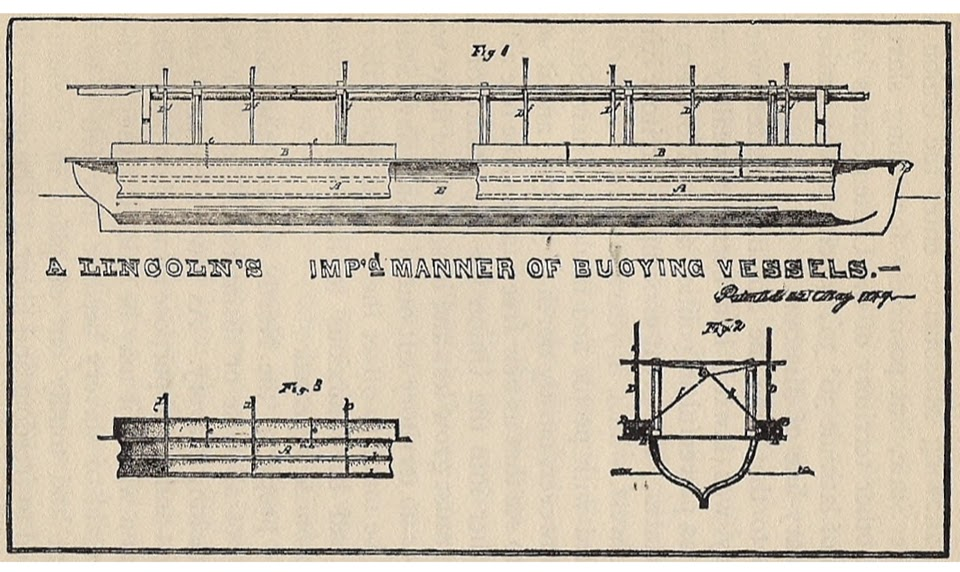
\includegraphics[max width=0.95\textwidth,
        max height=0.54000\textheight]{{Images/patent}.jpg}
    \end{center}
    \end{column}
    \end{columns}
}
\end{frame}
\begin{frame}[t]{Round 2 --- Abraham Lincoln --- \mbox{Answer 4}}
\vspace{-0.5em}
\begin{block}{Question}
Which book by John Bunyan was one of Lincoln's favorites?
\end{block}

\visible<2->{
    \begin{columns}[T,totalwidth=\linewidth]
    \begin{column}{0.32\linewidth}
    \begin{block}{Answer}
    \emph{The Pilgrim's Progress}
    \end{block}
    \end{column}
    \begin{column}{0.65\linewidth}
    \begin{center}
    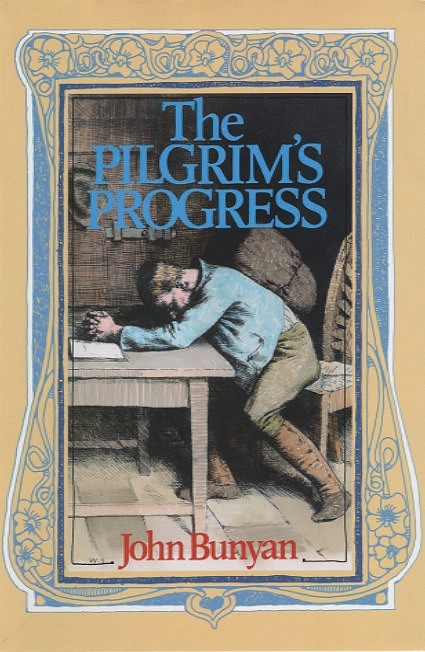
\includegraphics[max width=0.95\textwidth,
        max height=0.54000\textheight]{{Images/pilgrim}.jpg}
    \end{center}
    \end{column}
    \end{columns}
}
\end{frame}
\begin{frame}[t]{Round 2 --- Abraham Lincoln --- \mbox{Answer 5}}
\vspace{-0.5em}
\begin{block}{Question}
What elected offices did Lincoln hold before he became president? (We need all of them.)
\end{block}

\visible<2->{
    \begin{columns}[T,totalwidth=\linewidth]
    \begin{column}{0.32\linewidth}
    \begin{block}{Answer}
    Member of the Illinois House of Representatives and Congressman
    \end{block}
    \end{column}
    \begin{column}{0.65\linewidth}
    \begin{center}
    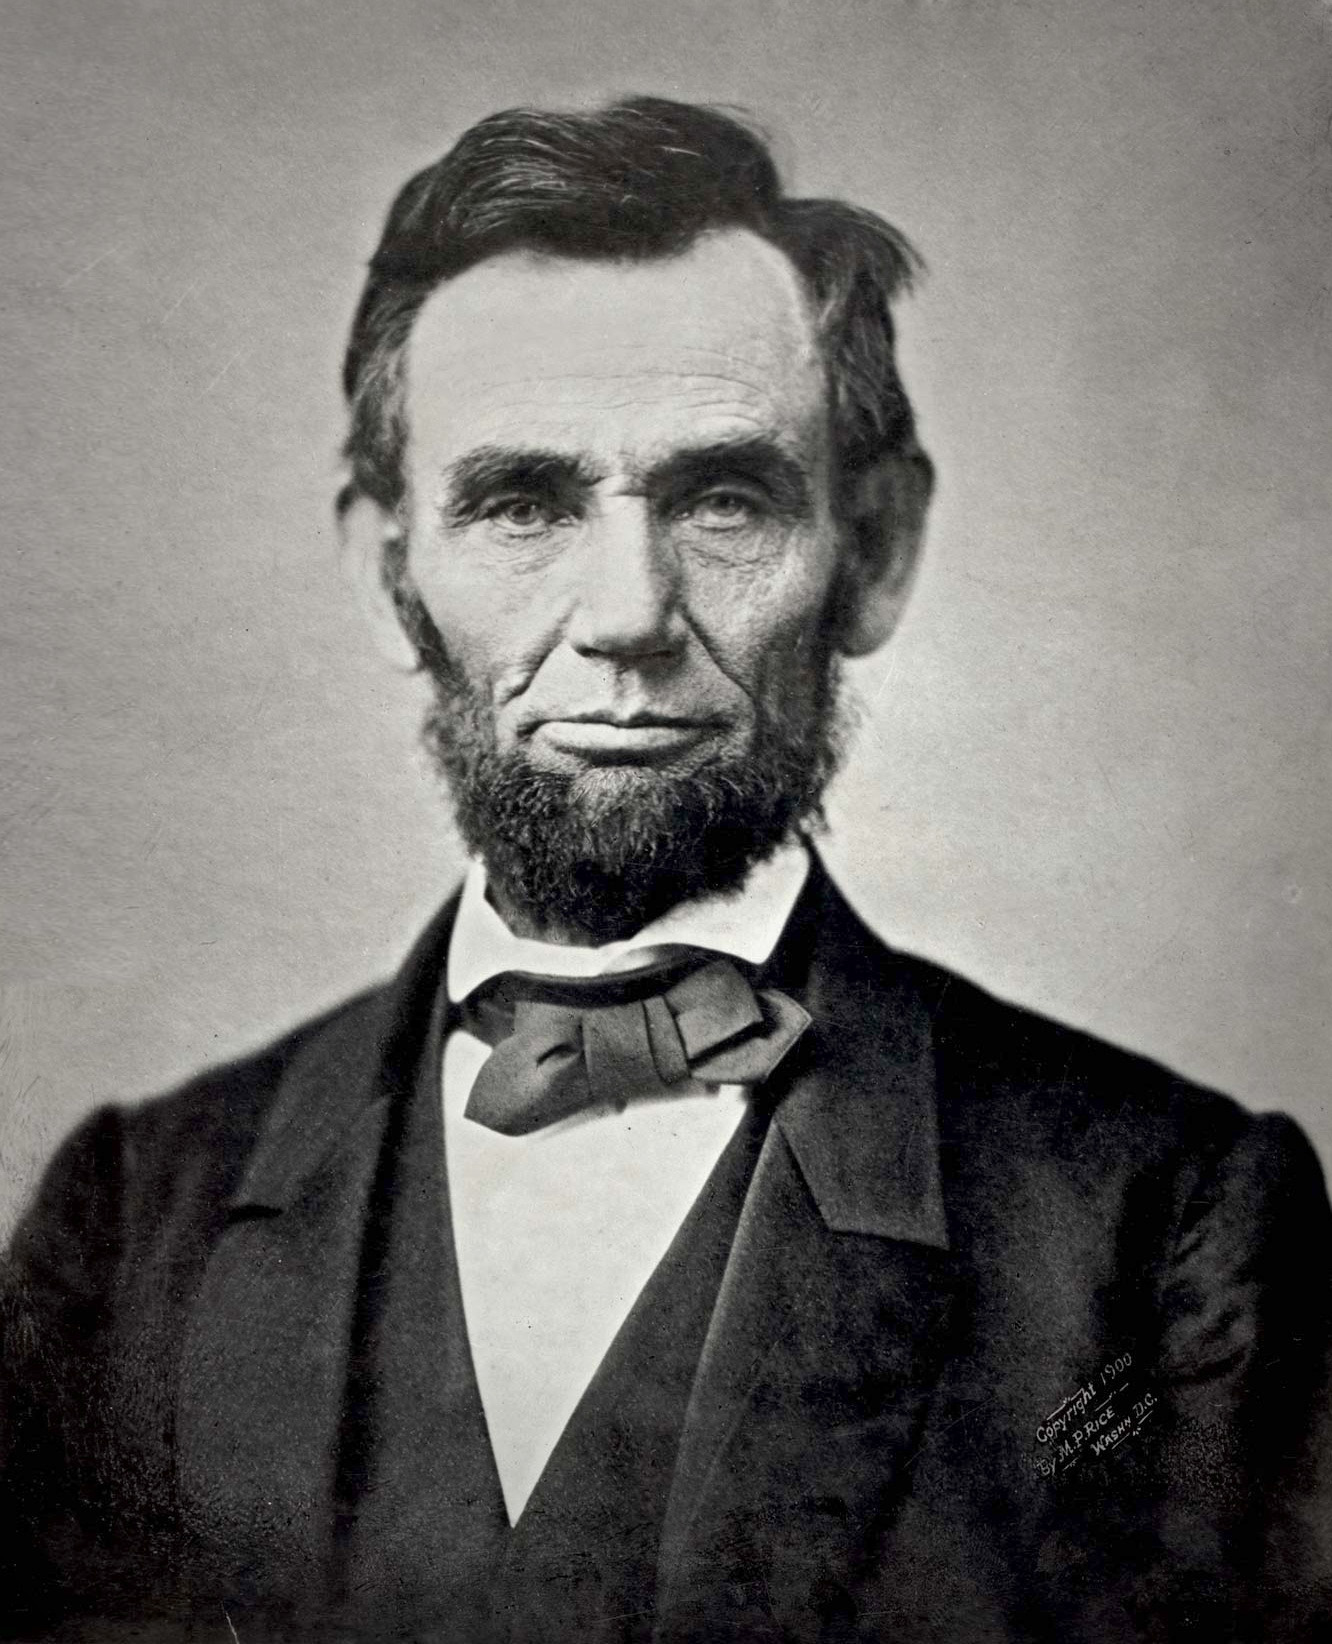
\includegraphics[max width=0.95\textwidth,
        max height=0.54000\textheight]{{Images/lincoln}.jpg}
    \end{center}
    \end{column}
    \end{columns}
}
\end{frame}
\begin{frame}[t]{Round 2 --- Abraham Lincoln --- \mbox{Answer 6}}
\vspace{-0.5em}
\begin{block}{Question}
What was the name of the 11 year-old girl whose letter to Lincoln encouraging him to grow a beard was acted on by Lincoln?
\end{block}

\visible<2->{
    \begin{columns}[T,totalwidth=\linewidth]
    \begin{column}{0.32\linewidth}
    \begin{block}{Answer}
    Grace Bedell
    \end{block}
    \end{column}
    \begin{column}{0.65\linewidth}
    \begin{center}
    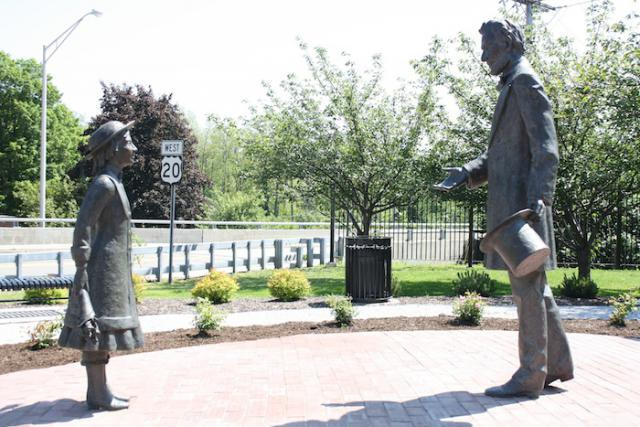
\includegraphics[max width=0.95\textwidth,
        max height=0.50000\textheight]{{Images/bedell}.jpg}
    \end{center}
    \end{column}
    \end{columns}
}
\end{frame}
\begin{frame}[t]{Round 2 --- Abraham Lincoln --- \mbox{Answer 7}}
\vspace{-0.5em}
\begin{block}{Question}
What was the maiden name of Lincoln's wife, Mary?
\end{block}

\visible<2->{
    \begin{columns}[T,totalwidth=\linewidth]
    \begin{column}{0.32\linewidth}
    \begin{block}{Answer}
    Todd
    \end{block}
    \end{column}
    \begin{column}{0.65\linewidth}
    \begin{center}
    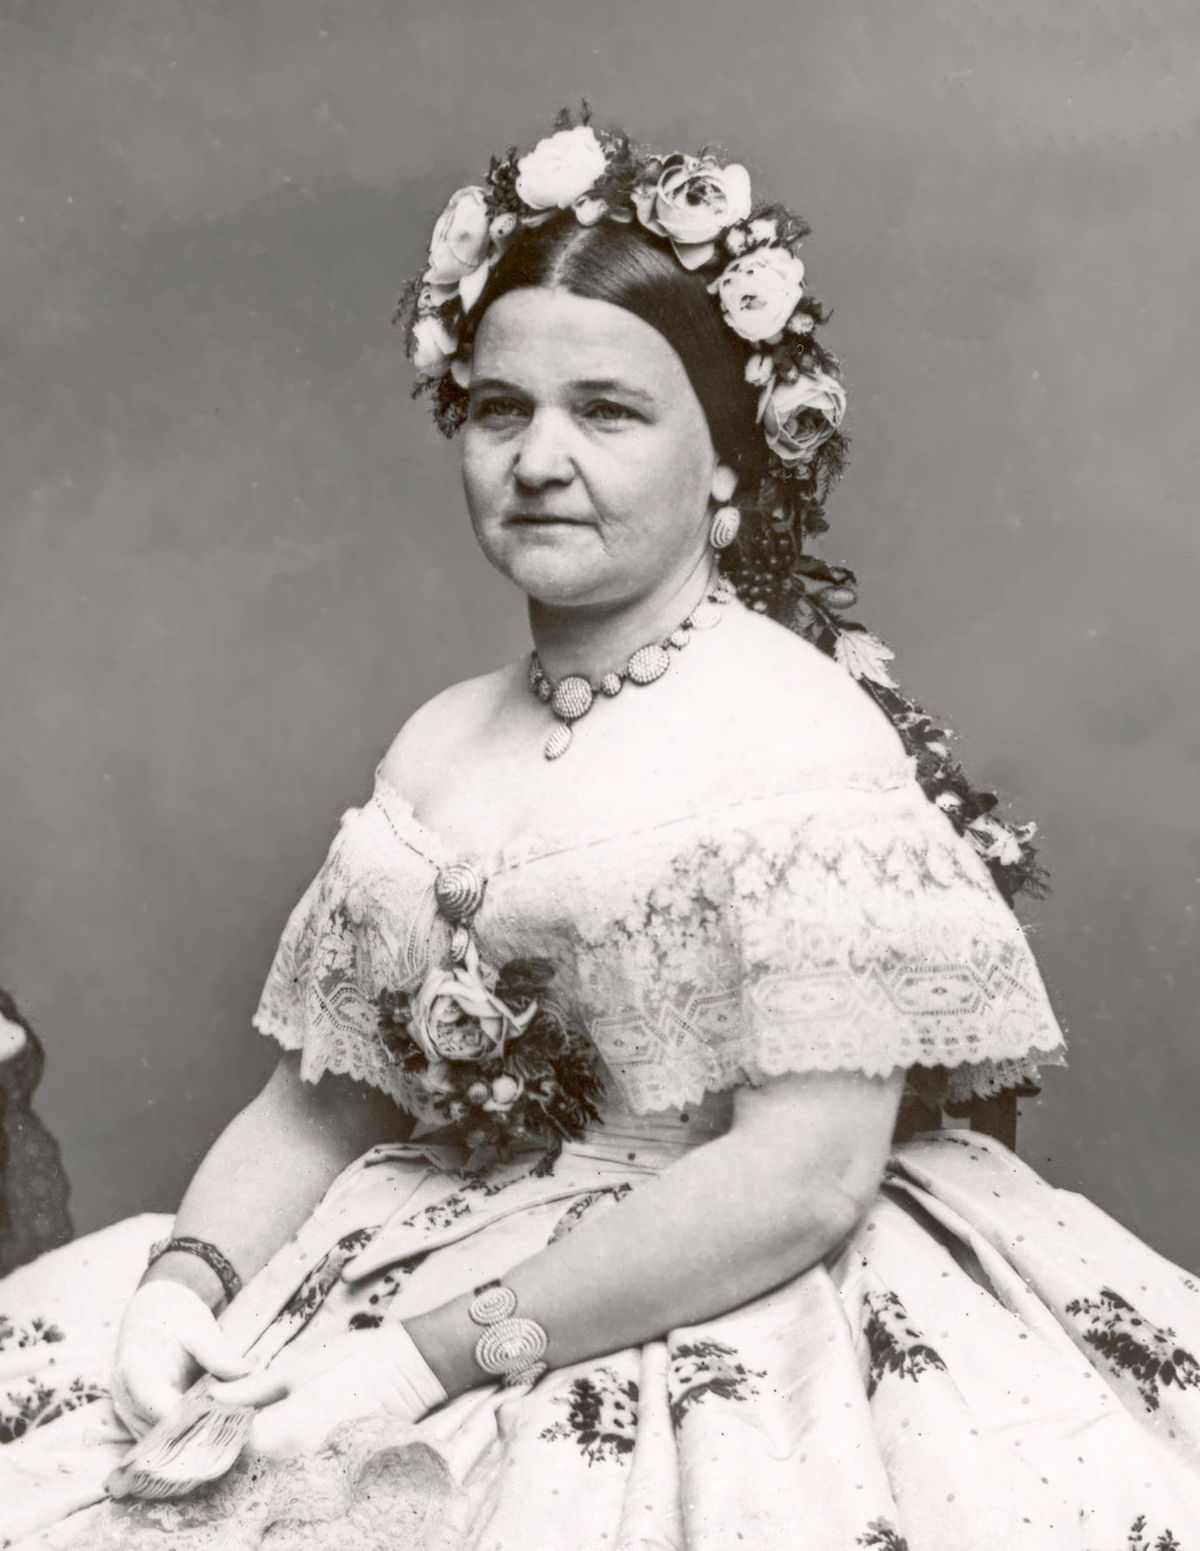
\includegraphics[max width=0.95\textwidth,
        max height=0.58000\textheight]{{Images/marytodd}.jpg}
    \end{center}
    \end{column}
    \end{columns}
}
\end{frame}
\begin{frame}[t]{Round 2 --- Abraham Lincoln --- \mbox{Answer 8}}
\vspace{-0.5em}
\begin{block}{Question}
Who was Lincoln's Vice President in his first term? 
\end{block}

\visible<2->{
    \begin{columns}[T,totalwidth=\linewidth]
    \begin{column}{0.32\linewidth}
    \begin{block}{Answer}
    Hannibal Hamlin
    \end{block}
    \end{column}
    \begin{column}{0.65\linewidth}
    \begin{center}
    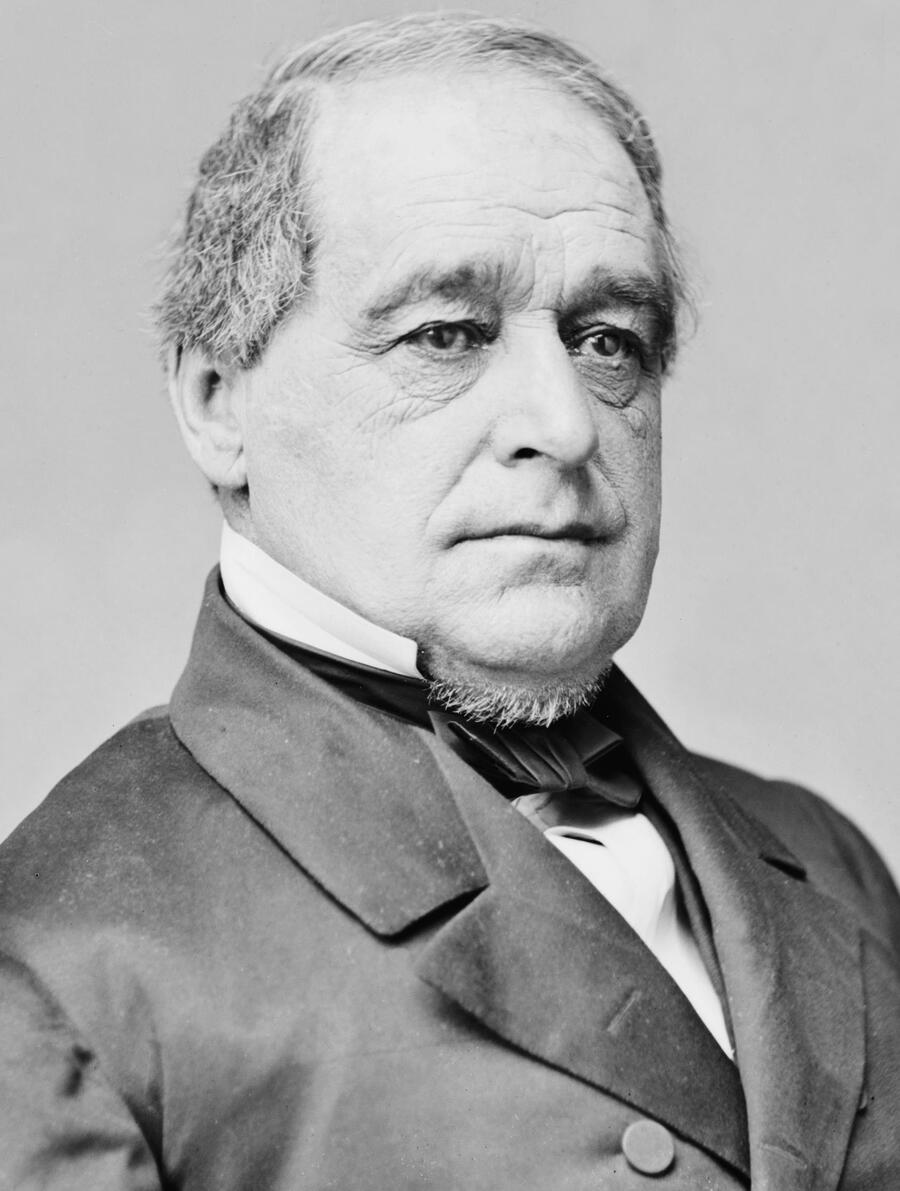
\includegraphics[max width=0.95\textwidth,
        max height=0.54000\textheight]{{Images/hannibalhamlin}.jpg}
    \end{center}
    \end{column}
    \end{columns}
}
\end{frame}
\begin{frame}[t]{Round 2 --- Abraham Lincoln --- \mbox{Answer 9}}
\vspace{-0.5em}
\begin{block}{Question}
On what date (month, day and year) was Lincoln assassinated, and on what date did he die? (We need both dates.)
\end{block}

\visible<2->{
    \begin{columns}[T,totalwidth=\linewidth]
    \begin{column}{0.32\linewidth}
    \begin{block}{Answer}
    Lincoln was assassinated on April 14, 1865, and he died on April 15, 1865.
    \end{block}
    \end{column}
    \begin{column}{0.65\linewidth}
    \begin{center}
    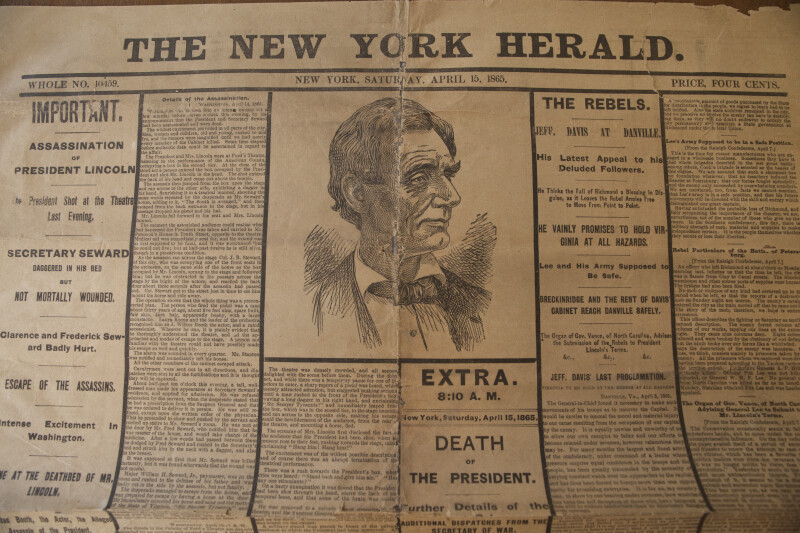
\includegraphics[max width=0.95\textwidth,
        max height=0.50000\textheight]{{Images/lincolnassassinated}.jpg}
    \end{center}
    \end{column}
    \end{columns}
}
\end{frame}
\begin{frame}[t]{Round 2 --- Abraham Lincoln --- \mbox{Answer 10}}
\vspace{-0.5em}
\begin{block}{Question}
Lincoln's Secretary of War, Edwin Stanton, was present at Lincoln's deathbed when Lincoln died.  What are the  famous words that Secretary Stanton was reported to have said in the moment after the doctor declared Lincoln dead?
\end{block}

\visible<2->{
    \begin{columns}[T,totalwidth=\linewidth]
    \begin{column}{0.32\linewidth}
    \begin{block}{Answer}
    ``Now he belongs to the ages.''
    \end{block}
    \end{column}
    \begin{column}{0.65\linewidth}
    \begin{center}
    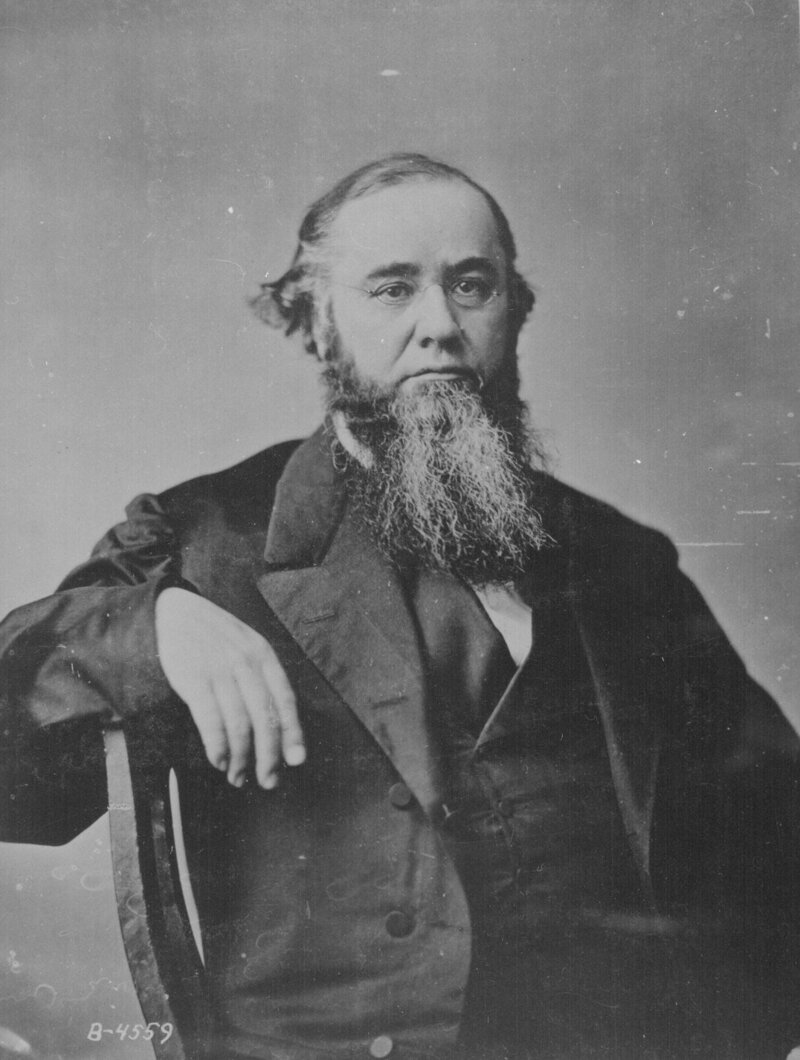
\includegraphics[max width=0.95\textwidth,
        max height=0.42000\textheight]{{Images/stanton}.jpg}
    \end{center}
    \end{column}
    \end{columns}
}
\end{frame}
\def\thisSectionName{Civil Rights Movements}
\section{Round 3}
\subsection*{Q1}
\begin{frame}[t]{Round 3 --- Civil Rights Movements --- \mbox{Question 1}}
\vspace{-0.5em}
\begin{block}{Question}
Name the civil rights activist who was the Field Secretary for the Mississippi NAACP and who was assassinated on June 12, 1963.
\end{block}
\end{frame}
\subsection*{Q2}
\begin{frame}[t]{Round 3 --- Civil Rights Movements --- \mbox{Question 2}}
\vspace{-0.5em}
\begin{block}{Question}
What year did the Stonewall Riots take place?
\end{block}
\end{frame}
\subsection*{Q3}
\begin{frame}[t]{Round 3 --- Civil Rights Movements --- \mbox{Question 3}}
\vspace{-0.5em}
\begin{block}{Question}
Which amendment to the U.S. Constitution gave women the right to vote?
\end{block}
\end{frame}
\subsection*{Q4}
\begin{frame}[t]{Round 3 --- Civil Rights Movements --- \mbox{Question 4}}
\vspace{-0.5em}
\begin{block}{Question}
Which amendment to the U.S. Constitution gave African-Americans the right to vote?
\end{block}
\end{frame}
\subsection*{Q5}
\begin{frame}[t]{Round 3 --- Civil Rights Movements --- \mbox{Question 5}}
\vspace{-0.5em}
\begin{block}{Question}
What is name of the process that took place in South Africa after the end of apartheid in which those who fostered apartheid faced those they had harmed and admitted what they had done?
\end{block}
\end{frame}
\subsection*{Q6}
\begin{frame}[t]{Round 3 --- Civil Rights Movements --- \mbox{Question 6}}
\vspace{-0.5em}
\begin{block}{Question}
What civil rights group was known by its initials, SNCC\@?
\end{block}
\end{frame}
\subsection*{Q7}
\begin{frame}[t]{Round 3 --- Civil Rights Movements --- \mbox{Question 7}}
\vspace{-0.5em}
\begin{block}{Question}
What is the commodity that Gandhi, in an act of civil disobedience, produced in violation of a monopoly granted by the British government?
\end{block}
\end{frame}
\subsection*{Q8}
\begin{frame}[t]{Round 3 --- Civil Rights Movements --- \mbox{Question 8}}
\vspace{-0.5em}
\begin{block}{Question}
What is the name of the essay in which Martin Luther King argued to fellow clergy that they were wrong in saying that the time was not yet right for action on civil rights?
\end{block}
\end{frame}
\subsection*{Q9}
\begin{frame}[t]{Round 3 --- Civil Rights Movements --- \mbox{Question 9}}
\vspace{-0.5em}
\begin{block}{Question}
What is the name of the woman who was known as the ``The First Lady of the Struggle'' and who was the only African-American woman to be part of the U.S. delegation to the group that created of the United Nations charter?
\end{block}
\end{frame}
\subsection*{Q10}
\begin{frame}[t]{Round 3 --- Civil Rights Movements --- \mbox{Question 10}}
\vspace{-0.5em}
\begin{block}{Question}
What is the name of the woman born in Mississippi in 1862 who became best known for her work as a crusading journalist  who exposed the prevalence and horror  of lynching?
\end{block}
\end{frame}
\subsection{Answers}
\begin{frame}[t]{Round 3 --- Civil Rights Movements --- \mbox{Answer 1}}
\vspace{-0.5em}
\begin{block}{Question}
Name the civil rights activist who was the Field Secretary for the Mississippi NAACP and who was assassinated on June 12, 1963.
\end{block}

\visible<2->{
    \begin{columns}[T,totalwidth=\linewidth]
    \begin{column}{0.32\linewidth}
    \begin{block}{Answer}
    Medgar Evers
    \end{block}
    \end{column}
    \begin{column}{0.65\linewidth}
    \begin{center}
    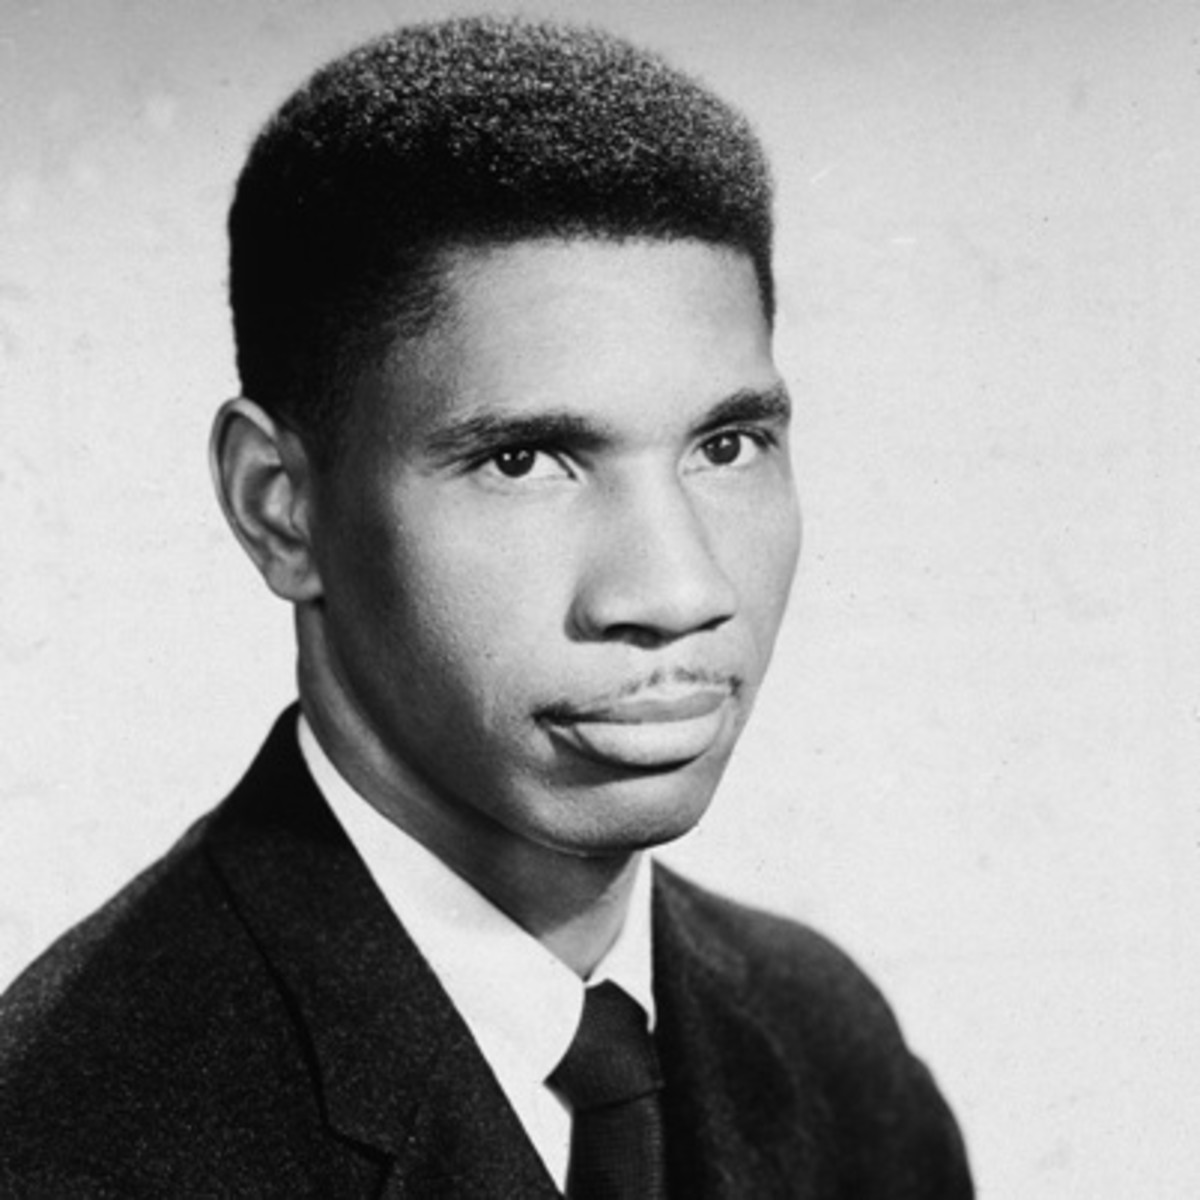
\includegraphics[max width=0.95\textwidth,
        max height=0.50000\textheight]{{Images/evers}.jpg}
    \end{center}
    \end{column}
    \end{columns}
}
\end{frame}
\begin{frame}[t]{Round 3 --- Civil Rights Movements --- \mbox{Answer 2}}
\vspace{-0.5em}
\begin{block}{Question}
What year did the Stonewall Riots take place?
\end{block}

\visible<2->{
    \begin{columns}[T,totalwidth=\linewidth]
    \begin{column}{0.32\linewidth}
    \begin{block}{Answer}
    1969
    \end{block}
    \end{column}
    \begin{column}{0.65\linewidth}
    \begin{center}
    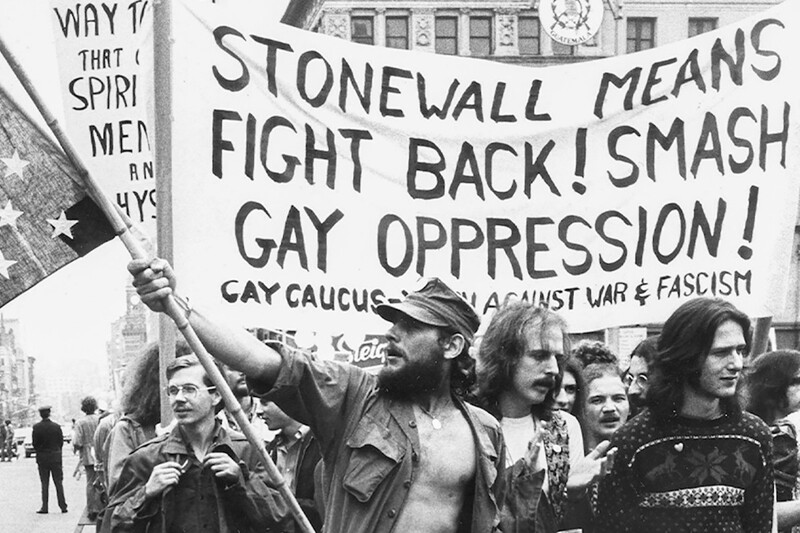
\includegraphics[max width=0.95\textwidth,
        max height=0.58000\textheight]{{Images/stonewall}.jpg}
    \end{center}
    \end{column}
    \end{columns}
}
\end{frame}
\begin{frame}[t]{Round 3 --- Civil Rights Movements --- \mbox{Answer 3}}
\vspace{-0.5em}
\begin{block}{Question}
Which amendment to the U.S. Constitution gave women the right to vote?
\end{block}

\visible<2->{
    \begin{columns}[T,totalwidth=\linewidth]
    \begin{column}{0.32\linewidth}
    \begin{block}{Answer}
    The 19\textsuperscript{th} Amendment
    \end{block}
    \end{column}
    \begin{column}{0.65\linewidth}
    \begin{center}
    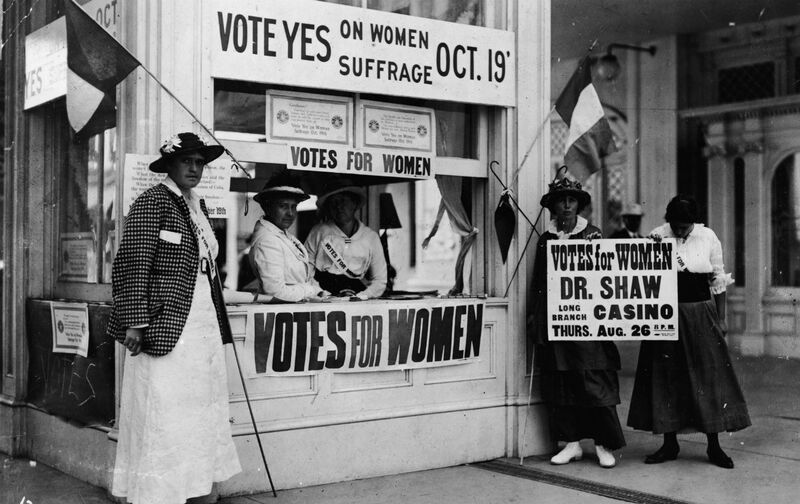
\includegraphics[max width=0.95\textwidth,
        max height=0.54000\textheight]{{Images/amendment19}.jpg}
    \end{center}
    \end{column}
    \end{columns}
}
\end{frame}
\begin{frame}[t]{Round 3 --- Civil Rights Movements --- \mbox{Answer 4}}
\vspace{-0.5em}
\begin{block}{Question}
Which amendment to the U.S. Constitution gave African-Americans the right to vote?
\end{block}

\visible<2->{
    \begin{columns}[T,totalwidth=\linewidth]
    \begin{column}{0.32\linewidth}
    \begin{block}{Answer}
    The 15\textsuperscript{th} Amendment
    \end{block}
    \end{column}
    \begin{column}{0.65\linewidth}
    \begin{center}
    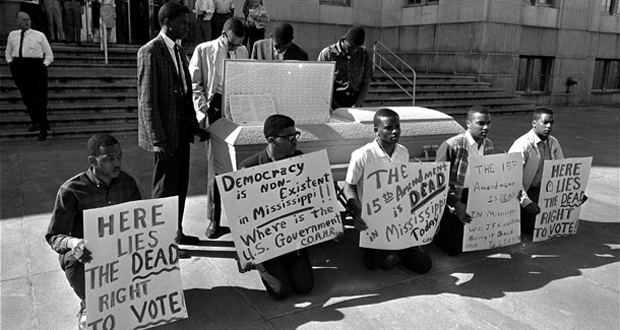
\includegraphics[max width=0.95\textwidth,
        max height=0.54000\textheight]{{Images/amendment15}.jpg}
    \end{center}
    \end{column}
    \end{columns}
}
\end{frame}
\begin{frame}[t]{Round 3 --- Civil Rights Movements --- \mbox{Answer 5}}
\vspace{-0.5em}
\begin{block}{Question}
What is name of the process that took place in South Africa after the end of apartheid in which those who fostered apartheid faced those they had harmed and admitted what they had done?
\end{block}

\visible<2->{
    \begin{columns}[T,totalwidth=\linewidth]
    \begin{column}{0.32\linewidth}
    \begin{block}{Answer}
    Truth and Reconcilation
    \end{block}
    \end{column}
    \begin{column}{0.65\linewidth}
    \begin{center}
    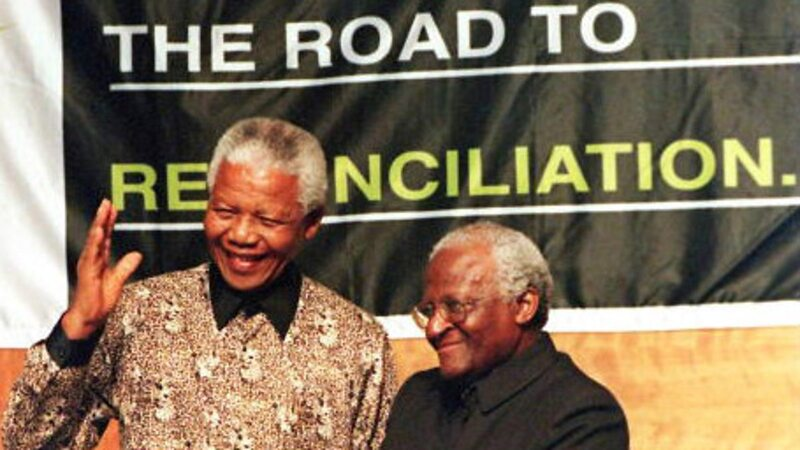
\includegraphics[max width=0.95\textwidth,
        max height=0.46000\textheight]{{Images/reconciliation}.jpg}
    \end{center}
    \end{column}
    \end{columns}
}
\end{frame}
\begin{frame}[t]{Round 3 --- Civil Rights Movements --- \mbox{Answer 6}}
\vspace{-0.5em}
\begin{block}{Question}
What civil rights group was known by its initials, SNCC\@?
\end{block}

\visible<2->{
    \begin{columns}[T,totalwidth=\linewidth]
    \begin{column}{0.32\linewidth}
    \begin{block}{Answer}
    The Student Nonviolent Coordinating Committee
    \end{block}
    \end{column}
    \begin{column}{0.65\linewidth}
    \begin{center}
    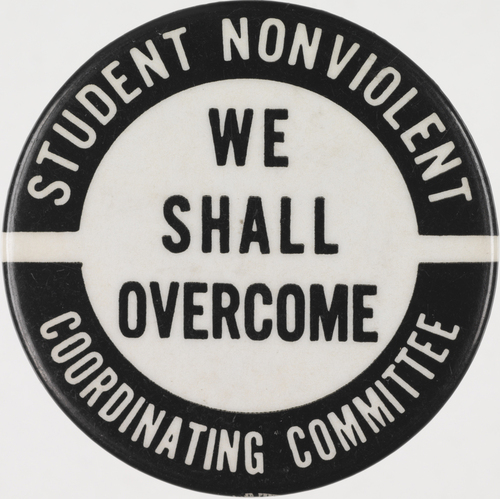
\includegraphics[max width=0.95\textwidth,
        max height=0.54000\textheight]{{Images/sncc}.jpg}
    \end{center}
    \end{column}
    \end{columns}
}
\end{frame}
\begin{frame}[t]{Round 3 --- Civil Rights Movements --- \mbox{Answer 7}}
\vspace{-0.5em}
\begin{block}{Question}
What is the commodity that Gandhi, in an act of civil disobedience, produced in violation of a monopoly granted by the British government?
\end{block}

\visible<2->{
    \begin{columns}[T,totalwidth=\linewidth]
    \begin{column}{0.32\linewidth}
    \begin{block}{Answer}
    Salt
    \end{block}
    \end{column}
    \begin{column}{0.65\linewidth}
    \begin{center}
    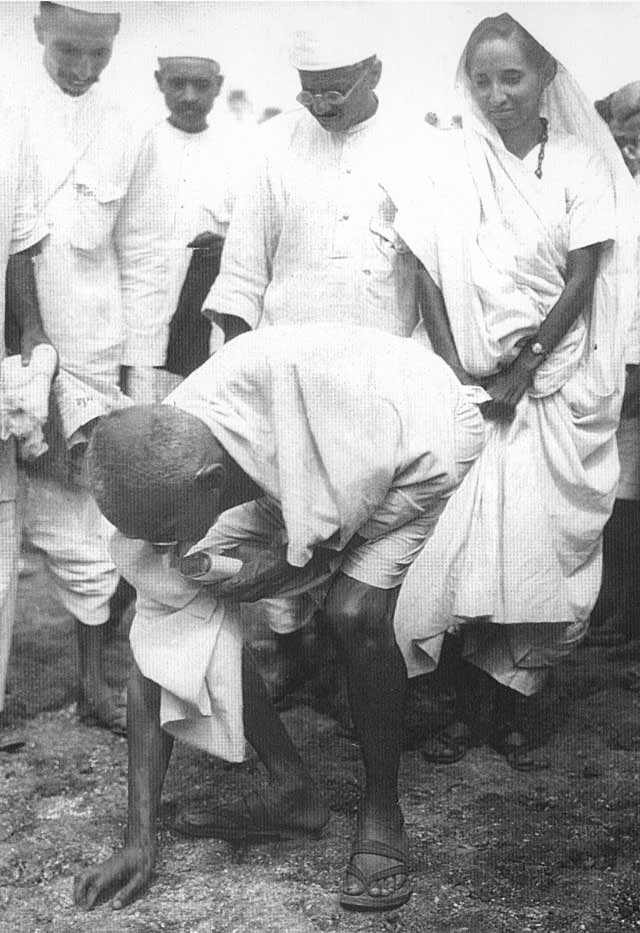
\includegraphics[max width=0.95\textwidth,
        max height=0.50000\textheight]{{Images/saltmarch}.jpg}
    \end{center}
    \end{column}
    \end{columns}
}
\end{frame}
\begin{frame}[t]{Round 3 --- Civil Rights Movements --- \mbox{Answer 8}}
\vspace{-0.5em}
\begin{block}{Question}
What is the name of the essay in which Martin Luther King argued to fellow clergy that they were wrong in saying that the time was not yet right for action on civil rights?
\end{block}

\visible<2->{
    \begin{columns}[T,totalwidth=\linewidth]
    \begin{column}{0.32\linewidth}
    \begin{block}{Answer}
    Letter from a Birmingham Jail
    \end{block}
    \end{column}
    \begin{column}{0.65\linewidth}
    \begin{center}
    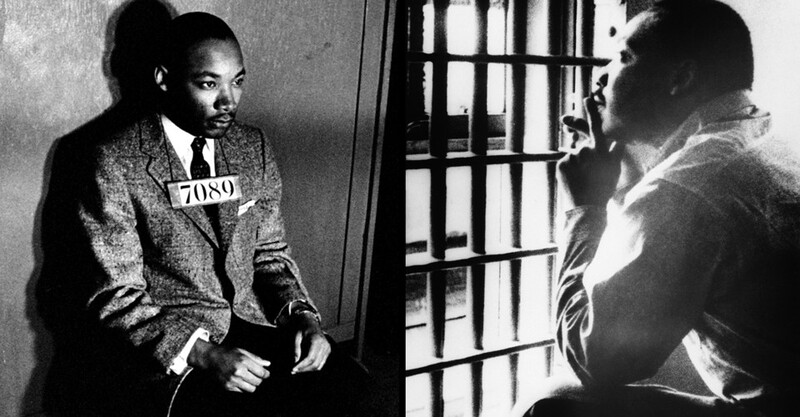
\includegraphics[max width=0.95\textwidth,
        max height=0.46000\textheight]{{Images/mlk}.jpg}
    \end{center}
    \end{column}
    \end{columns}
}
\end{frame}
\begin{frame}[t]{Round 3 --- Civil Rights Movements --- \mbox{Answer 9}}
\vspace{-0.5em}
\begin{block}{Question}
What is the name of the woman who was known as the ``The First Lady of the Struggle'' and who was the only African-American woman to be part of the U.S. delegation to the group that created of the United Nations charter?
\end{block}

\visible<2->{
    \begin{columns}[T,totalwidth=\linewidth]
    \begin{column}{0.32\linewidth}
    \begin{block}{Answer}
    Mary McLeod Bethune
    \end{block}
    \end{column}
    \begin{column}{0.65\linewidth}
    \begin{center}
    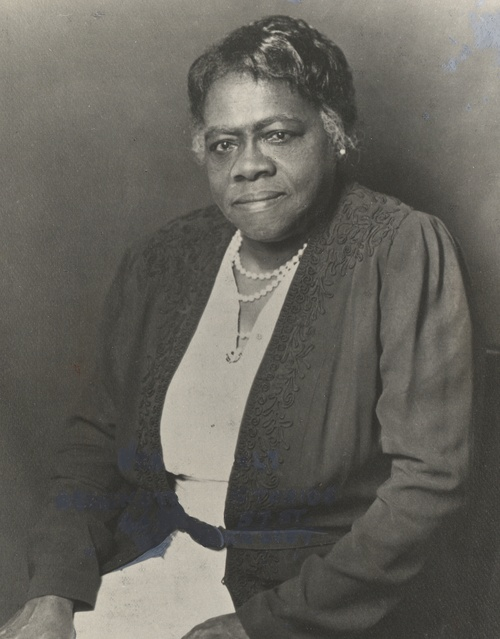
\includegraphics[max width=0.95\textwidth,
        max height=0.42000\textheight]{{Images/bethune}.jpg}
    \end{center}
    \end{column}
    \end{columns}
}
\end{frame}
\begin{frame}[t]{Round 3 --- Civil Rights Movements --- \mbox{Answer 10}}
\vspace{-0.5em}
\begin{block}{Question}
What is the name of the woman born in Mississippi in 1862 who became best known for her work as a crusading journalist  who exposed the prevalence and horror  of lynching?
\end{block}

\visible<2->{
    \begin{columns}[T,totalwidth=\linewidth]
    \begin{column}{0.32\linewidth}
    \begin{block}{Answer}
    Ida B. Wells
    \end{block}
    \end{column}
    \begin{column}{0.65\linewidth}
    \begin{center}
    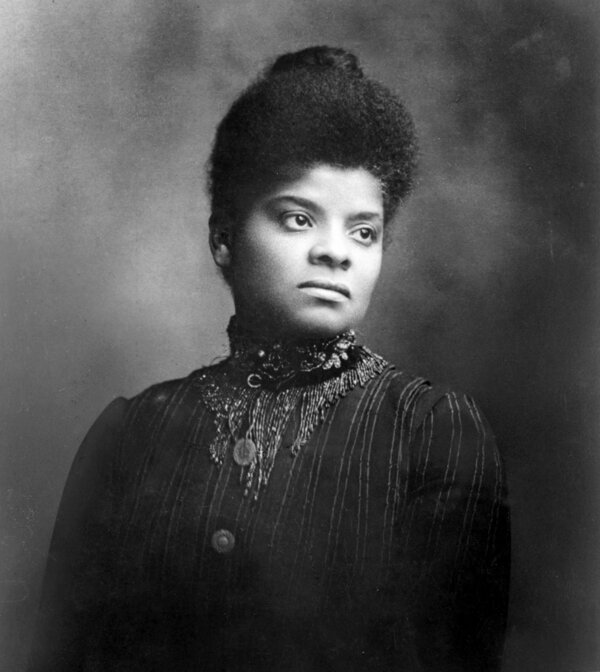
\includegraphics[max width=0.95\textwidth,
        max height=0.46000\textheight]{{Images/wells}.jpg}
    \end{center}
    \end{column}
    \end{columns}
}
\end{frame}
\def\thisSectionName{How Now Brown Cow?}
\section{Round 4}
\subsection*{Q1}
\begin{frame}[t]{Round 4 --- How Now Brown Cow? --- \mbox{Question 1}}
\vspace{-0.5em}
\begin{block}{Question}
Which dairy scientist was also a major contributor to the germ theory of diseases and helped create the vaccines for anthrax and rabies?
\end{block}
\end{frame}
\subsection*{Q2}
\begin{frame}[t]{Round 4 --- How Now Brown Cow? --- \mbox{Question 2}}
\vspace{-0.5em}
\begin{block}{Question}
In which U.S. state capital is the annual five-day World Dairy Expo held?
\end{block}
\end{frame}
\subsection*{Q3}
\begin{frame}[t]{Round 4 --- How Now Brown Cow? --- \mbox{Question 3}}
\vspace{-0.5em}
\begin{block}{Question}
\emph{Airag} and \emph{kurmis} are Mongolian fermented drinks made from the milk of what animal?
\end{block}
\end{frame}
\subsection*{Q4}
\begin{frame}[t]{Round 4 --- How Now Brown Cow? --- \mbox{Question 4}}
\vspace{-0.5em}
\begin{block}{Question}
According to a 2005 study by the British Cheese Board, what kind of British cheese can cause ``odd and vivid'' dreams when eaten shortly before going to sleep?
\end{block}
\end{frame}
\subsection*{Q5}
\begin{frame}[t]{Round 4 --- How Now Brown Cow? --- \mbox{Question 5}}
\vspace{-0.5em}
\begin{block}{Question}
What is the most popular ice cream flavor in the U.S.?
\end{block}
\end{frame}
\subsection*{Q6}
\begin{frame}[t]{Round 4 --- How Now Brown Cow? --- \mbox{Question 6}}
\vspace{-0.5em}
\begin{block}{Question}
Name either of the two kinds of bacteria primarily responsible for producing yogurt.
\end{block}
\end{frame}
\subsection*{Q7}
\begin{frame}[t]{Round 4 --- How Now Brown Cow? --- \mbox{Question 7}}
\vspace{-0.5em}
\begin{block}{Question}
What are the two primary dairy products required to make New York style cheesecake? (We need both.)
\end{block}
\end{frame}
\subsection*{Q8}
\begin{frame}[t]{Round 4 --- How Now Brown Cow? --- \mbox{Question 8}}
\vspace{-0.5em}
\begin{block}{Question}
According to the Purebred Dairy Cattle Association, there are seven major dairy cow breeds in the U.S\@. Name any one of them.
\end{block}
\end{frame}
\subsection*{Q9}
\begin{frame}[t]{Round 4 --- How Now Brown Cow? --- \mbox{Question 9}}
\vspace{-0.5em}
\begin{block}{Question}
Because milk is a mixture of two substances that cannot normally be mixed --- fat and water --- it is classified as what kind of substance?
\end{block}
\end{frame}
\subsection*{Q10}
\begin{frame}[t]{Round 4 --- How Now Brown Cow? --- \mbox{Question 10}}
\vspace{-0.5em}
\begin{block}{Question}
In milk, fat globules are surrounded by protein membranes that keep the fat suspended in the water. What is the name of the mechanical process by which these membranes are broken, allowing the milk's fats to clump together?
\end{block}
\end{frame}
\subsection{Answers}
\begin{frame}[t]{Round 4 --- How Now Brown Cow? --- \mbox{Answer 1}}
\vspace{-0.5em}
\begin{block}{Question}
Which dairy scientist was also a major contributor to the germ theory of diseases and helped create the vaccines for anthrax and rabies?
\end{block}

\visible<2->{
    \begin{columns}[T,totalwidth=\linewidth]
    \begin{column}{0.32\linewidth}
    \begin{block}{Answer}
    Louis Pasteur
    \end{block}
    \end{column}
    \begin{column}{0.65\linewidth}
    \begin{center}
    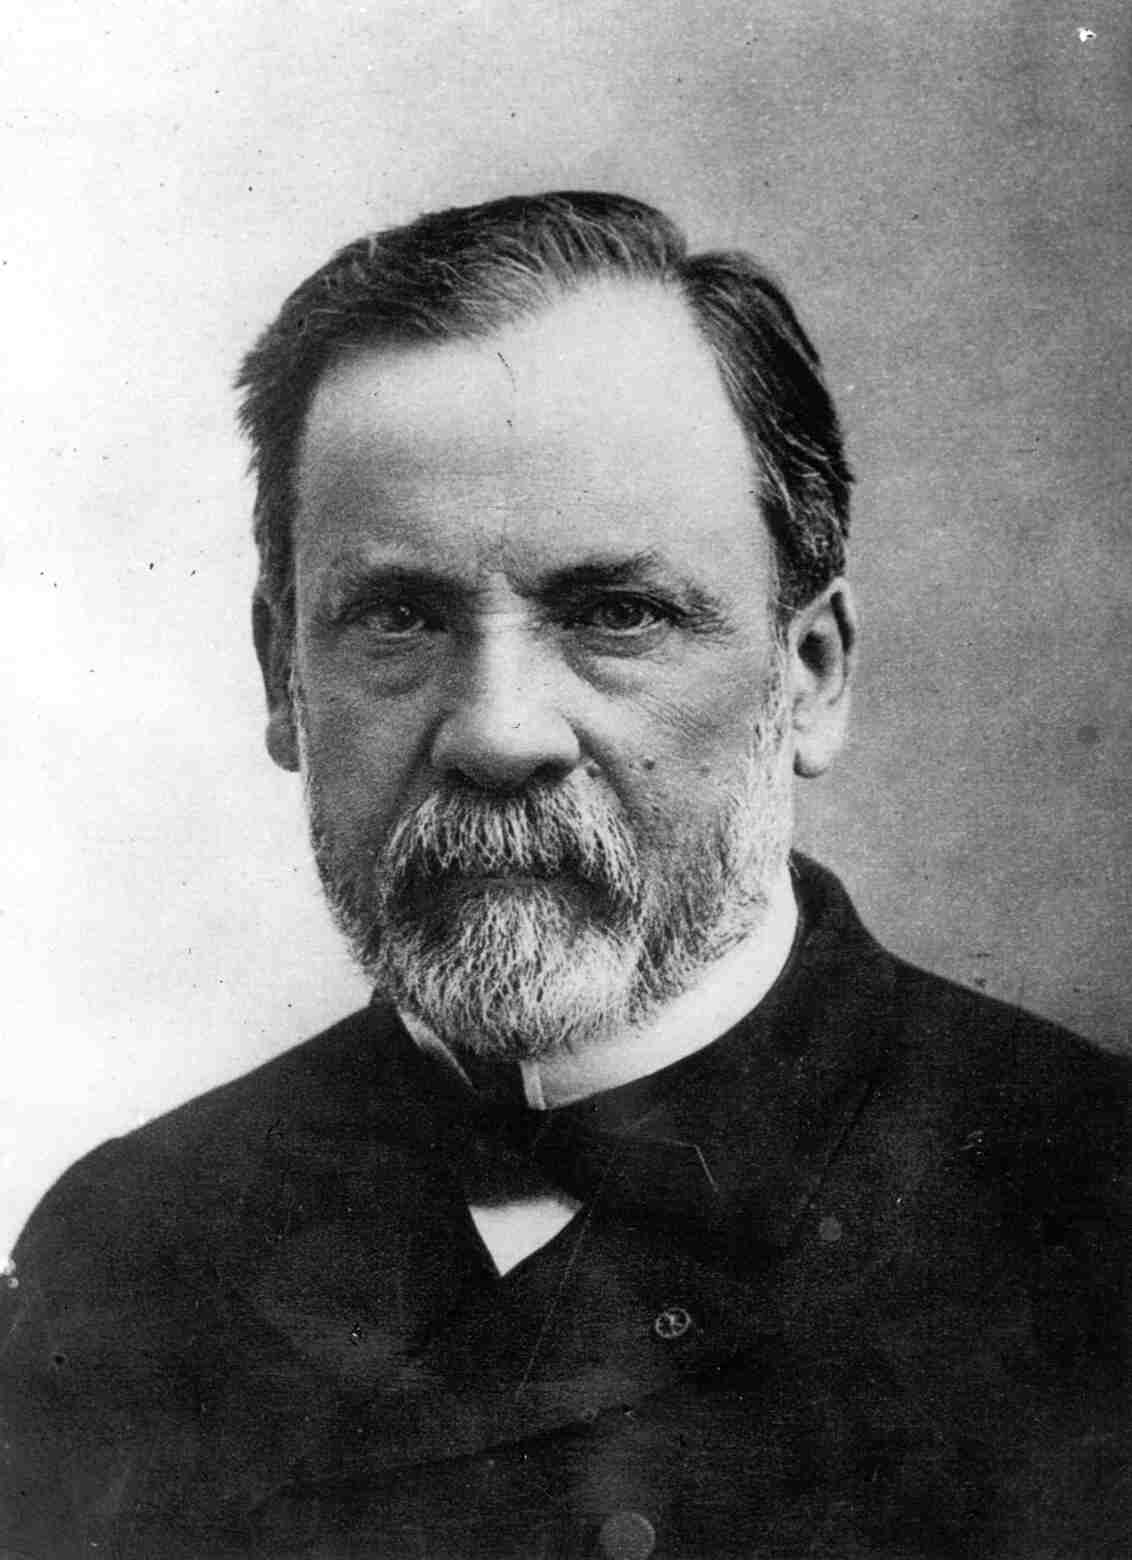
\includegraphics[max width=0.95\textwidth,
        max height=0.50000\textheight]{{Images/pasteur}.jpg}
    \end{center}
    \end{column}
    \end{columns}
}
\end{frame}
\begin{frame}[t]{Round 4 --- How Now Brown Cow? --- \mbox{Answer 2}}
\vspace{-0.5em}
\begin{block}{Question}
In which U.S. state capital is the annual five-day World Dairy Expo held?
\end{block}

\visible<2->{
    \begin{columns}[T,totalwidth=\linewidth]
    \begin{column}{0.32\linewidth}
    \begin{block}{Answer}
    Madison, WI
    \end{block}
    \end{column}
    \begin{column}{0.65\linewidth}
    \begin{center}
    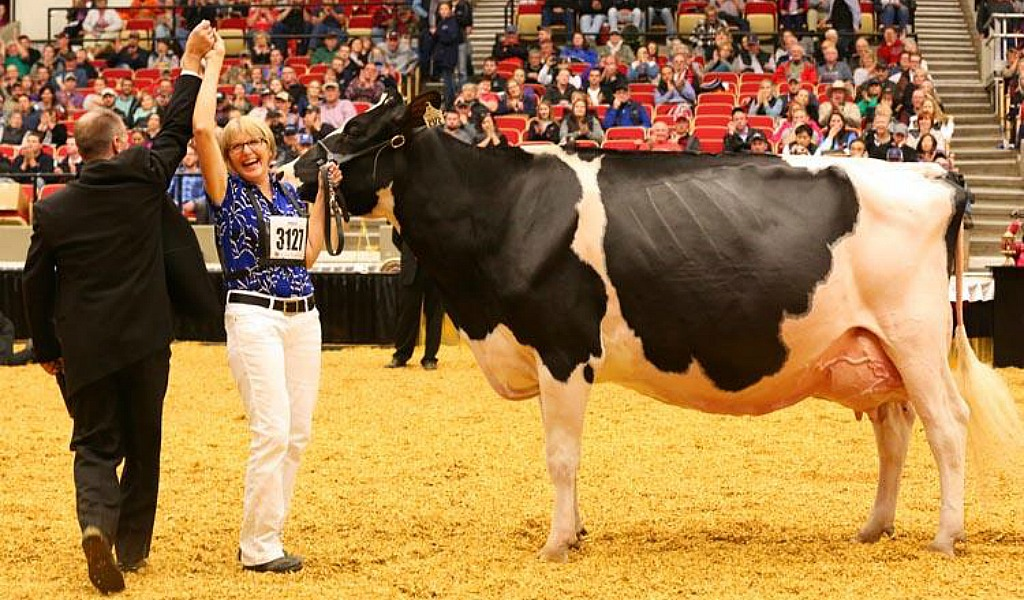
\includegraphics[max width=0.95\textwidth,
        max height=0.54000\textheight]{{Images/wde}.jpg}
    \end{center}
    \end{column}
    \end{columns}
}
\end{frame}
\begin{frame}[t]{Round 4 --- How Now Brown Cow? --- \mbox{Answer 3}}
\vspace{-0.5em}
\begin{block}{Question}
\emph{Airag} and \emph{kurmis} are Mongolian fermented drinks made from the milk of what animal?
\end{block}

\visible<2->{
    \begin{columns}[T,totalwidth=\linewidth]
    \begin{column}{0.32\linewidth}
    \begin{block}{Answer}
    Horses / mares
    \end{block}
    \end{column}
    \begin{column}{0.65\linewidth}
    \begin{center}
    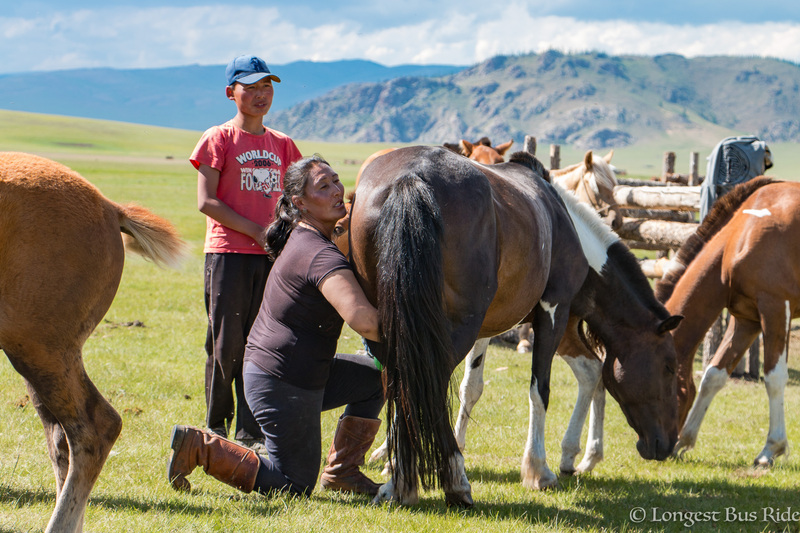
\includegraphics[max width=0.95\textwidth,
        max height=0.54000\textheight]{{Images/mongolianhorse}.jpg}
    \end{center}
    \end{column}
    \end{columns}
}
\end{frame}
\begin{frame}[t]{Round 4 --- How Now Brown Cow? --- \mbox{Answer 4}}
\vspace{-0.5em}
\begin{block}{Question}
According to a 2005 study by the British Cheese Board, what kind of British cheese can cause ``odd and vivid'' dreams when eaten shortly before going to sleep?
\end{block}

\visible<2->{
    \begin{columns}[T,totalwidth=\linewidth]
    \begin{column}{0.32\linewidth}
    \begin{block}{Answer}
    Stilton cheese
    \end{block}
    \end{column}
    \begin{column}{0.65\linewidth}
    \begin{center}
    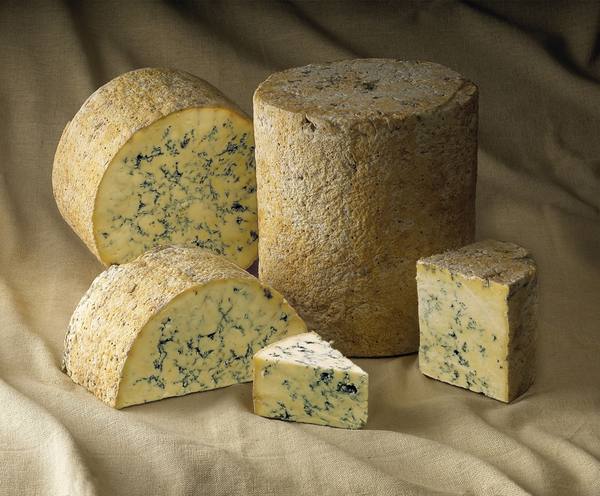
\includegraphics[max width=0.95\textwidth,
        max height=0.46000\textheight]{{Images/stilton}.jpg}
    \end{center}
    \end{column}
    \end{columns}
}
\end{frame}
\begin{frame}[t]{Round 4 --- How Now Brown Cow? --- \mbox{Answer 5}}
\vspace{-0.5em}
\begin{block}{Question}
What is the most popular ice cream flavor in the U.S.?
\end{block}

\visible<2->{
    \begin{columns}[T,totalwidth=\linewidth]
    \begin{column}{0.32\linewidth}
    \begin{block}{Answer}
    Vanilla
    \end{block}
    \end{column}
    \begin{column}{0.65\linewidth}
    \begin{center}
    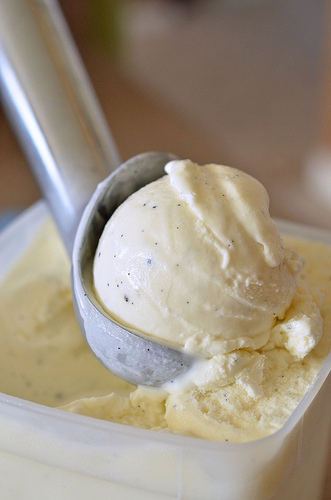
\includegraphics[max width=0.95\textwidth,
        max height=0.54000\textheight]{{Images/vanilla}.jpg}
    \end{center}
    \end{column}
    \end{columns}
}
\end{frame}
\begin{frame}[t]{Round 4 --- How Now Brown Cow? --- \mbox{Answer 6}}
\vspace{-0.5em}
\begin{block}{Question}
Name either of the two kinds of bacteria primarily responsible for producing yogurt.
\end{block}

\visible<2->{
    \begin{columns}[T,totalwidth=\linewidth]
    \begin{column}{0.32\linewidth}
    \begin{block}{Answer}
    \emph{Lactobacillus} and \emph{Streptococcus} (we only needed one)
    \end{block}
    \end{column}
    \begin{column}{0.65\linewidth}
    \begin{center}
    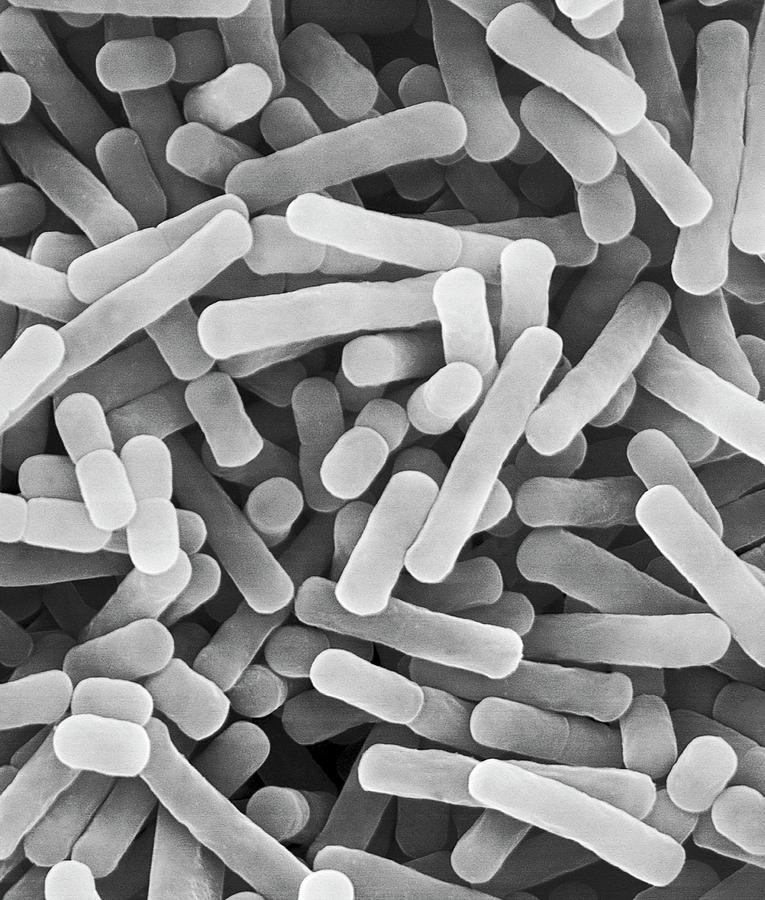
\includegraphics[max width=0.95\textwidth,
        max height=0.54000\textheight]{{Images/lacto}.jpg}
    \end{center}
    \end{column}
    \end{columns}
}
\end{frame}
\begin{frame}[t]{Round 4 --- How Now Brown Cow? --- \mbox{Answer 7}}
\vspace{-0.5em}
\begin{block}{Question}
What are the two primary dairy products required to make New York style cheesecake? (We need both.)
\end{block}

\visible<2->{
    \begin{columns}[T,totalwidth=\linewidth]
    \begin{column}{0.32\linewidth}
    \begin{block}{Answer}
    Cream cheese and sour cream
    \end{block}
    \end{column}
    \begin{column}{0.65\linewidth}
    \begin{center}
    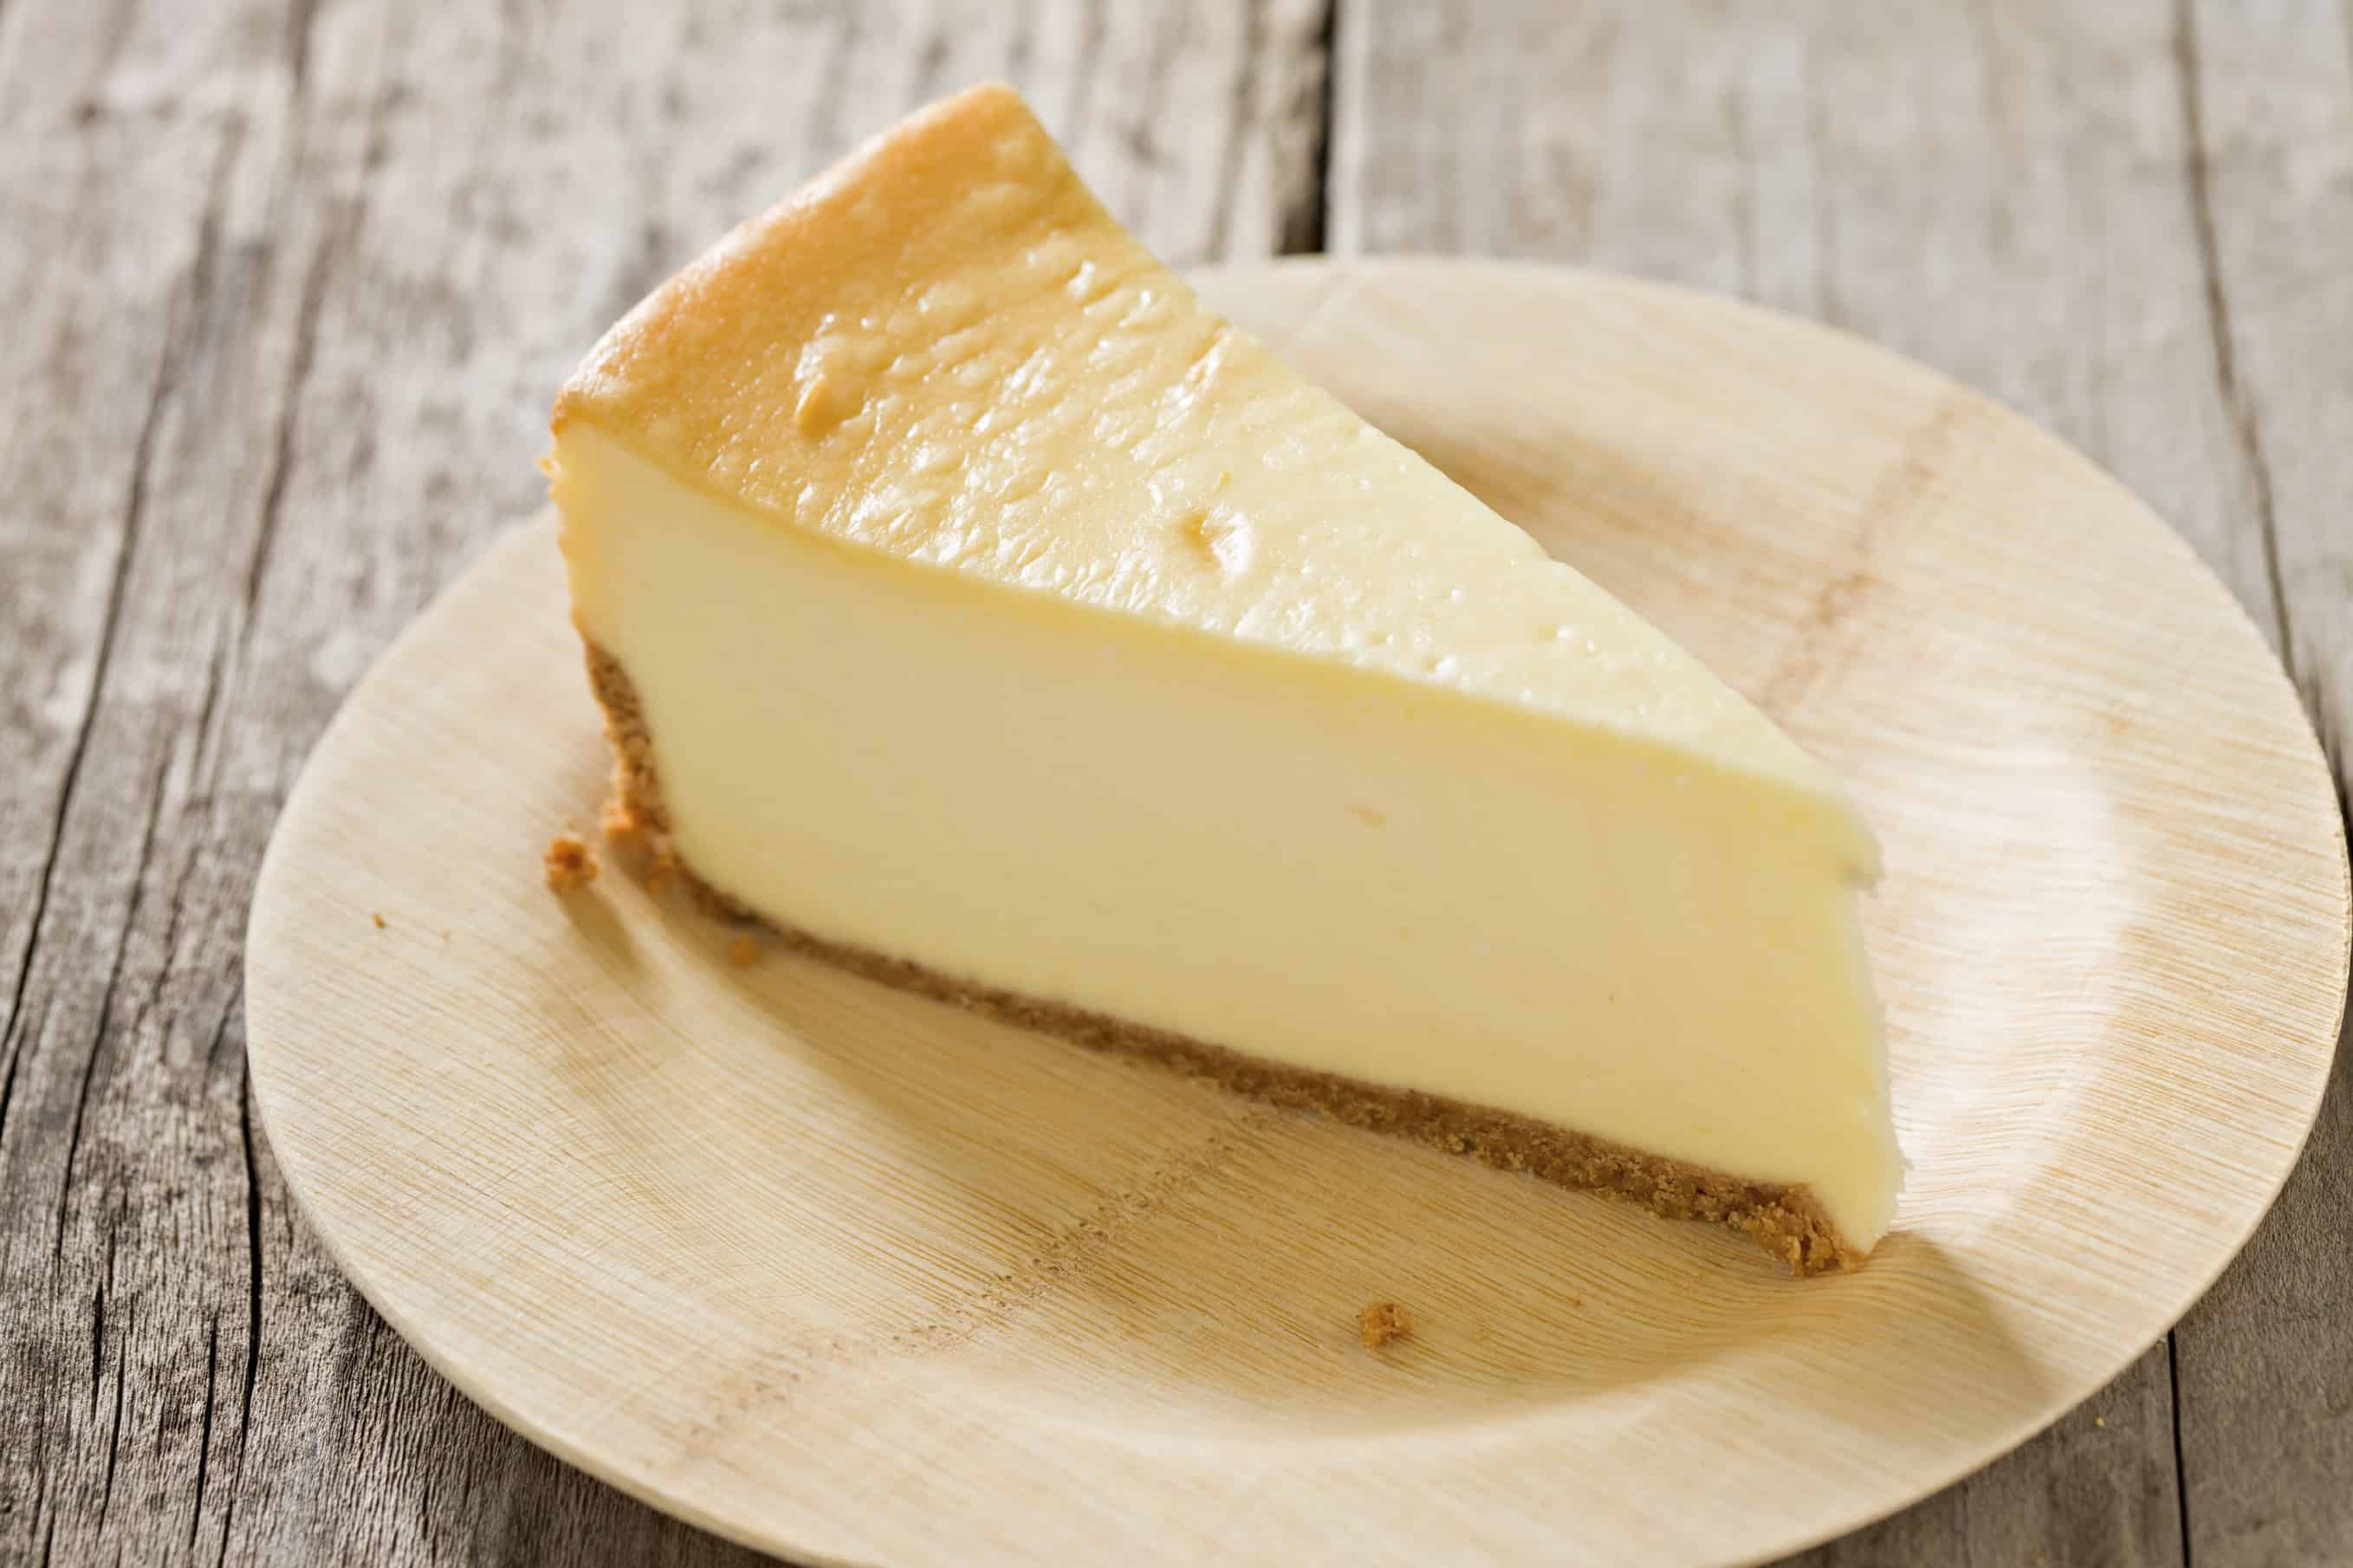
\includegraphics[max width=0.95\textwidth,
        max height=0.54000\textheight]{{Images/cheesecake}.jpg}
    \end{center}
    \end{column}
    \end{columns}
}
\end{frame}
\begin{frame}[t]{Round 4 --- How Now Brown Cow? --- \mbox{Answer 8}}
\vspace{-0.5em}
\begin{block}{Question}
According to the Purebred Dairy Cattle Association, there are seven major dairy cow breeds in the U.S\@. Name any one of them.
\end{block}

\visible<2->{
    \begin{columns}[T,totalwidth=\linewidth]
    \begin{column}{0.32\linewidth}
    \begin{block}{Answer}
    Any one of: Holstein, Brown Swiss, Guernsey, Ayrshire, Jersey, Red and White, and Milking Shorthorn
    \end{block}
    \end{column}
    \begin{column}{0.65\linewidth}
    \begin{center}
    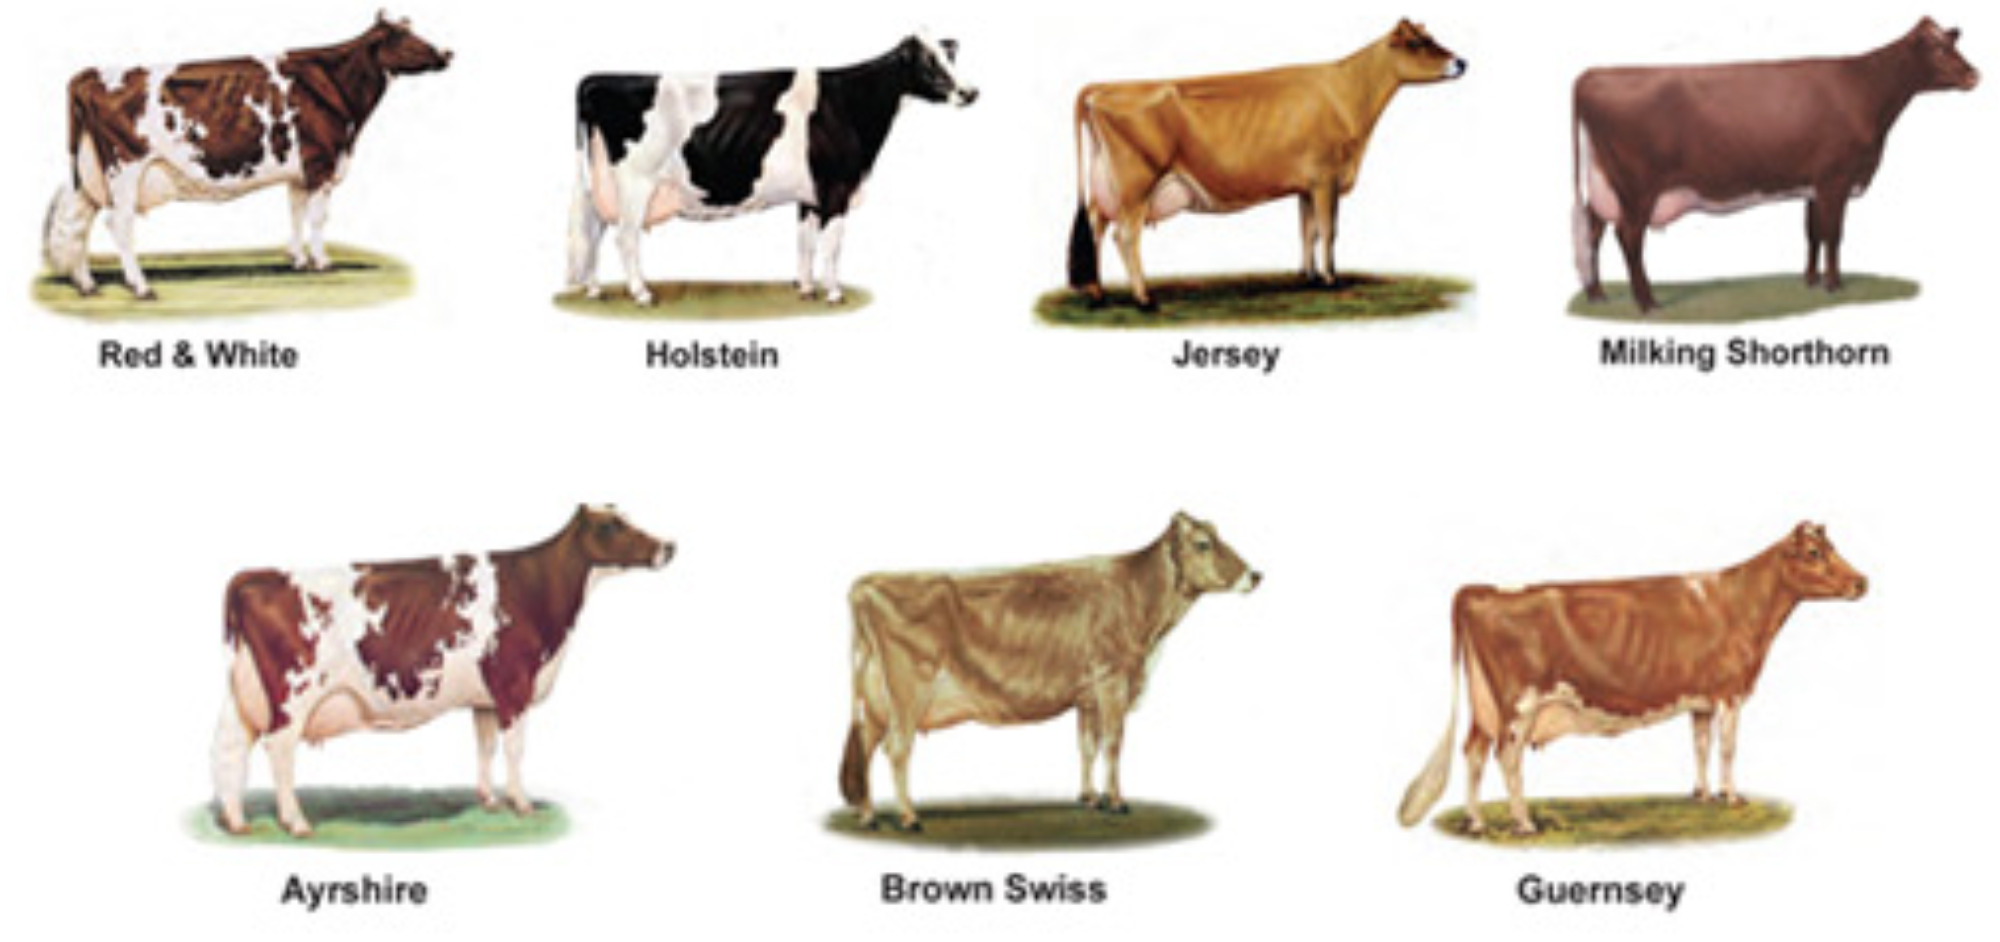
\includegraphics[max width=0.95\textwidth,
        max height=0.50000\textheight]{{Images/breeds}.jpg}
    \end{center}
    \end{column}
    \end{columns}
}
\end{frame}
\begin{frame}[t]{Round 4 --- How Now Brown Cow? --- \mbox{Answer 9}}
\vspace{-0.5em}
\begin{block}{Question}
Because milk is a mixture of two substances that cannot normally be mixed --- fat and water --- it is classified as what kind of substance?
\end{block}

\visible<2->{
    \begin{columns}[T,totalwidth=\linewidth]
    \begin{column}{0.32\linewidth}
    \begin{block}{Answer}
    An emulsion / colloid
    \end{block}
    \end{column}
    \begin{column}{0.65\linewidth}
    \begin{center}
    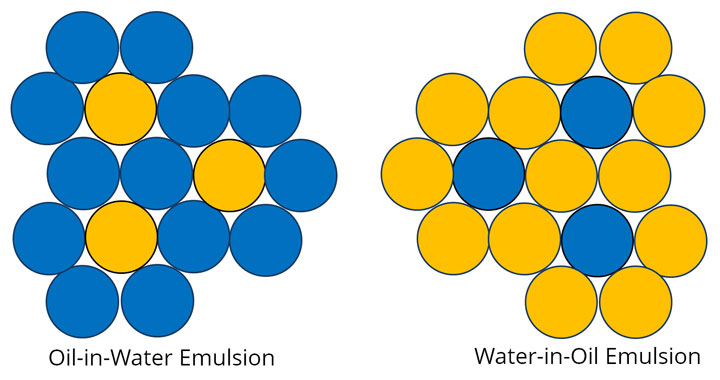
\includegraphics[max width=0.95\textwidth,
        max height=0.50000\textheight]{{Images/emulsion}.jpg}
    \end{center}
    \end{column}
    \end{columns}
}
\end{frame}
\begin{frame}[t]{Round 4 --- How Now Brown Cow? --- \mbox{Answer 10}}
\vspace{-0.5em}
\begin{block}{Question}
In milk, fat globules are surrounded by protein membranes that keep the fat suspended in the water. What is the name of the mechanical process by which these membranes are broken, allowing the milk's fats to clump together?
\end{block}

\visible<2->{
    \begin{columns}[T,totalwidth=\linewidth]
    \begin{column}{0.32\linewidth}
    \begin{block}{Answer}
    Churning (butter is ``de-emulsified'' milkfat)
    \end{block}
    \end{column}
    \begin{column}{0.65\linewidth}
    \begin{center}
    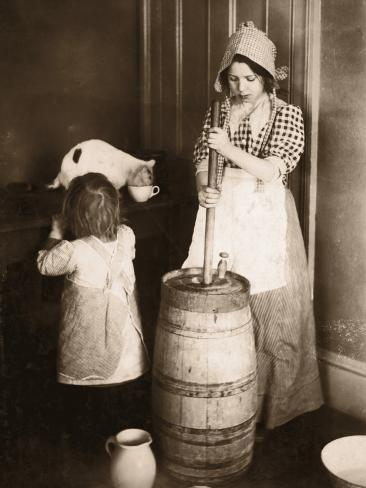
\includegraphics[max width=0.95\textwidth,
        max height=0.42000\textheight]{{Images/churn}.jpg}
    \end{center}
    \end{column}
    \end{columns}
}
\end{frame}
\def\thisSectionName{American Literature}
\section{Round 5}
\subsection*{Q1}
\begin{frame}[t]{Round 5 --- American Literature --- \mbox{Question 1}}
\vspace{-0.5em}
\begin{block}{Question}
What is the name of F. Scott Fitzgerald's first novel?
\end{block}
\end{frame}
\subsection*{Q2}
\begin{frame}[t]{Round 5 --- American Literature --- \mbox{Question 2}}
\vspace{-0.5em}
\begin{block}{Question}
Which poet wrote the line, ``For every atom belonging to me as good belongs to you''?
\end{block}
\end{frame}
\subsection*{Q3}
\begin{frame}[t]{Round 5 --- American Literature --- \mbox{Question 3}}
\vspace{-0.5em}
\begin{block}{Question}
Which 19\textsuperscript{th} century author of macabre poems and short stories was also an important literary theorist?
\end{block}
\end{frame}
\subsection*{Q4}
\begin{frame}[t]{Round 5 --- American Literature --- \mbox{Question 4}}
\vspace{-0.5em}
\begin{block}{Question}
What is the name of the fictional county that serves as the setting for many of many of William Faulkner's works?
\end{block}
\end{frame}
\subsection*{Q5}
\begin{frame}[t]{Round 5 --- American Literature --- \mbox{Question 5}}
\vspace{-0.5em}
\begin{block}{Question}
Who wrote the epic poem, ``Evangeline: A Tale of Acadie''?
\end{block}
\end{frame}
\subsection*{Q6}
\begin{frame}[t]{Round 5 --- American Literature --- \mbox{Question 6}}
\vspace{-0.5em}
\begin{block}{Question}
Who published a collection of poetry entitled \emph{Death and Taxes}?
\end{block}
\end{frame}
\subsection*{Q7}
\begin{frame}[t]{Round 5 --- American Literature --- \mbox{Question 7}}
\vspace{-0.5em}
\begin{block}{Question}
What is the name given to the group of authors that included Ralph Waldo Emerson, Henry David Thoreau and Margaret Fuller?
\end{block}
\end{frame}
\subsection*{Q8}
\begin{frame}[t]{Round 5 --- American Literature --- \mbox{Question 8}}
\vspace{-0.5em}
\begin{block}{Question}
What novel has a famous chapter entitled, ``Cetology''?
\end{block}
\end{frame}
\subsection*{Q9}
\begin{frame}[t]{Round 5 --- American Literature --- \mbox{Question 9}}
\vspace{-0.5em}
\begin{block}{Question}
What was the name of the Truman Capote work that Capote created by drawing on both journalistic and fiction-writing techniques?
\end{block}
\end{frame}
\subsection*{Q10}
\begin{frame}[t]{Round 5 --- American Literature --- \mbox{Question 10}}
\vspace{-0.5em}
\begin{block}{Question}
Who wrote \emph{The Age of Innocence}?
\end{block}
\end{frame}
\subsection{Answers}
\begin{frame}[t]{Round 5 --- American Literature --- \mbox{Answer 1}}
\vspace{-0.5em}
\begin{block}{Question}
What is the name of F. Scott Fitzgerald's first novel?
\end{block}

\visible<2->{
    \begin{columns}[T,totalwidth=\linewidth]
    \begin{column}{0.32\linewidth}
    \begin{block}{Answer}
    \emph{This Side of Paradise}
    \end{block}
    \end{column}
    \begin{column}{0.65\linewidth}
    \begin{center}
    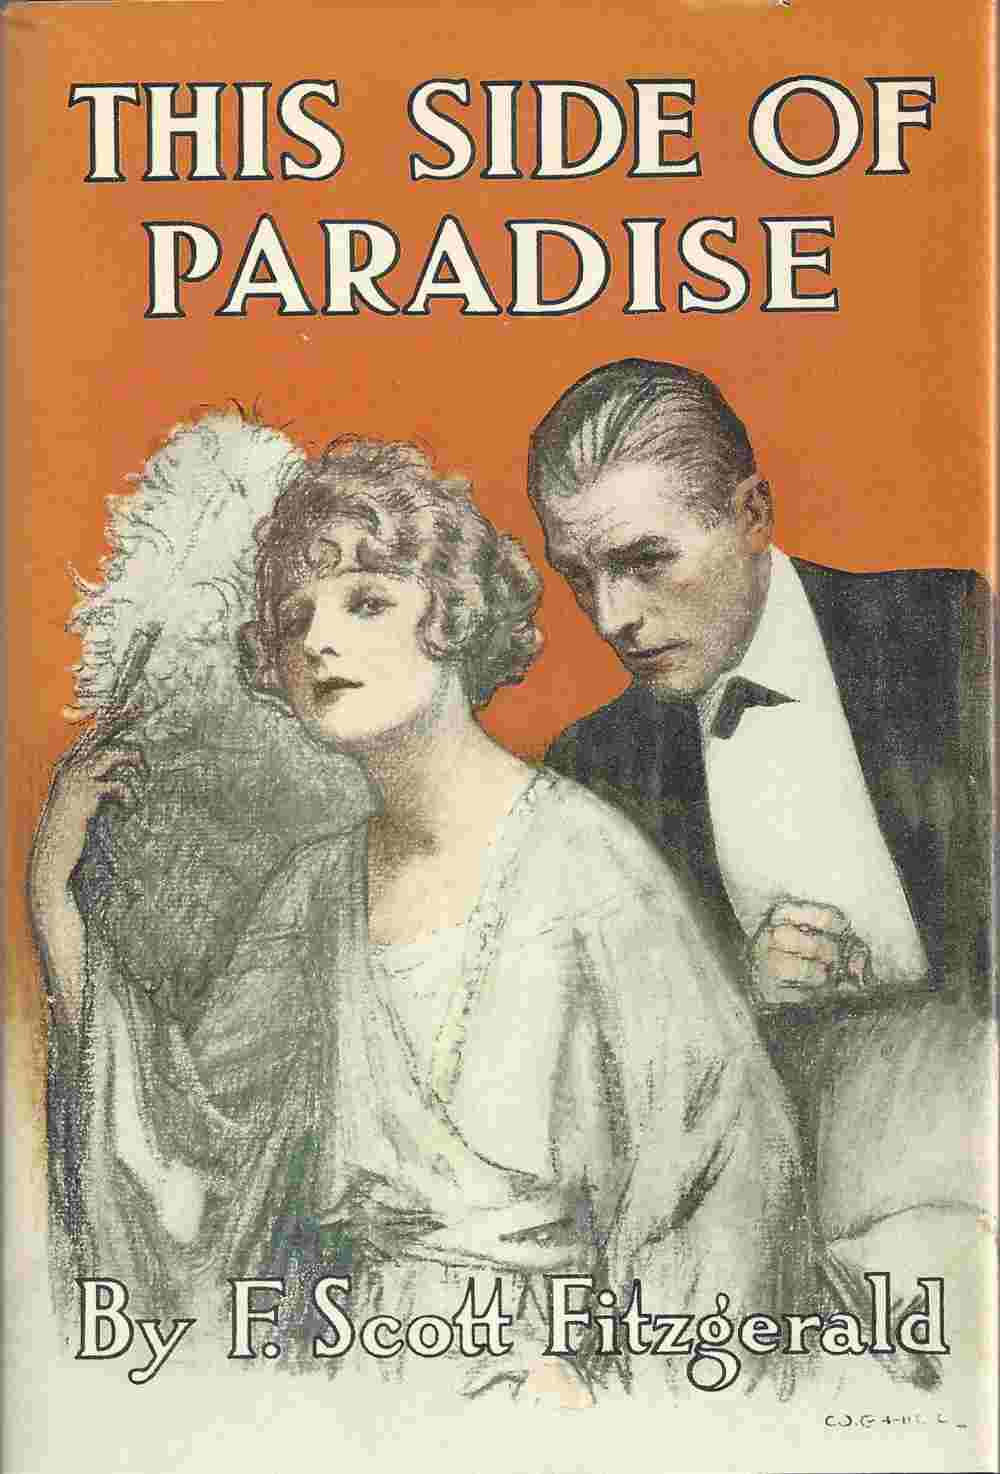
\includegraphics[max width=0.95\textwidth,
        max height=0.54000\textheight]{{Images/paradise}.jpg}
    \end{center}
    \end{column}
    \end{columns}
}
\end{frame}
\begin{frame}[t]{Round 5 --- American Literature --- \mbox{Answer 2}}
\vspace{-0.5em}
\begin{block}{Question}
Which poet wrote the line, ``For every atom belonging to me as good belongs to you''?
\end{block}

\visible<2->{
    \begin{columns}[T,totalwidth=\linewidth]
    \begin{column}{0.32\linewidth}
    \begin{block}{Answer}
    Walt Whitman
    \end{block}
    \end{column}
    \begin{column}{0.65\linewidth}
    \begin{center}
    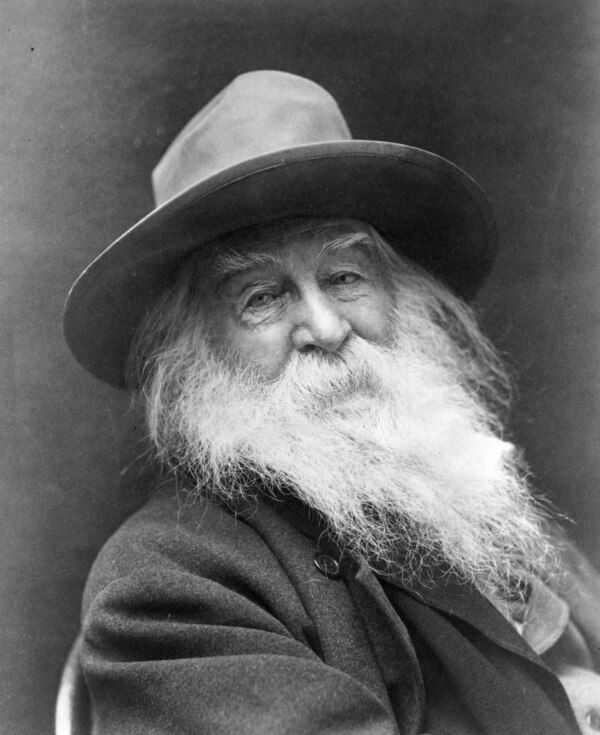
\includegraphics[max width=0.95\textwidth,
        max height=0.54000\textheight]{{Images/whitman}.jpg}
    \end{center}
    \end{column}
    \end{columns}
}
\end{frame}
\begin{frame}[t]{Round 5 --- American Literature --- \mbox{Answer 3}}
\vspace{-0.5em}
\begin{block}{Question}
Which 19\textsuperscript{th} century author of macabre poems and short stories was also an important literary theorist?
\end{block}

\visible<2->{
    \begin{columns}[T,totalwidth=\linewidth]
    \begin{column}{0.32\linewidth}
    \begin{block}{Answer}
    Edgar Allan Poe
    \end{block}
    \end{column}
    \begin{column}{0.65\linewidth}
    \begin{center}
    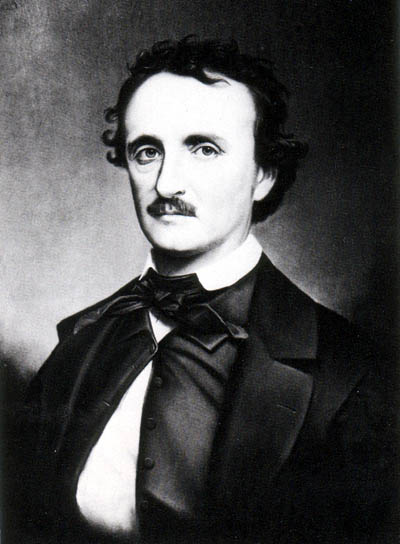
\includegraphics[max width=0.95\textwidth,
        max height=0.50000\textheight]{{Images/poe}.jpg}
    \end{center}
    \end{column}
    \end{columns}
}
\end{frame}
\begin{frame}[t]{Round 5 --- American Literature --- \mbox{Answer 4}}
\vspace{-0.5em}
\begin{block}{Question}
What is the name of the fictional county that serves as the setting for many of many of William Faulkner's works?
\end{block}

\visible<2->{
    \begin{columns}[T,totalwidth=\linewidth]
    \begin{column}{0.32\linewidth}
    \begin{block}{Answer}
    Yoknapatawpha County 
    \end{block}
    \end{column}
    \begin{column}{0.65\linewidth}
    \begin{center}
    \includegraphics[max width=0.95\textwidth,
        max height=0.50000\textheight]{{Images/yoknapatawpha}.jpg}
    \end{center}
    \end{column}
    \end{columns}
}
\end{frame}
\begin{frame}[t]{Round 5 --- American Literature --- \mbox{Answer 5}}
\vspace{-0.5em}
\begin{block}{Question}
Who wrote the epic poem, ``Evangeline: A Tale of Acadie''?
\end{block}

\visible<2->{
    \begin{columns}[T,totalwidth=\linewidth]
    \begin{column}{0.32\linewidth}
    \begin{block}{Answer}
    Henry Wadsworth Longfellow
    \end{block}
    \end{column}
    \begin{column}{0.65\linewidth}
    \begin{center}
    \includegraphics[max width=0.95\textwidth,
        max height=0.54000\textheight]{{Images/longfellow}.jpg}
    \end{center}
    \end{column}
    \end{columns}
}
\end{frame}
\begin{frame}[t]{Round 5 --- American Literature --- \mbox{Answer 6}}
\vspace{-0.5em}
\begin{block}{Question}
Who published a collection of poetry entitled \emph{Death and Taxes}?
\end{block}

\visible<2->{
    \begin{columns}[T,totalwidth=\linewidth]
    \begin{column}{0.32\linewidth}
    \begin{block}{Answer}
    Dorothy Parker
    \end{block}
    \end{column}
    \begin{column}{0.65\linewidth}
    \begin{center}
    \includegraphics[max width=0.95\textwidth,
        max height=0.54000\textheight]{{Images/dorothyparker}.jpg}
    \end{center}
    \end{column}
    \end{columns}
}
\end{frame}
\begin{frame}[t]{Round 5 --- American Literature --- \mbox{Answer 7}}
\vspace{-0.5em}
\begin{block}{Question}
What is the name given to the group of authors that included Ralph Waldo Emerson, Henry David Thoreau and Margaret Fuller?
\end{block}

\visible<2->{
    \begin{columns}[T,totalwidth=\linewidth]
    \begin{column}{0.32\linewidth}
    \begin{block}{Answer}
    The Transcendentalists
    \end{block}
    \end{column}
    \begin{column}{0.65\linewidth}
    \begin{center}
    \includegraphics[max width=0.95\textwidth,
        max height=0.50000\textheight]{{Images/transcend}.jpg}
    \end{center}
    \end{column}
    \end{columns}
}
\end{frame}
\begin{frame}[t]{Round 5 --- American Literature --- \mbox{Answer 8}}
\vspace{-0.5em}
\begin{block}{Question}
What novel has a famous chapter entitled, ``Cetology''?
\end{block}

\visible<2->{
    \begin{columns}[T,totalwidth=\linewidth]
    \begin{column}{0.32\linewidth}
    \begin{block}{Answer}
    \emph{Moby Dick}
    \end{block}
    \end{column}
    \begin{column}{0.65\linewidth}
    \begin{center}
    \includegraphics[max width=0.95\textwidth,
        max height=0.54000\textheight]{{Images/mobydick}.jpg}
    \end{center}
    \end{column}
    \end{columns}
}
\end{frame}
\begin{frame}[t]{Round 5 --- American Literature --- \mbox{Answer 9}}
\vspace{-0.5em}
\begin{block}{Question}
What was the name of the Truman Capote work that Capote created by drawing on both journalistic and fiction-writing techniques?
\end{block}

\visible<2->{
    \begin{columns}[T,totalwidth=\linewidth]
    \begin{column}{0.32\linewidth}
    \begin{block}{Answer}
    \emph{In Cold Blood}
    \end{block}
    \end{column}
    \begin{column}{0.65\linewidth}
    \begin{center}
    \includegraphics[max width=0.95\textwidth,
        max height=0.50000\textheight]{{Images/capote}.jpeg}
    \end{center}
    \end{column}
    \end{columns}
}
\end{frame}
\begin{frame}[t]{Round 5 --- American Literature --- \mbox{Answer 10}}
\vspace{-0.5em}
\begin{block}{Question}
Who wrote \emph{The Age of Innocence}?
\end{block}

\visible<2->{
    \begin{columns}[T,totalwidth=\linewidth]
    \begin{column}{0.32\linewidth}
    \begin{block}{Answer}
    Edith Wharton
    \end{block}
    \end{column}
    \begin{column}{0.65\linewidth}
    \begin{center}
    \includegraphics[max width=0.95\textwidth,
        max height=0.58000\textheight]{{Images/wharton}.jpg}
    \end{center}
    \end{column}
    \end{columns}
}
\end{frame}
\def\thisSectionName{Africa}
\section{Round 6}
\subsection*{Q1}
\begin{frame}[t]{Round 6 --- Africa --- \mbox{Question 1}}
\vspace{-0.5em}
\begin{block}{Question}
Which waterway connects the Mediterranean Sea and the Red Sea?
\end{block}
\end{frame}
\subsection*{Q2}
\begin{frame}[t]{Round 6 --- Africa --- \mbox{Question 2}}
\vspace{-0.5em}
\begin{block}{Question}
Which country's official currency is the rand?
\end{block}
\end{frame}
\subsection*{Q3}
\begin{frame}[t]{Round 6 --- Africa --- \mbox{Question 3}}
\vspace{-0.5em}
\begin{block}{Question}
In which country is the city of Tangier located?
\end{block}
\end{frame}
\subsection*{Q4}
\begin{frame}[t]{Round 6 --- Africa --- \mbox{Question 4}}
\vspace{-0.5em}
\begin{columns}[T,totalwidth=\linewidth]
\begin{column}{0.32\linewidth}
\begin{block}{Question}
What is the name of the Southern African desert that covers much of Botswana and is indicated by the red blob in the picture here? (The orange part surrounding it is the desert basin.)
\end{block}
\end{column}
\begin{column}{0.65\linewidth}
\begin{center}
\includegraphics[max width=0.95\textwidth,max height=0.7\textheight]{{Images/kalahari}.png}
\end{center}
\end{column}
\end{columns}
\end{frame}
\subsection*{Q5}
\begin{frame}[t]{Round 6 --- Africa --- \mbox{Question 5}}
\vspace{-0.5em}
\begin{block}{Question}
As specified in their constitution, what are the two official languages of Algeria?
\end{block}
\end{frame}
\subsection*{Q6}
\begin{frame}[t]{Round 6 --- Africa --- \mbox{Question 6}}
\vspace{-0.5em}
\begin{block}{Question}
Joseph Conrad's novel \emph{Heart of Darkness} tells the story of Charles Marlow's voyage along which real-life African river?
\end{block}
\end{frame}
\subsection*{Q7}
\begin{frame}[t]{Round 6 --- Africa --- \mbox{Question 7}}
\vspace{-0.5em}
\begin{block}{Question}
The territory formerly known as Rhodesia is now which country?
\end{block}
\end{frame}
\subsection*{Q8}
\begin{frame}[t]{Round 6 --- Africa --- \mbox{Question 8}}
\vspace{-0.5em}
\begin{columns}[T,totalwidth=\linewidth]
\begin{column}{0.32\linewidth}
\begin{block}{Question}
Which country's flag is pictured here?
\end{block}
\end{column}
\begin{column}{0.65\linewidth}
\begin{center}
\includegraphics[max width=0.95\textwidth,max height=0.7\textheight]{{Images/ghana}.png}
\end{center}
\end{column}
\end{columns}
\end{frame}
\subsection*{Q9}
\begin{frame}[t]{Round 6 --- Africa --- \mbox{Question 9}}
\vspace{-0.5em}
\begin{columns}[T,totalwidth=\linewidth]
\begin{column}{0.32\linewidth}
\begin{block}{Question}
What kind of African bovine is pictured here?
\end{block}
\end{column}
\begin{column}{0.65\linewidth}
\begin{center}
\includegraphics[max width=0.95\textwidth,max height=0.7\textheight]{{Images/gnu}.jpg}
\end{center}
\end{column}
\end{columns}
\end{frame}
\subsection*{Q10}
\begin{frame}[t]{Round 6 --- Africa --- \mbox{Question 10}}
\vspace{-0.5em}
\begin{block}{Question}
What is the capital of Kenya?
\end{block}
\end{frame}
\subsection{Answers}
\begin{frame}[t]{Round 6 --- Africa --- \mbox{Answer 1}}
\vspace{-0.5em}
\begin{block}{Question}
Which waterway connects the Mediterranean Sea and the Red Sea?
\end{block}

\visible<2->{
    \begin{columns}[T,totalwidth=\linewidth]
    \begin{column}{0.32\linewidth}
    \begin{block}{Answer}
    The Suez Canal
    \end{block}
    \end{column}
    \begin{column}{0.65\linewidth}
    \begin{center}
    \includegraphics[max width=0.95\textwidth,
        max height=0.54000\textheight]{{Images/suez}.jpeg}
    \end{center}
    \end{column}
    \end{columns}
}
\end{frame}
\begin{frame}[t]{Round 6 --- Africa --- \mbox{Answer 2}}
\vspace{-0.5em}
\begin{block}{Question}
Which country's official currency is the rand?
\end{block}

\visible<2->{
    \begin{columns}[T,totalwidth=\linewidth]
    \begin{column}{0.32\linewidth}
    \begin{block}{Answer}
    South Africa
    \end{block}
    \end{column}
    \begin{column}{0.65\linewidth}
    \begin{center}
    \includegraphics[max width=0.95\textwidth,
        max height=0.58000\textheight]{{Images/rand}.jpg}
    \end{center}
    \end{column}
    \end{columns}
}
\end{frame}
\begin{frame}[t]{Round 6 --- Africa --- \mbox{Answer 3}}
\vspace{-0.5em}
\begin{block}{Question}
In which country is the city of Tangier located?
\end{block}

\visible<2->{
    \begin{columns}[T,totalwidth=\linewidth]
    \begin{column}{0.32\linewidth}
    \begin{block}{Answer}
    Morocco
    \end{block}
    \end{column}
    \begin{column}{0.65\linewidth}
    \begin{center}
    \includegraphics[max width=0.95\textwidth,
        max height=0.58000\textheight]{{Images/tangier}.jpg}
    \end{center}
    \end{column}
    \end{columns}
}
\end{frame}
\begin{frame}[t]{Round 6 --- Africa --- \mbox{Answer 4}}
\vspace{-0.5em}
\begin{columns}[T,totalwidth=\linewidth]
\begin{column}{0.32\linewidth}
\begin{block}{Question}
What is the name of the Southern African desert that covers much of Botswana and is indicated by the red blob in the picture here? (The orange part surrounding it is the desert basin.)
\end{block}
\visible<2->{
    \begin{block}{Answer}
    The Kalahari Desert
    \end{block}
}
\end{column}
\begin{column}{0.65\linewidth}
\begin{center}
\includegraphics[max width=0.95\textwidth,max height=0.7\textheight]{{Images/kalahari}.png}
\end{center}
\end{column}
\end{columns}
\end{frame}
\begin{frame}[t]{Round 6 --- Africa --- \mbox{Answer 5}}
\vspace{-0.5em}
\begin{block}{Question}
As specified in their constitution, what are the two official languages of Algeria?
\end{block}

\visible<2->{
    \begin{columns}[T,totalwidth=\linewidth]
    \begin{column}{0.32\linewidth}
    \begin{block}{Answer}
    Arabic and Berber / Tamazight
    \end{block}
    \end{column}
    \begin{column}{0.65\linewidth}
    \begin{center}
    \includegraphics[max width=0.95\textwidth,
        max height=0.54000\textheight]{{Images/algeria}.jpg}
    \end{center}
    \end{column}
    \end{columns}
}
\end{frame}
\begin{frame}[t]{Round 6 --- Africa --- \mbox{Answer 6}}
\vspace{-0.5em}
\begin{block}{Question}
Joseph Conrad's novel \emph{Heart of Darkness} tells the story of Charles Marlow's voyage along which real-life African river?
\end{block}

\visible<2->{
    \begin{columns}[T,totalwidth=\linewidth]
    \begin{column}{0.32\linewidth}
    \begin{block}{Answer}
    The Congo River
    \end{block}
    \end{column}
    \begin{column}{0.65\linewidth}
    \begin{center}
    \includegraphics[max width=0.95\textwidth,
        max height=0.50000\textheight]{{Images/congo}.jpg}
    \end{center}
    \end{column}
    \end{columns}
}
\end{frame}
\begin{frame}[t]{Round 6 --- Africa --- \mbox{Answer 7}}
\vspace{-0.5em}
\begin{block}{Question}
The territory formerly known as Rhodesia is now which country?
\end{block}

\visible<2->{
    \begin{columns}[T,totalwidth=\linewidth]
    \begin{column}{0.32\linewidth}
    \begin{block}{Answer}
    Zimbabwe
    \end{block}
    \end{column}
    \begin{column}{0.65\linewidth}
    \begin{center}
    \includegraphics[max width=0.95\textwidth,
        max height=0.54000\textheight]{{Images/zimbabwe}.jpg}
    \end{center}
    \end{column}
    \end{columns}
}
\end{frame}
\begin{frame}[t]{Round 6 --- Africa --- \mbox{Answer 8}}
\vspace{-0.5em}
\begin{columns}[T,totalwidth=\linewidth]
\begin{column}{0.32\linewidth}
\begin{block}{Question}
Which country's flag is pictured here?
\end{block}
\visible<2->{
    \begin{block}{Answer}
    Ghana
    \end{block}
}
\end{column}
\begin{column}{0.65\linewidth}
\begin{center}
\includegraphics[max width=0.95\textwidth,max height=0.7\textheight]{{Images/ghana}.png}
\end{center}
\end{column}
\end{columns}
\end{frame}
\begin{frame}[t]{Round 6 --- Africa --- \mbox{Answer 9}}
\vspace{-0.5em}
\begin{columns}[T,totalwidth=\linewidth]
\begin{column}{0.32\linewidth}
\begin{block}{Question}
What kind of African bovine is pictured here?
\end{block}
\visible<2->{
    \begin{block}{Answer}
    Wildebeest / gnu
    \end{block}
}
\end{column}
\begin{column}{0.65\linewidth}
\begin{center}
\includegraphics[max width=0.95\textwidth,max height=0.7\textheight]{{Images/gnu}.jpg}
\end{center}
\end{column}
\end{columns}
\end{frame}
\begin{frame}[t]{Round 6 --- Africa --- \mbox{Answer 10}}
\vspace{-0.5em}
\begin{block}{Question}
What is the capital of Kenya?
\end{block}

\visible<2->{
    \begin{columns}[T,totalwidth=\linewidth]
    \begin{column}{0.32\linewidth}
    \begin{block}{Answer}
    Nairobi
    \end{block}
    \end{column}
    \begin{column}{0.65\linewidth}
    \begin{center}
    \includegraphics[max width=0.95\textwidth,
        max height=0.58000\textheight]{{Images/nairobi}.jpg}
    \end{center}
    \end{column}
    \end{columns}
}
\end{frame}
\def\thisSectionName{World War II}
\section{Round 7}
\subsection*{Q1}
\begin{frame}[t]{Round 7 --- World War II --- \mbox{Question 1}}
\vspace{-0.5em}
\begin{block}{Question}
What was the code name for the Battle of Normandy, which started with the Allied invasion of Normandy on D-Day?
\end{block}
\end{frame}
\subsection*{Q2}
\begin{frame}[t]{Round 7 --- World War II --- \mbox{Question 2}}
\vspace{-0.5em}
\begin{block}{Question}
Who was the German general known as the ``Desert Fox'' whose whose panzer tank divisions fought across North Africa?
\end{block}
\end{frame}
\subsection*{Q3}
\begin{frame}[t]{Round 7 --- World War II --- \mbox{Question 3}}
\vspace{-0.5em}
\begin{block}{Question}
Who was the Supreme Allied Commander in WWII\@?
\end{block}
\end{frame}
\subsection*{Q4}
\begin{frame}[t]{Round 7 --- World War II --- \mbox{Question 4}}
\vspace{-0.5em}
\begin{block}{Question}
Who was the American Army General who was known as ``Old Blood and Guts'' (and about whom his troops said, ``Sure, his guts, our blood'')?
\end{block}
\end{frame}
\subsection*{Q5}
\begin{frame}[t]{Round 7 --- World War II --- \mbox{Question 5}}
\vspace{-0.5em}
\begin{block}{Question}
What date did President Franklin Roosevelt describe as ``a date which will live in infamy''? (We need the month, day, and year.)
\end{block}
\end{frame}
\subsection*{Q6}
\begin{frame}[t]{Round 7 --- World War II --- \mbox{Question 6}}
\vspace{-0.5em}
\begin{block}{Question}
What was the collective name given by Allied troops in the South Pacific during World War II to the female English-speaking radio broadcasters of Japanese propaganda?
\end{block}
\end{frame}
\subsection*{Q7}
\begin{frame}[t]{Round 7 --- World War II --- \mbox{Question 7}}
\vspace{-0.5em}
\begin{block}{Question}
Who accepted the Japanese surrender on the battleship Missouri?
\end{block}
\end{frame}
\subsection*{Q8}
\begin{frame}[t]{Round 7 --- World War II --- \mbox{Question 8}}
\vspace{-0.5em}
\begin{block}{Question}
What was the Italian resistance group that fought the Fascists?
\end{block}
\end{frame}
\subsection*{Q9}
\begin{frame}[t]{Round 7 --- World War II --- \mbox{Question 9}}
\vspace{-0.5em}
\begin{block}{Question}
What is the name of the American soldier who received every military combat award for valor available from the U.S. Army, as well as French and Belgian awards for heroism, and who played himself in the movie \emph{To Hell and Back}?
\end{block}
\end{frame}
\subsection*{Q10}
\begin{frame}[t]{Round 7 --- World War II --- \mbox{Question 10}}
\vspace{-0.5em}
\begin{block}{Question}
Who was the WWII leader whose encouraging series of radio addresses to his countrymen included the following:  ``The destiny of the world is here\dots{}. Whatever happens, the flame of the French resistance must not be extinguished and will not be extinguished''?
\end{block}
\end{frame}
\subsection{Answers}
\begin{frame}[t]{Round 7 --- World War II --- \mbox{Answer 1}}
\vspace{-0.5em}
\begin{block}{Question}
What was the code name for the Battle of Normandy, which started with the Allied invasion of Normandy on D-Day?
\end{block}
\visible<2->{
    \begin{block}{Answer}
    Operation Overlord 
    \end{block}
}
\end{frame}
\begin{frame}[t]{Round 7 --- World War II --- \mbox{Answer 2}}
\vspace{-0.5em}
\begin{block}{Question}
Who was the German general known as the ``Desert Fox'' whose whose panzer tank divisions fought across North Africa?
\end{block}

\visible<2->{
    \begin{columns}[T,totalwidth=\linewidth]
    \begin{column}{0.32\linewidth}
    \begin{block}{Answer}
    Gen.\ Irwin Rommel
    \end{block}
    \end{column}
    \begin{column}{0.65\linewidth}
    \begin{center}
    \includegraphics[max width=0.95\textwidth,
        max height=0.50000\textheight]{{Images/rommel}.jpeg}
    \end{center}
    \end{column}
    \end{columns}
}
\end{frame}
\begin{frame}[t]{Round 7 --- World War II --- \mbox{Answer 3}}
\vspace{-0.5em}
\begin{block}{Question}
Who was the Supreme Allied Commander in WWII\@?
\end{block}

\visible<2->{
    \begin{columns}[T,totalwidth=\linewidth]
    \begin{column}{0.32\linewidth}
    \begin{block}{Answer}
    Gen.\ Dwight Eisenhower
    \end{block}
    \end{column}
    \begin{column}{0.65\linewidth}
    \begin{center}
    \includegraphics[max width=0.95\textwidth,
        max height=0.58000\textheight]{{Images/eisenhower}.jpg}
    \end{center}
    \end{column}
    \end{columns}
}
\end{frame}
\begin{frame}[t]{Round 7 --- World War II --- \mbox{Answer 4}}
\vspace{-0.5em}
\begin{block}{Question}
Who was the American Army General who was known as ``Old Blood and Guts'' (and about whom his troops said, ``Sure, his guts, our blood'')?
\end{block}

\visible<2->{
    \begin{columns}[T,totalwidth=\linewidth]
    \begin{column}{0.32\linewidth}
    \begin{block}{Answer}
    Gen.\ George S. Patton
    \end{block}
    \end{column}
    \begin{column}{0.65\linewidth}
    \begin{center}
    \includegraphics[max width=0.95\textwidth,
        max height=0.50000\textheight]{{Images/patton}.jpg}
    \end{center}
    \end{column}
    \end{columns}
}
\end{frame}
\begin{frame}[t]{Round 7 --- World War II --- \mbox{Answer 5}}
\vspace{-0.5em}
\begin{block}{Question}
What date did President Franklin Roosevelt describe as ``a date which will live in infamy''? (We need the month, day, and year.)
\end{block}

\visible<2->{
    \begin{columns}[T,totalwidth=\linewidth]
    \begin{column}{0.32\linewidth}
    \begin{block}{Answer}
    December 7, 1941 (the date of the attack on Pearl Harbor)
    \end{block}
    \end{column}
    \begin{column}{0.65\linewidth}
    \begin{center}
    \includegraphics[max width=0.95\textwidth,
        max height=0.50000\textheight]{{Images/pearlharbor}.jpg}
    \end{center}
    \end{column}
    \end{columns}
}
\end{frame}
\begin{frame}[t]{Round 7 --- World War II --- \mbox{Answer 6}}
\vspace{-0.5em}
\begin{block}{Question}
What was the collective name given by Allied troops in the South Pacific during World War II to the female English-speaking radio broadcasters of Japanese propaganda?
\end{block}

\visible<2->{
    \begin{columns}[T,totalwidth=\linewidth]
    \begin{column}{0.32\linewidth}
    \begin{block}{Answer}
    Tokyo Rose
    \end{block}
    \end{column}
    \begin{column}{0.65\linewidth}
    \begin{center}
    \includegraphics[max width=0.95\textwidth,
        max height=0.46000\textheight]{{Images/tokyorose}.jpg}
    \end{center}
    \end{column}
    \end{columns}
}
\end{frame}
\begin{frame}[t]{Round 7 --- World War II --- \mbox{Answer 7}}
\vspace{-0.5em}
\begin{block}{Question}
Who accepted the Japanese surrender on the battleship Missouri?
\end{block}

\visible<2->{
    \begin{columns}[T,totalwidth=\linewidth]
    \begin{column}{0.32\linewidth}
    \begin{block}{Answer}
    Gen. Douglas MacArthur
    \end{block}
    \end{column}
    \begin{column}{0.65\linewidth}
    \begin{center}
    \includegraphics[max width=0.95\textwidth,
        max height=0.54000\textheight]{{Images/macarthur}.jpg}
    \end{center}
    \end{column}
    \end{columns}
}
\end{frame}
\begin{frame}[t]{Round 7 --- World War II --- \mbox{Answer 8}}
\vspace{-0.5em}
\begin{block}{Question}
What was the Italian resistance group that fought the Fascists?
\end{block}

\visible<2->{
    \begin{columns}[T,totalwidth=\linewidth]
    \begin{column}{0.32\linewidth}
    \begin{block}{Answer}
    The partisans / I partigiani
    \end{block}
    \end{column}
    \begin{column}{0.65\linewidth}
    \begin{center}
    \includegraphics[max width=0.95\textwidth,
        max height=0.54000\textheight]{{Images/partisans}.jpeg}
    \end{center}
    \end{column}
    \end{columns}
}
\end{frame}
\begin{frame}[t]{Round 7 --- World War II --- \mbox{Answer 9}}
\vspace{-0.5em}
\begin{block}{Question}
What is the name of the American soldier who received every military combat award for valor available from the U.S. Army, as well as French and Belgian awards for heroism, and who played himself in the movie \emph{To Hell and Back}?
\end{block}

\visible<2->{
    \begin{columns}[T,totalwidth=\linewidth]
    \begin{column}{0.32\linewidth}
    \begin{block}{Answer}
    Audie Murphy
    \end{block}
    \end{column}
    \begin{column}{0.65\linewidth}
    \begin{center}
    \includegraphics[max width=0.95\textwidth,
        max height=0.42000\textheight]{{Images/murphy}.jpeg}
    \end{center}
    \end{column}
    \end{columns}
}
\end{frame}
\begin{frame}[t]{Round 7 --- World War II --- \mbox{Answer 10}}
\vspace{-0.5em}
\begin{block}{Question}
Who was the WWII leader whose encouraging series of radio addresses to his countrymen included the following:  ``The destiny of the world is here\dots{}. Whatever happens, the flame of the French resistance must not be extinguished and will not be extinguished''?
\end{block}

\visible<2->{
    \begin{columns}[T,totalwidth=\linewidth]
    \begin{column}{0.32\linewidth}
    \begin{block}{Answer}
    Gen. Charles DeGaulle
    \end{block}
    \end{column}
    \begin{column}{0.65\linewidth}
    \begin{center}
    \includegraphics[max width=0.95\textwidth,
        max height=0.38000\textheight]{{Images/degaulle}.jpg}
    \end{center}
    \end{column}
    \end{columns}
}
\end{frame}
\def\thisSectionName{Competitions}
\section{Round 8}
\subsection*{Q1}
\begin{frame}[t]{Round 8 --- Competitions --- \mbox{Question 1}}
\vspace{-0.5em}
\begin{block}{Question}
Which MLB team won the 1986 World Series?
\end{block}
\end{frame}
\subsection*{Q2}
\begin{frame}[t]{Round 8 --- Competitions --- \mbox{Question 2}}
\vspace{-0.5em}
\begin{block}{Question}
In 1824, who was elected president by the House of Representatives after no presidential candidate received a majority of the Electoral College vote?
\end{block}
\end{frame}
\subsection*{Q3}
\begin{frame}[t]{Round 8 --- Competitions --- \mbox{Question 3}}
\vspace{-0.5em}
\begin{block}{Question}
Which boxing match currently holds the record for the highest-grossing pay-per-view boxing match? 
\end{block}
\end{frame}
\subsection*{Q4}
\begin{frame}[t]{Round 8 --- Competitions --- \mbox{Question 4}}
\vspace{-0.5em}
\begin{block}{Question}
How many Oscars has Leonardo DiCaprio won?
\end{block}
\end{frame}
\subsection*{Q5}
\begin{frame}[t]{Round 8 --- Competitions --- \mbox{Question 5}}
\vspace{-0.5em}
\begin{block}{Question}
Which contestant has cumulatively won the most money on \emph{Jeopardy!}?
\end{block}
\end{frame}
\subsection*{Q6}
\begin{frame}[t]{Round 8 --- Competitions --- \mbox{Question 6}}
\vspace{-0.5em}
\begin{block}{Question}
The Miracle on Ice was the 1980 Olympics ice hockey game in which the U.S. beat the Soviets, but that game was only a semifinal game. Which country's team did the U.S. defeat in the 1980 Olympics championship ice hockey game to win the gold medal?
\end{block}
\end{frame}
\subsection*{Q7}
\begin{frame}[t]{Round 8 --- Competitions --- \mbox{Question 7}}
\vspace{-0.5em}
\begin{block}{Question}
Who won the very first season of \emph{American Idol}\,?
\end{block}
\end{frame}
\subsection*{Q8}
\begin{frame}[t]{Round 8 --- Competitions --- \mbox{Question 8}}
\vspace{-0.5em}
\begin{block}{Question}
In what category of ``sports'' is it allowed, and even expected, that players will take stimulants such as Ritalin and Adderall before playing?
\end{block}
\end{frame}
\subsection*{Q9}
\begin{frame}[t]{Round 8 --- Competitions --- \mbox{Question 9}}
\vspace{-0.5em}
\begin{block}{Question}
Which Scrabble player is the only player to have won the World Scrabble Championship more than once? (He's won five times.)
\end{block}
\end{frame}
\subsection*{Q10}
\begin{frame}[t]{Round 8 --- Competitions --- \mbox{Question 10}}
\vspace{-0.5em}
\begin{block}{Question}
Which city has hosted the Summer Olympics the most times?
\end{block}
\end{frame}
\subsection{Answers}
\begin{frame}[t]{Round 8 --- Competitions --- \mbox{Answer 1}}
\vspace{-0.5em}
\begin{block}{Question}
Which MLB team won the 1986 World Series?
\end{block}

\visible<2->{
    \begin{columns}[T,totalwidth=\linewidth]
    \begin{column}{0.32\linewidth}
    \begin{block}{Answer}
    The Mets
    \end{block}
    \end{column}
    \begin{column}{0.65\linewidth}
    \begin{center}
    \includegraphics[max width=0.95\textwidth,
        max height=0.58000\textheight]{{Images/mets}.jpg}
    \end{center}
    \end{column}
    \end{columns}
}
\end{frame}
\begin{frame}[t]{Round 8 --- Competitions --- \mbox{Answer 2}}
\vspace{-0.5em}
\begin{block}{Question}
In 1824, who was elected president by the House of Representatives after no presidential candidate received a majority of the Electoral College vote?
\end{block}

\visible<2->{
    \begin{columns}[T,totalwidth=\linewidth]
    \begin{column}{0.32\linewidth}
    \begin{block}{Answer}
    John Quincy Adams
    \end{block}
    \end{column}
    \begin{column}{0.65\linewidth}
    \begin{center}
    \includegraphics[max width=0.95\textwidth,
        max height=0.50000\textheight]{{Images/jqa}.jpg}
    \end{center}
    \end{column}
    \end{columns}
}
\end{frame}
\begin{frame}[t]{Round 8 --- Competitions --- \mbox{Answer 3}}
\vspace{-0.5em}
\begin{block}{Question}
Which boxing match currently holds the record for the highest-grossing pay-per-view boxing match? 
\end{block}

\visible<2->{
    \begin{columns}[T,totalwidth=\linewidth]
    \begin{column}{0.32\linewidth}
    \begin{block}{Answer}
    Mayweather vs.\ Pacquiao (approximately \$410M)
    \end{block}
    \end{column}
    \begin{column}{0.65\linewidth}
    \begin{center}
    \includegraphics[max width=0.95\textwidth,
        max height=0.54000\textheight]{{Images/pacquiao}.jpg}
    \end{center}
    \end{column}
    \end{columns}
}
\end{frame}
\begin{frame}[t]{Round 8 --- Competitions --- \mbox{Answer 4}}
\vspace{-0.5em}
\begin{block}{Question}
How many Oscars has Leonardo DiCaprio won?
\end{block}

\visible<2->{
    \begin{columns}[T,totalwidth=\linewidth]
    \begin{column}{0.32\linewidth}
    \begin{block}{Answer}
    One (for \emph{The Revenant})
    \end{block}
    \end{column}
    \begin{column}{0.65\linewidth}
    \begin{center}
    \includegraphics[max width=0.95\textwidth,
        max height=0.58000\textheight]{{Images/revenant}.jpg}
    \end{center}
    \end{column}
    \end{columns}
}
\end{frame}
\begin{frame}[t]{Round 8 --- Competitions --- \mbox{Answer 5}}
\vspace{-0.5em}
\begin{block}{Question}
Which contestant has cumulatively won the most money on \emph{Jeopardy!}?
\end{block}

\visible<2->{
    \begin{columns}[T,totalwidth=\linewidth]
    \begin{column}{0.32\linewidth}
    \begin{block}{Answer}
    Brad Rutter (\$4,688,436 cumulatively over regular games and several \emph{Jeopardy!} tournaments)
    \end{block}
    \end{column}
    \begin{column}{0.65\linewidth}
    \begin{center}
    \includegraphics[max width=0.95\textwidth,
        max height=0.54000\textheight]{{Images/rutter}.jpg}
    \end{center}
    \end{column}
    \end{columns}
}
\end{frame}
\begin{frame}[t]{Round 8 --- Competitions --- \mbox{Answer 6}}
\vspace{-0.5em}
\begin{block}{Question}
The Miracle on Ice was the 1980 Olympics ice hockey game in which the U.S. beat the Soviets, but that game was only a semifinal game. Which country's team did the U.S. defeat in the 1980 Olympics championship ice hockey game to win the gold medal?
\end{block}

\visible<2->{
    \begin{columns}[T,totalwidth=\linewidth]
    \begin{column}{0.32\linewidth}
    \begin{block}{Answer}
    Finland
    \end{block}
    \end{column}
    \begin{column}{0.65\linewidth}
    \begin{center}
    \includegraphics[max width=0.95\textwidth,
        max height=0.42000\textheight]{{Images/miracle}.jpg}
    \end{center}
    \end{column}
    \end{columns}
}
\end{frame}
\begin{frame}[t]{Round 8 --- Competitions --- \mbox{Answer 7}}
\vspace{-0.5em}
\begin{block}{Question}
Who won the very first season of \emph{American Idol}\,?
\end{block}

\visible<2->{
    \begin{columns}[T,totalwidth=\linewidth]
    \begin{column}{0.32\linewidth}
    \begin{block}{Answer}
    Kelly Clarkson
    \end{block}
    \end{column}
    \begin{column}{0.65\linewidth}
    \begin{center}
    \includegraphics[max width=0.95\textwidth,
        max height=0.54000\textheight]{{Images/clarkson}.jpg}
    \end{center}
    \end{column}
    \end{columns}
}
\end{frame}
\begin{frame}[t]{Round 8 --- Competitions --- \mbox{Answer 8}}
\vspace{-0.5em}
\begin{block}{Question}
In what category of ``sports'' is it allowed, and even expected, that players will take stimulants such as Ritalin and Adderall before playing?
\end{block}

\visible<2->{
    \begin{columns}[T,totalwidth=\linewidth]
    \begin{column}{0.32\linewidth}
    \begin{block}{Answer}
    Esports
    \end{block}
    \end{column}
    \begin{column}{0.65\linewidth}
    \begin{center}
    \includegraphics[max width=0.95\textwidth,
        max height=0.50000\textheight]{{Images/esports}.jpg}
    \end{center}
    \end{column}
    \end{columns}
}
\end{frame}
\begin{frame}[t]{Round 8 --- Competitions --- \mbox{Answer 9}}
\vspace{-0.5em}
\begin{block}{Question}
Which Scrabble player is the only player to have won the World Scrabble Championship more than once? (He's won five times.)
\end{block}

\visible<2->{
    \begin{columns}[T,totalwidth=\linewidth]
    \begin{column}{0.32\linewidth}
    \begin{block}{Answer}
    Nigel Richards
    \end{block}
    \end{column}
    \begin{column}{0.65\linewidth}
    \begin{center}
    \includegraphics[max width=0.95\textwidth,
        max height=0.50000\textheight]{{Images/richards}.jpeg}
    \end{center}
    \end{column}
    \end{columns}
}
\end{frame}
\begin{frame}[t]{Round 8 --- Competitions --- \mbox{Answer 10}}
\vspace{-0.5em}
\begin{block}{Question}
Which city has hosted the Summer Olympics the most times?
\end{block}

\visible<2->{
    \begin{columns}[T,totalwidth=\linewidth]
    \begin{column}{0.32\linewidth}
    \begin{block}{Answer}
    London (three times: in 1908, 1948, and 2012)
    \end{block}
    \end{column}
    \begin{column}{0.65\linewidth}
    \begin{center}
    \includegraphics[max width=0.95\textwidth,
        max height=0.54000\textheight]{{Images/london}.jpg}
    \end{center}
    \end{column}
    \end{columns}
}
\end{frame}
\def\thisSectionName{Name the Film from the Cast}
\section{Round 9}
\subsection*{Q1}
\begin{frame}[t]{Round 9 --- Name the Film from the Cast --- \mbox{Question 1}}
\vspace{-0.5em}
\begin{block}{Question}
Alan Ladd, Veronica Lake, Robert Preston
\end{block}
\end{frame}
\subsection*{Q2}
\begin{frame}[t]{Round 9 --- Name the Film from the Cast --- \mbox{Question 2}}
\vspace{-0.5em}
\begin{block}{Question}
Burt Lancaster, Montgomery Clift, Deborah Kerr, Frank Sinatra, Donna Reed, Ernest Borgnine
\end{block}
\end{frame}
\subsection*{Q3}
\begin{frame}[t]{Round 9 --- Name the Film from the Cast --- \mbox{Question 3}}
\vspace{-0.5em}
\begin{block}{Question}
Sandra Bullock, Keanu Reeves, Dennis Hopper
\end{block}
\end{frame}
\subsection*{Q4}
\begin{frame}[t]{Round 9 --- Name the Film from the Cast --- \mbox{Question 4}}
\vspace{-0.5em}
\begin{block}{Question}
Humphrey Bogart, Ingrid Bergman, Dooley Wilson, Paul Henreid, Claude Rains, Peter Lorre, Sydney Greenstreet, Conrad Veidt
\end{block}
\end{frame}
\subsection*{Q5}
\begin{frame}[t]{Round 9 --- Name the Film from the Cast --- \mbox{Question 5}}
\vspace{-0.5em}
\begin{block}{Question}
Dustin Hoffman, Matthew Broderick, Sean Connery
\end{block}
\end{frame}
\subsection*{Q6}
\begin{frame}[t]{Round 9 --- Name the Film from the Cast --- \mbox{Question 6}}
\vspace{-0.5em}
\begin{block}{Question}
Spike Lee, Danny Aiello, Rosie Perez, John Turturro, Bill Nunn, Ossie Davis, Ruby Dee
\end{block}
\end{frame}
\subsection*{Q7}
\begin{frame}[t]{Round 9 --- Name the Film from the Cast --- \mbox{Question 7}}
\vspace{-0.5em}
\begin{block}{Question}
Cho Yeo-jeong, Park So-dam, Choi Woo-shik, Jung Ji-so, Song Kang-ho
\end{block}
\end{frame}
\subsection*{Q8}
\begin{frame}[t]{Round 9 --- Name the Film from the Cast --- \mbox{Question 8}}
\vspace{-0.5em}
\begin{block}{Question}
Joaquin Phoenix, Robert DeNiro, Zazie Beetz, Frances Conroy
\end{block}
\end{frame}
\subsection*{Q9}
\begin{frame}[t]{Round 9 --- Name the Film from the Cast --- \mbox{Question 9}}
\vspace{-0.5em}
\begin{block}{Question}
Jimmy Stewart, Donna Reed, Lionel Barrymore, Henry Travers,  Thomas Mitchell, Gloria Grahame, Beulah Bondi
\end{block}
\end{frame}
\subsection*{Q10}
\begin{frame}[t]{Round 9 --- Name the Film from the Cast --- \mbox{Question 10}}
\vspace{-0.5em}
\begin{block}{Question}
Christopher Reeve, Marlon Brando, Margot Kidder, Jackie Cooper, Glen Ford, Gene Hackman, Ned Beatty
\end{block}
\end{frame}
\subsection{Answers}
\begin{frame}[t]{Round 9 --- Name the Film from the Cast --- \mbox{Answer 1}}
\vspace{-0.5em}
\begin{block}{Question}
Alan Ladd, Veronica Lake, Robert Preston
\end{block}

\visible<2->{
    \begin{columns}[T,totalwidth=\linewidth]
    \begin{column}{0.32\linewidth}
    \begin{block}{Answer}
    \emph{This Gun for Hire}
    \end{block}
    \end{column}
    \begin{column}{0.65\linewidth}
    \begin{center}
    \includegraphics[max width=0.95\textwidth,
        max height=0.58000\textheight]{{Images/gunforhire}.jpg}
    \end{center}
    \end{column}
    \end{columns}
}
\end{frame}
\begin{frame}[t]{Round 9 --- Name the Film from the Cast --- \mbox{Answer 2}}
\vspace{-0.5em}
\begin{block}{Question}
Burt Lancaster, Montgomery Clift, Deborah Kerr, Frank Sinatra, Donna Reed, Ernest Borgnine
\end{block}

\visible<2->{
    \begin{columns}[T,totalwidth=\linewidth]
    \begin{column}{0.32\linewidth}
    \begin{block}{Answer}
    \emph{From Here to Eternity}
    \end{block}
    \end{column}
    \begin{column}{0.65\linewidth}
    \begin{center}
    \includegraphics[max width=0.95\textwidth,
        max height=0.54000\textheight]{{Images/eternity}.jpg}
    \end{center}
    \end{column}
    \end{columns}
}
\end{frame}
\begin{frame}[t]{Round 9 --- Name the Film from the Cast --- \mbox{Answer 3}}
\vspace{-0.5em}
\begin{block}{Question}
Sandra Bullock, Keanu Reeves, Dennis Hopper
\end{block}

\visible<2->{
    \begin{columns}[T,totalwidth=\linewidth]
    \begin{column}{0.32\linewidth}
    \begin{block}{Answer}
    \emph{Speed}
    \end{block}
    \end{column}
    \begin{column}{0.65\linewidth}
    \begin{center}
    \includegraphics[max width=0.95\textwidth,
        max height=0.58000\textheight]{{Images/speed}.jpg}
    \end{center}
    \end{column}
    \end{columns}
}
\end{frame}
\begin{frame}[t]{Round 9 --- Name the Film from the Cast --- \mbox{Answer 4}}
\vspace{-0.5em}
\begin{block}{Question}
Humphrey Bogart, Ingrid Bergman, Dooley Wilson, Paul Henreid, Claude Rains, Peter Lorre, Sydney Greenstreet, Conrad Veidt
\end{block}

\visible<2->{
    \begin{columns}[T,totalwidth=\linewidth]
    \begin{column}{0.32\linewidth}
    \begin{block}{Answer}
    \emph{Casablanca}
    \end{block}
    \end{column}
    \begin{column}{0.65\linewidth}
    \begin{center}
    \includegraphics[max width=0.95\textwidth,
        max height=0.50000\textheight]{{Images/casablanca}.jpg}
    \end{center}
    \end{column}
    \end{columns}
}
\end{frame}
\begin{frame}[t]{Round 9 --- Name the Film from the Cast --- \mbox{Answer 5}}
\vspace{-0.5em}
\begin{block}{Question}
Dustin Hoffman, Matthew Broderick, Sean Connery
\end{block}

\visible<2->{
    \begin{columns}[T,totalwidth=\linewidth]
    \begin{column}{0.32\linewidth}
    \begin{block}{Answer}
    \emph{Family Business}
    \end{block}
    \end{column}
    \begin{column}{0.65\linewidth}
    \begin{center}
    \includegraphics[max width=0.95\textwidth,
        max height=0.58000\textheight]{{Images/familybiz}.jpg}
    \end{center}
    \end{column}
    \end{columns}
}
\end{frame}
\begin{frame}[t]{Round 9 --- Name the Film from the Cast --- \mbox{Answer 6}}
\vspace{-0.5em}
\begin{block}{Question}
Spike Lee, Danny Aiello, Rosie Perez, John Turturro, Bill Nunn, Ossie Davis, Ruby Dee
\end{block}

\visible<2->{
    \begin{columns}[T,totalwidth=\linewidth]
    \begin{column}{0.32\linewidth}
    \begin{block}{Answer}
    \emph{Do the Right Thing}
    \end{block}
    \end{column}
    \begin{column}{0.65\linewidth}
    \begin{center}
    \includegraphics[max width=0.95\textwidth,
        max height=0.54000\textheight]{{Images/dotherightthing}.jpg}
    \end{center}
    \end{column}
    \end{columns}
}
\end{frame}
\begin{frame}[t]{Round 9 --- Name the Film from the Cast --- \mbox{Answer 7}}
\vspace{-0.5em}
\begin{block}{Question}
Cho Yeo-jeong, Park So-dam, Choi Woo-shik, Jung Ji-so, Song Kang-ho
\end{block}

\visible<2->{
    \begin{columns}[T,totalwidth=\linewidth]
    \begin{column}{0.32\linewidth}
    \begin{block}{Answer}
    \emph{Parasite}
    \end{block}
    \end{column}
    \begin{column}{0.65\linewidth}
    \begin{center}
    \includegraphics[max width=0.95\textwidth,
        max height=0.54000\textheight]{{Images/parasite}.jpg}
    \end{center}
    \end{column}
    \end{columns}
}
\end{frame}
\begin{frame}[t]{Round 9 --- Name the Film from the Cast --- \mbox{Answer 8}}
\vspace{-0.5em}
\begin{block}{Question}
Joaquin Phoenix, Robert DeNiro, Zazie Beetz, Frances Conroy
\end{block}

\visible<2->{
    \begin{columns}[T,totalwidth=\linewidth]
    \begin{column}{0.32\linewidth}
    \begin{block}{Answer}
    \emph{Joker}
    \end{block}
    \end{column}
    \begin{column}{0.65\linewidth}
    \begin{center}
    \includegraphics[max width=0.95\textwidth,
        max height=0.54000\textheight]{{Images/joker}.jpg}
    \end{center}
    \end{column}
    \end{columns}
}
\end{frame}
\begin{frame}[t]{Round 9 --- Name the Film from the Cast --- \mbox{Answer 9}}
\vspace{-0.5em}
\begin{block}{Question}
Jimmy Stewart, Donna Reed, Lionel Barrymore, Henry Travers,  Thomas Mitchell, Gloria Grahame, Beulah Bondi
\end{block}

\visible<2->{
    \begin{columns}[T,totalwidth=\linewidth]
    \begin{column}{0.32\linewidth}
    \begin{block}{Answer}
    \emph{It's a Wonderful Life}
    \end{block}
    \end{column}
    \begin{column}{0.65\linewidth}
    \begin{center}
    \includegraphics[max width=0.95\textwidth,
        max height=0.50000\textheight]{{Images/wonderfullife}.jpg}
    \end{center}
    \end{column}
    \end{columns}
}
\end{frame}
\begin{frame}[t]{Round 9 --- Name the Film from the Cast --- \mbox{Answer 10}}
\vspace{-0.5em}
\begin{block}{Question}
Christopher Reeve, Marlon Brando, Margot Kidder, Jackie Cooper, Glen Ford, Gene Hackman, Ned Beatty
\end{block}

\visible<2->{
    \begin{columns}[T,totalwidth=\linewidth]
    \begin{column}{0.32\linewidth}
    \begin{block}{Answer}
    \emph{Superman}
    \end{block}
    \end{column}
    \begin{column}{0.65\linewidth}
    \begin{center}
    \includegraphics[max width=0.95\textwidth,
        max height=0.54000\textheight]{{Images/superman}.jpeg}
    \end{center}
    \end{column}
    \end{columns}
}
\end{frame}
\def\thisSectionName{World Leaders}
\section{Round 10}
\subsection*{Q1}
\begin{frame}[t]{Round 10 --- World Leaders --- \mbox{Question 1}}
\vspace{-0.5em}
\begin{block}{Question}
Which U.S. president served the shortest term?
\end{block}
\end{frame}
\subsection*{Q2}
\begin{frame}[t]{Round 10 --- World Leaders --- \mbox{Question 2}}
\vspace{-0.5em}
\begin{block}{Question}
Which German monarch was on the throne for most of Bismarck's time as German chancellor?
\end{block}
\end{frame}
\subsection*{Q3}
\begin{frame}[t]{Round 10 --- World Leaders --- \mbox{Question 3}}
\vspace{-0.5em}
\begin{block}{Question}
Which beloved Thai king, reigning from 1946 to his death in 2016, was the second-longest reigning monarch in recorded history (after Louis XIV) at the time of his death?
\end{block}
\end{frame}
\subsection*{Q4}
\begin{frame}[t]{Round 10 --- World Leaders --- \mbox{Question 4}}
\vspace{-0.5em}
\begin{block}{Question}
What is the Japanese name of the period/era during which Emperor Hirohito ruled?
\end{block}
\end{frame}
\subsection*{Q5}
\begin{frame}[t]{Round 10 --- World Leaders --- \mbox{Question 5}}
\vspace{-0.5em}
\begin{block}{Question}
Who is the only person to hold the honorary title of ``Spiritual Leader of the Nation of Argentina'' bestowed upon him/her by the Argentine Congress in 1952 shortly before his/her death?
\end{block}
\end{frame}
\subsection*{Q6}
\begin{frame}[t]{Round 10 --- World Leaders --- \mbox{Question 6}}
\vspace{-0.5em}
\begin{block}{Question}
Before Putin's most current term as president, who was president of Russia?
\end{block}
\end{frame}
\subsection*{Q7}
\begin{frame}[t]{Round 10 --- World Leaders --- \mbox{Question 7}}
\vspace{-0.5em}
\begin{block}{Question}
Which future King of Scotland successfully led the Scots in their first war for independence from England?
\end{block}
\end{frame}
\subsection*{Q8}
\begin{frame}[t]{Round 10 --- World Leaders --- \mbox{Question 8}}
\vspace{-0.5em}
\begin{block}{Question}
During which century did Catherine the Great serve as Empress of Russia?
\end{block}
\end{frame}
\subsection*{Q9}
\begin{frame}[t]{Round 10 --- World Leaders --- \mbox{Question 9}}
\vspace{-0.5em}
\begin{block}{Question}
Who was the dictator who ruled Portugal from 1932 to 1968?
\end{block}
\end{frame}
\subsection*{Q10}
\begin{frame}[t]{Round 10 --- World Leaders --- \mbox{Question 10}}
\vspace{-0.5em}
\begin{block}{Question}
Who is the current UN Secretary-General?
\end{block}
\end{frame}
\subsection{Answers}
\begin{frame}[t]{Round 10 --- World Leaders --- \mbox{Answer 1}}
\vspace{-0.5em}
\begin{block}{Question}
Which U.S. president served the shortest term?
\end{block}

\visible<2->{
    \begin{columns}[T,totalwidth=\linewidth]
    \begin{column}{0.32\linewidth}
    \begin{block}{Answer}
    William Henry Harrison (31 days)
    \end{block}
    \end{column}
    \begin{column}{0.65\linewidth}
    \begin{center}
    \includegraphics[max width=0.95\textwidth,
        max height=0.58000\textheight]{{Images/harrison}.jpg}
    \end{center}
    \end{column}
    \end{columns}
}
\end{frame}
\begin{frame}[t]{Round 10 --- World Leaders --- \mbox{Answer 2}}
\vspace{-0.5em}
\begin{block}{Question}
Which German monarch was on the throne for most of Bismarck's time as German chancellor?
\end{block}

\visible<2->{
    \begin{columns}[T,totalwidth=\linewidth]
    \begin{column}{0.32\linewidth}
    \begin{block}{Answer}
    Kaiser Wilhelm I (as King of Prussia and German Emperor)
    \end{block}
    \end{column}
    \begin{column}{0.65\linewidth}
    \begin{center}
    \includegraphics[max width=0.95\textwidth,
        max height=0.54000\textheight]{{Images/wilhelm1}.jpg}
    \end{center}
    \end{column}
    \end{columns}
}
\end{frame}
\begin{frame}[t]{Round 10 --- World Leaders --- \mbox{Answer 3}}
\vspace{-0.5em}
\begin{block}{Question}
Which beloved Thai king, reigning from 1946 to his death in 2016, was the second-longest reigning monarch in recorded history (after Louis XIV) at the time of his death?
\end{block}

\visible<2->{
    \begin{columns}[T,totalwidth=\linewidth]
    \begin{column}{0.32\linewidth}
    \begin{block}{Answer}
    Rama IX / Bhumibol Adulyadej
    \end{block}
    \end{column}
    \begin{column}{0.65\linewidth}
    \begin{center}
    \includegraphics[max width=0.95\textwidth,
        max height=0.46000\textheight]{{Images/rama}.jpg}
    \end{center}
    \end{column}
    \end{columns}
}
\end{frame}
\begin{frame}[t]{Round 10 --- World Leaders --- \mbox{Answer 4}}
\vspace{-0.5em}
\begin{block}{Question}
What is the Japanese name of the period/era during which Emperor Hirohito ruled?
\end{block}

\visible<2->{
    \begin{columns}[T,totalwidth=\linewidth]
    \begin{column}{0.32\linewidth}
    \begin{block}{Answer}
    The Sh\=owa era
    \end{block}
    \end{column}
    \begin{column}{0.65\linewidth}
    \begin{center}
    \includegraphics[max width=0.95\textwidth,
        max height=0.54000\textheight]{{Images/hirohito}.jpg}
    \end{center}
    \end{column}
    \end{columns}
}
\end{frame}
\begin{frame}[t]{Round 10 --- World Leaders --- \mbox{Answer 5}}
\vspace{-0.5em}
\begin{block}{Question}
Who is the only person to hold the honorary title of ``Spiritual Leader of the Nation of Argentina'' bestowed upon him/her by the Argentine Congress in 1952 shortly before his/her death?
\end{block}

\visible<2->{
    \begin{columns}[T,totalwidth=\linewidth]
    \begin{column}{0.32\linewidth}
    \begin{block}{Answer}
    Eva Perón
    \end{block}
    \end{column}
    \begin{column}{0.65\linewidth}
    \begin{center}
    \includegraphics[max width=0.95\textwidth,
        max height=0.46000\textheight]{{Images/peron}.jpg}
    \end{center}
    \end{column}
    \end{columns}
}
\end{frame}
\begin{frame}[t]{Round 10 --- World Leaders --- \mbox{Answer 6}}
\vspace{-0.5em}
\begin{block}{Question}
Before Putin's most current term as president, who was president of Russia?
\end{block}

\visible<2->{
    \begin{columns}[T,totalwidth=\linewidth]
    \begin{column}{0.32\linewidth}
    \begin{block}{Answer}
    Dmitry Medvedev
    \end{block}
    \end{column}
    \begin{column}{0.65\linewidth}
    \begin{center}
    \includegraphics[max width=0.95\textwidth,
        max height=0.54000\textheight]{{Images/medvedev}.jpeg}
    \end{center}
    \end{column}
    \end{columns}
}
\end{frame}
\begin{frame}[t]{Round 10 --- World Leaders --- \mbox{Answer 7}}
\vspace{-0.5em}
\begin{block}{Question}
Which future King of Scotland successfully led the Scots in their first war for independence from England?
\end{block}

\visible<2->{
    \begin{columns}[T,totalwidth=\linewidth]
    \begin{column}{0.32\linewidth}
    \begin{block}{Answer}
    Robert the Bruce
    \end{block}
    \end{column}
    \begin{column}{0.65\linewidth}
    \begin{center}
    \includegraphics[max width=0.95\textwidth,
        max height=0.50000\textheight]{{Images/bruce}.jpg}
    \end{center}
    \end{column}
    \end{columns}
}
\end{frame}
\begin{frame}[t]{Round 10 --- World Leaders --- \mbox{Answer 8}}
\vspace{-0.5em}
\begin{block}{Question}
During which century did Catherine the Great serve as Empress of Russia?
\end{block}

\visible<2->{
    \begin{columns}[T,totalwidth=\linewidth]
    \begin{column}{0.32\linewidth}
    \begin{block}{Answer}
    The 18\textsuperscript{th} century / the 1700s
    \end{block}
    \end{column}
    \begin{column}{0.65\linewidth}
    \begin{center}
    \includegraphics[max width=0.95\textwidth,
        max height=0.54000\textheight]{{Images/catherine}.jpg}
    \end{center}
    \end{column}
    \end{columns}
}
\end{frame}
\begin{frame}[t]{Round 10 --- World Leaders --- \mbox{Answer 9}}
\vspace{-0.5em}
\begin{block}{Question}
Who was the dictator who ruled Portugal from 1932 to 1968?
\end{block}

\visible<2->{
    \begin{columns}[T,totalwidth=\linewidth]
    \begin{column}{0.32\linewidth}
    \begin{block}{Answer}
    António de Oliveira Salazar
    \end{block}
    \end{column}
    \begin{column}{0.65\linewidth}
    \begin{center}
    \includegraphics[max width=0.95\textwidth,
        max height=0.54000\textheight]{{Images/salazar}.jpg}
    \end{center}
    \end{column}
    \end{columns}
}
\end{frame}
\begin{frame}[t]{Round 10 --- World Leaders --- \mbox{Answer 10}}
\vspace{-0.5em}
\begin{block}{Question}
Who is the current UN Secretary-General?
\end{block}

\visible<2->{
    \begin{columns}[T,totalwidth=\linewidth]
    \begin{column}{0.32\linewidth}
    \begin{block}{Answer}
    António Guterres
    \end{block}
    \end{column}
    \begin{column}{0.65\linewidth}
    \begin{center}
    \includegraphics[max width=0.95\textwidth,
        max height=0.58000\textheight]{{Images/guterres}.jpg}
    \end{center}
    \end{column}
    \end{columns}
}
\end{frame}
\def\thisSectionName{Bonus}
\section{Bonus Round}
\subsection*{Q1}
\begin{frame}[t]{Bonus Round --- Computing}
\vspace{-0.5em}
\begin{block}{Question}
What was the name of the first electronic general-purpose computer?
\end{block}
\end{frame}
\subsection*{Q2}
\begin{frame}[t]{Bonus Round --- Photography}
\vspace{-0.5em}
\begin{block}{Question}
In photography, which three settings comprise the ``exposure triangle'', which dictates how bright a photograph will be?
\end{block}
\end{frame}
\subsection*{Q3}
\begin{frame}[t]{Bonus Round --- Math}
\vspace{-0.5em}
\begin{block}{Question}
What was the name of the treatise Euclid published in which he laid out the definitions and axioms of Euclidean geometry and used them to prove several theorems?
\end{block}
\end{frame}
\subsection*{Q4}
\begin{frame}[t]{Bonus Round --- Animals}
\vspace{-0.5em}
\begin{columns}[T,totalwidth=\linewidth]
\begin{column}{0.32\linewidth}
\begin{block}{Question}
What kind of insect, named for its pincers' resemblance to antlers, is pictured here?
\end{block}
\end{column}
\begin{column}{0.65\linewidth}
\begin{center}
\includegraphics[max width=0.95\textwidth,max height=0.7\textheight]{{Images/stagbeetle}.jpg}
\end{center}
\end{column}
\end{columns}
\end{frame}
\subsection*{Q5}
\begin{frame}[t]{Bonus Round --- Word Origins}
\vspace{-0.5em}
\begin{block}{Question}
The origin of which word that means ``sadness'' is from the ancient Greek belief that sadness was caused by an excess of black bile in the body?
\end{block}
\end{frame}
\subsection*{Q6}
\begin{frame}[t]{Bonus Round --- Classic Cars }
\vspace{-0.5em}
\begin{block}{Question}
In what year did the Packard Motor Car Company produce its first car?
\end{block}
\end{frame}
\subsection*{Q7}
\begin{frame}[t]{Bonus Round --- Post-War Italian Cinema}
\vspace{-0.5em}
\begin{block}{Question}
What is the name of the Fellini film that follows the difficult life of a prostitute who is ultimately swindled by a man who has promised to marry her?
\end{block}
\end{frame}
\subsection*{Q8}
\begin{frame}[t]{Bonus Round --- Performers}
\vspace{-0.5em}
\begin{block}{Question}
Who is the performance artist/comedian whose death, had it occurred on May 16, 1984, would have marked the loss of one of the greatest comedic talents of all time? (Fortunately, we know that his death was a prank, even though it hasn't been revealed as such yet.)
\end{block}
\end{frame}
\subsection*{Q9}
\begin{frame}[t]{Bonus Round --- World Literature}
\vspace{-0.5em}
\begin{block}{Question}
What work of epic poetry ends with the narrator's vision of ``L'amor che move il sole e l'altre stelle?'' (``The love that moves the sun and the other stars.'')
\end{block}
\end{frame}
\subsection*{Q10}
\begin{frame}[t]{Bonus Round --- Sinatra}
\vspace{-0.5em}
\begin{block}{Question}
Name two of Frank Sinatra's nicknames. (No partial credit.)
\end{block}
\end{frame}
\subsection*{Q11}
\begin{frame}[t]{Bonus Round --- Have You been Paying Attention?}
\vspace{-0.5em}
\begin{block}{Question}
Who wrote the theme song for the TV show ``Mr.\ Lucky'' (the best arrangement of which is decidedly heavy on Wurlitzer organ)?
\end{block}
\end{frame}
\subsection{Answers}
\begin{frame}[t]{Bonus Round --- Computing}
\vspace{-0.5em}
\begin{block}{Question}
What was the name of the first electronic general-purpose computer?
\end{block}

\visible<2->{
    \begin{columns}[T,totalwidth=\linewidth]
    \begin{column}{0.32\linewidth}
    \begin{block}{Answer}
    ENIAC (Electronic Numerical Integrator and Computer)
    \end{block}
    \end{column}
    \begin{column}{0.65\linewidth}
    \begin{center}
    \includegraphics[max width=0.95\textwidth,
        max height=0.54000\textheight]{{Images/eniac}.jpg}
    \end{center}
    \end{column}
    \end{columns}
}
\end{frame}
\begin{frame}[t]{Bonus Round --- Photography}
\vspace{-0.5em}
\begin{block}{Question}
In photography, which three settings comprise the ``exposure triangle'', which dictates how bright a photograph will be?
\end{block}

\visible<2->{
    \begin{columns}[T,totalwidth=\linewidth]
    \begin{column}{0.32\linewidth}
    \begin{block}{Answer}
    Aperture size or f-stop; shutter speed or exposure time; and film speed, sensitivity, or ISO
    \end{block}
    \end{column}
    \begin{column}{0.65\linewidth}
    \begin{center}
    \includegraphics[max width=0.95\textwidth,
        max height=0.50000\textheight]{{Images/expostri}.png}
    \end{center}
    \end{column}
    \end{columns}
}
\end{frame}
\begin{frame}[t]{Bonus Round --- Math}
\vspace{-0.5em}
\begin{block}{Question}
What was the name of the treatise Euclid published in which he laid out the definitions and axioms of Euclidean geometry and used them to prove several theorems?
\end{block}

\visible<2->{
    \begin{columns}[T,totalwidth=\linewidth]
    \begin{column}{0.32\linewidth}
    \begin{block}{Answer}
    The \emph{Elements}
    \end{block}
    \end{column}
    \begin{column}{0.65\linewidth}
    \begin{center}
    \includegraphics[max width=0.95\textwidth,
        max height=0.46000\textheight]{{Images/elements}.jpg}
    \end{center}
    \end{column}
    \end{columns}
}
\end{frame}
\begin{frame}[t]{Bonus Round --- Animals}
\vspace{-0.5em}
\begin{columns}[T,totalwidth=\linewidth]
\begin{column}{0.32\linewidth}
\begin{block}{Question}
What kind of insect, named for its pincers' resemblance to antlers, is pictured here?
\end{block}
\visible<2->{
    \begin{block}{Answer}
    A stag beetle
    \end{block}
}
\end{column}
\begin{column}{0.65\linewidth}
\begin{center}
\includegraphics[max width=0.95\textwidth,max height=0.7\textheight]{{Images/stagbeetle}.jpg}
\end{center}
\end{column}
\end{columns}
\end{frame}
\begin{frame}[t]{Bonus Round --- Word Origins}
\vspace{-0.5em}
\begin{block}{Question}
The origin of which word that means ``sadness'' is from the ancient Greek belief that sadness was caused by an excess of black bile in the body?
\end{block}

\visible<2->{
    \begin{columns}[T,totalwidth=\linewidth]
    \begin{column}{0.32\linewidth}
    \begin{block}{Answer}
    Melancholy (melano-cholic, literally black bile)
    \end{block}
    \end{column}
    \begin{column}{0.65\linewidth}
    \begin{center}
    \includegraphics[max width=0.95\textwidth,
        max height=0.50000\textheight]{{Images/humours}.jpg}
    \end{center}
    \end{column}
    \end{columns}
}
\end{frame}
\begin{frame}[t]{Bonus Round --- Classic Cars }
\vspace{-0.5em}
\begin{block}{Question}
In what year did the Packard Motor Car Company produce its first car?
\end{block}

\visible<2->{
    \begin{columns}[T,totalwidth=\linewidth]
    \begin{column}{0.32\linewidth}
    \begin{block}{Answer}
    1899 (the car pictured here is a Golden Anniversary 1949 Packard)
    \end{block}
    \end{column}
    \begin{column}{0.65\linewidth}
    \begin{center}
    \includegraphics[max width=0.95\textwidth,
        max height=0.54000\textheight]{{Images/packard}.jpg}
    \end{center}
    \end{column}
    \end{columns}
}
\end{frame}
\begin{frame}[t]{Bonus Round --- Post-War Italian Cinema}
\vspace{-0.5em}
\begin{block}{Question}
What is the name of the Fellini film that follows the difficult life of a prostitute who is ultimately swindled by a man who has promised to marry her?
\end{block}

\visible<2->{
    \begin{columns}[T,totalwidth=\linewidth]
    \begin{column}{0.32\linewidth}
    \begin{block}{Answer}
    \emph{Nights of Cabiria} / \emph{Le Notti di Cabiria}
    \end{block}
    \end{column}
    \begin{column}{0.65\linewidth}
    \begin{center}
    \includegraphics[max width=0.95\textwidth,
        max height=0.46000\textheight]{{Images/cabiria}.jpg}
    \end{center}
    \end{column}
    \end{columns}
}
\end{frame}
\begin{frame}[t]{Bonus Round --- Performers}
\vspace{-0.5em}
\begin{block}{Question}
Who is the performance artist/comedian whose death, had it occurred on May 16, 1984, would have marked the loss of one of the greatest comedic talents of all time? (Fortunately, we know that his death was a prank, even though it hasn't been revealed as such yet.)
\end{block}

\visible<2->{
    \begin{columns}[T,totalwidth=\linewidth]
    \begin{column}{0.32\linewidth}
    \begin{block}{Answer}
    Andy Kaufman
    \end{block}
    \end{column}
    \begin{column}{0.65\linewidth}
    \begin{center}
    \includegraphics[max width=0.95\textwidth,
        max height=0.38000\textheight]{{Images/andykaufman}.jpg}
    \end{center}
    \end{column}
    \end{columns}
}
\end{frame}
\begin{frame}[t]{Bonus Round --- World Literature}
\vspace{-0.5em}
\begin{block}{Question}
What work of epic poetry ends with the narrator's vision of ``L'amor che move il sole e l'altre stelle?'' (``The love that moves the sun and the other stars.'')
\end{block}

\visible<2->{
    \begin{columns}[T,totalwidth=\linewidth]
    \begin{column}{0.32\linewidth}
    \begin{block}{Answer}
    \emph{The Divine Comedy} / \emph{La Commedia Divina} / \emph{Paradise} / \emph{ll Paradiso}
    \end{block}
    \end{column}
    \begin{column}{0.65\linewidth}
    \begin{center}
    \includegraphics[max width=0.95\textwidth,
        max height=0.46000\textheight]{{Images/divine}.jpg}
    \end{center}
    \end{column}
    \end{columns}
}
\end{frame}
\begin{frame}[t]{Bonus Round --- Sinatra}
\vspace{-0.5em}
\begin{block}{Question}
Name two of Frank Sinatra's nicknames. (No partial credit.)
\end{block}

\visible<2->{
    \begin{columns}[T,totalwidth=\linewidth]
    \begin{column}{0.32\linewidth}
    \begin{block}{Answer}
    The Voice / Ol' Blue Eyes / The Chairman of the Board
    \end{block}
    \end{column}
    \begin{column}{0.65\linewidth}
    \begin{center}
    \includegraphics[max width=0.95\textwidth,
        max height=0.54000\textheight]{{Images/sinatra}.jpg}
    \end{center}
    \end{column}
    \end{columns}
}
\end{frame}
\begin{frame}[t]{Bonus Round --- Have You been Paying Attention?}
\vspace{-0.5em}
\begin{block}{Question}
Who wrote the theme song for the TV show ``Mr.\ Lucky'' (the best arrangement of which is decidedly heavy on Wurlitzer organ)?
\end{block}

\visible<2->{
    \begin{columns}[T,totalwidth=\linewidth]
    \begin{column}{0.32\linewidth}
    \begin{block}{Answer}
    Henry Mancini
    \end{block}
    \end{column}
    \begin{column}{0.65\linewidth}
    \begin{center}
    \includegraphics[max width=0.95\textwidth,
        max height=0.50000\textheight]{{Images/mancini}.jpg}
    \end{center}
    \end{column}
    \end{columns}
}
\end{frame}
\section*{\ }
\subsection*{\ }
\begingroup{}
\setbeamertemplate{headline}{}
\begin{frame}
\vfill{}
\centering{}
\begin{beamercolorbox}[sep=8pt,center,shadow=true,rounded=true]{title}
\usebeamerfont{title}Thanks for playing!\par%
Enjoy the summer!
\end{beamercolorbox}
\vfill{}
\end{frame}
\endgroup{}
% \begingroup{}
% \setbeamertemplate{headline}{}
% \section*{Thanks for playing!}
% \subsection*{\ }
% \endgroup{}

\end{document}